\graphicspath{Figures/sus13009}

\chapter{Searching for SUSY with compressed mass spectra using monojet events}
\label{chap:sus13009}

\chapterquote{Physics, as we know it, will be over in six months.}
{(1928) Max Born, 1882 -- 1970}


This chapter and the next describe a search for events containing a single energetic jet and missing transverse momentum, 
using a data sample collected at 8~\TeV by the \ac{CMS} detector at the \ac{LHC} and corresponding to an integrated luminosity of 19.7~\fbinv.
In this chapter, we describe the data samples used in the search, the reconstruction of events, the selection of the search regions, and the \ac{SM} background estimations with their associated uncertainties.



\section{Introduction}


The monojet signature of a high \pt jet and an imbalance of momentum in the transverse plane is the discovery signal for many new physics scenarios that have genuine missing energy in the final state. 
Searches for Large Extra Dimensions in the framework of the \ac{ADD} model~\cite{ADDextraDimensions}, 
for \ac{DM} using effective field theory and simplified models, 
and Unparticle production~\cite{bib:Delgado} have been presented in previous searches both at the LHC and the Tevatron~\cite{Abazov:2008kp,Aaltonen:2008hh,Aaltonen:2012jb,Aad:2011xw,ATLAS:2012ky,bib:CMS_EXO11003,bib:CMSEXO11059,bib:CMSEXO12048}
using the monojet channel.
Signals are commonly invisible; for example the theorized \ac{DM} is a \ac{WIMP} candidate, and as such, does not interact with any part of the detector.
It therefore leaves no signal but an imbalance of momentum in the transverse plane, which is balanced by an \ac{ISR} particle. 
In this case, the \ac{ISR} particle is a quark or gluon, leading to a high \pt{} jet. 
Searches have also been conducted using other radiated particles: photons (termed ``monophoton'') and \W or \Z bosons (``mono-W'' or ``mono-Z'')~\cite{monophoton1,monophoton2,monophoton3,monophoton4, Aaltonen:2008hh,monophoton5,monophoton6,monophoton7}.
However, because monojet searches have the advantage of higher production cross sections (as the strong coupling constant $\alpha_{s}$ is greater than the electromagnetic or weak coupling constants), they typically lead to stronger limits.

A search for compressed \ac{SUSY} in the third generation is motivated in Chapter~\ref{chap:theory}.
\ac{SUSY} signals are slightly different: Feynman diagrams are shown in Fig.~\ref{fig:feynmandiagrams}. 
The final state does not just consist of missing transverse momentum balanced by an ISR jet; 
there are also sparticle decay products.
These are therefore not pure monojet signals.
However, when the mass difference between the parent sparticle and the \ac{LSP} decreases below 80~\GeV, decay products have increasingly low \pt, are very soft, 
and become indistinguishable from \ac{SM} backgrounds.
Events that have an energetic \ac{ISR} jet produced in association with parent sparticles, which recoils against the missing transverse momentum due to the LSP leaving the detector (``boosted events''),
provide a clear signature in such scenarios.
One high \pt{} jet alongside large \MET gives rise to a monojet final state, in events where the sparticle decay products are too soft to observe.


Searches are for the pair production of 
third generation squarks followed by their decay to jets and the LSP, where the LSP is taken to be the lightest neutralino \chiOneZero, 
and the LSP is close in mass to the parent squark.
Top squarks, \sTop, are assumed to undergo the \ac{FCNC} loop-induced decay $\sTop \rightarrow \charmquark \chiOneZero$ with 100\% branching fraction, and
bottom squarks, \sBot, are assumed to decay via 
$\sBot \rightarrow \bottomquark \chiOneZero$ with 100\% branching fraction.
By selecting events using particles produced alongside the $\sTop\santiTop$ or $\sBot\santiBot$ pair, and being independent of the soft final-state jets, the search is sensitive to mass differences of less than 10~\GeV.
The search presented here is an optimization of the well-established search detailed in Refs.~\cite{bib:CMSEXO12048,bib:CMS_EXO11003,bib:CMSEXO11059}, performed by the author as part of the CMS monojet group.


\begin{figure}[!Hhtb]
  \begin{center}
 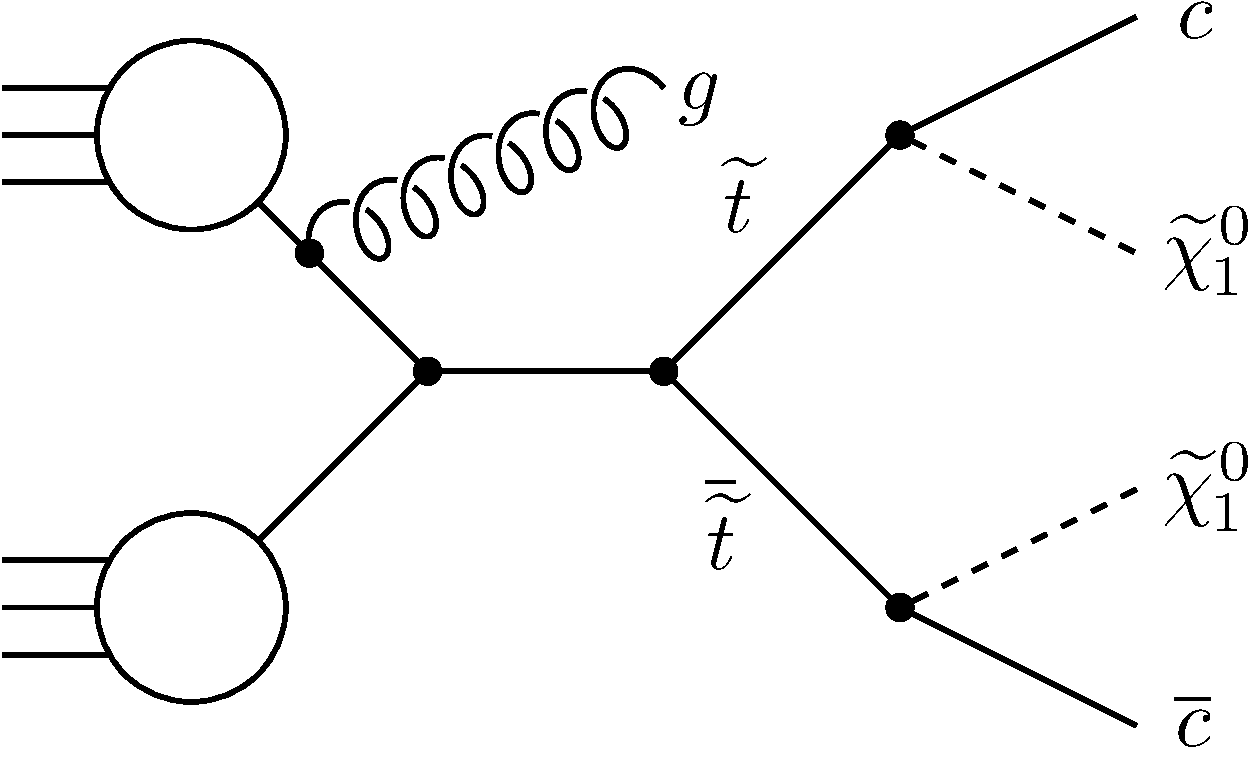
\includegraphics[scale=0.4]{Figures/sus13009/t2cc.pdf}
 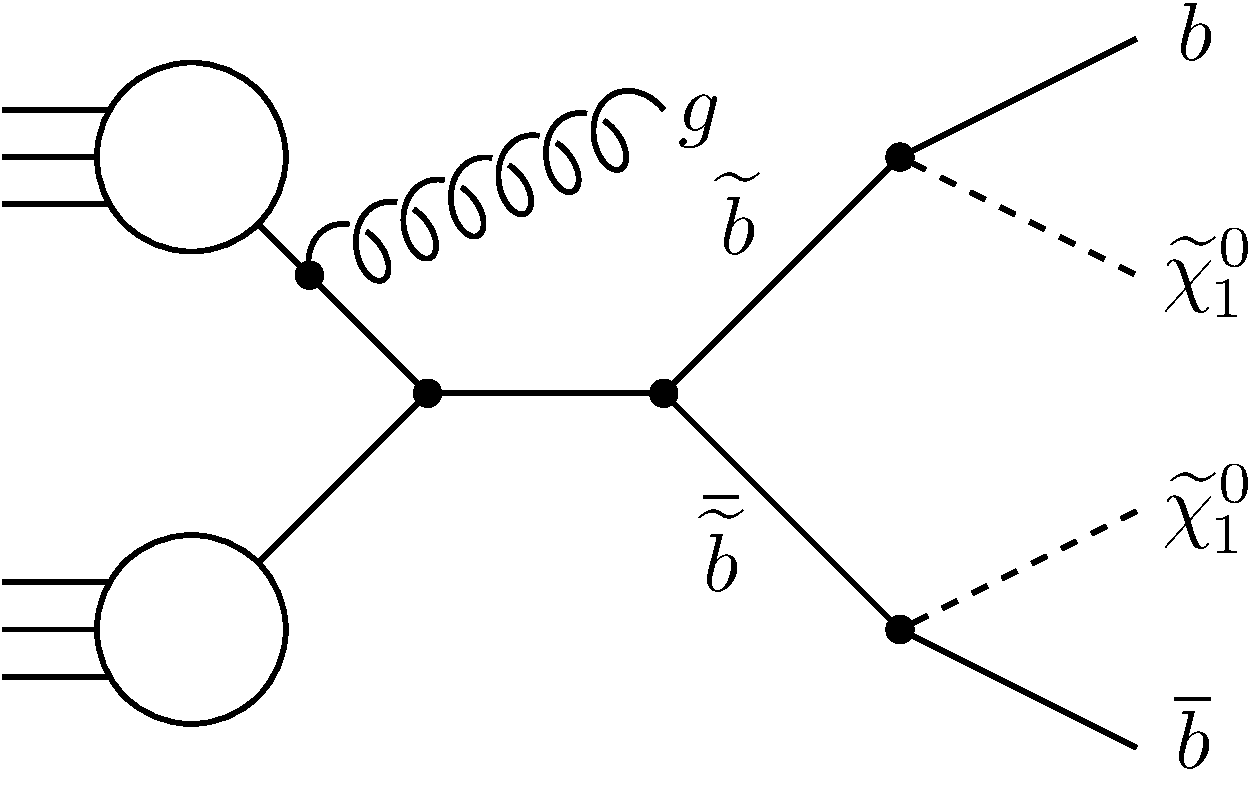
\includegraphics[scale=0.4]{Figures/sus13009/t2bb.pdf}
  \caption{Feynman diagrams of the signals probed. The top diagram shows the \ac{FCNC} process \ttwocc and the bottom diagram shows the process \ttwobb. In both cases, an \ac{ISR} gluon leads to an energetic jet, and balances the \MET due to \ac{LSP}s escaping the detector leaving no trace.}
	         \label{fig:feynmandiagrams}
  \end{center}
\end{figure}




\section{Data samples}
\label{sec:data}

The data for this search were collected using a combination of two triggers at the \ac{HLT}. 
The first requires events to have $\MET>120$~\GeV.
The second, a dedicated monojet trigger, requires a central jet ($|\eta|<2.6$) with $\pt>80~\GeV$ and \MET 
(calculated without muons) to be greater than 95 or 105~\GeV. 
These triggers also have coarse noise cleaning filters applied. 
The first has various requirements on the energy deposits in the \ac{HCAL} to cut out noisy events, 
and the second demands that the neutral energy deposited in the \ac{ECAL} is less than 95\% of the total energy deposited.
They are seeded by \ac{L1} triggers which require the missing transverse momentum, calculated using the coarse inputs available at \ac{L1}, to be greater than 36, 40 or 50~\GeV{} for the first trigger, or greater than 40~\GeV{} for the second trigger. 


Very few events with \MET{} below 100 GeV, where it is calculated offline using optimal object reconstruction,  will pass the analysis triggers described above that require \MET calculated online to be above 120~\GeV, or to be above 95 or 105~\GeV{} without muons. 
However, most events with \MET (reconstructed offline) above 200~\GeV{} will pass the same analysis triggers. 
It is therefore necessary to calculate the efficiency of these triggers in terms of the key analysis variables, \MET and the \pt of the leading jet, in order to find where best to place offline analysis cuts. 
An independent sample of events collected using a trigger requiring a single isolated muon with $\pt > 24$ and $|\eta|<2.4$ is used.
The efficiency is given by the ratio of the number events passing the analysis triggers to the number of events passing the reference trigger. 
Efficiencies are shown in the trigger turn-on curves in Figure~\ref{fig:trigger-1D} as a function of \MET\ and the \pt\ of the leading jet, as reconstructed offline. 
Here, the different colours show the different runs (A--D) of the \ac{LHC} during Run I.
The dedicated monojet trigger described above was introduced for Run C, which increased the efficiency of the combination of the triggers for lower values of \MET and leading jet \pt as compared to Runs A and B. 
%A two-dimensional plot of the trigger efficiency is shown as a function of the \MET\ and leading jet \pt\ in Figure~\ref{fig:trigger-2D}. 
The plots in Figure~\ref{fig:trigger-1D} show that the trigger paths become almost 100\% efficient at $\pt(j_{1})\sim110~\GeV$ and $\MET\sim220~\GeV$.

\begin{figure}%[!Hhtb]
  \begin{center}
 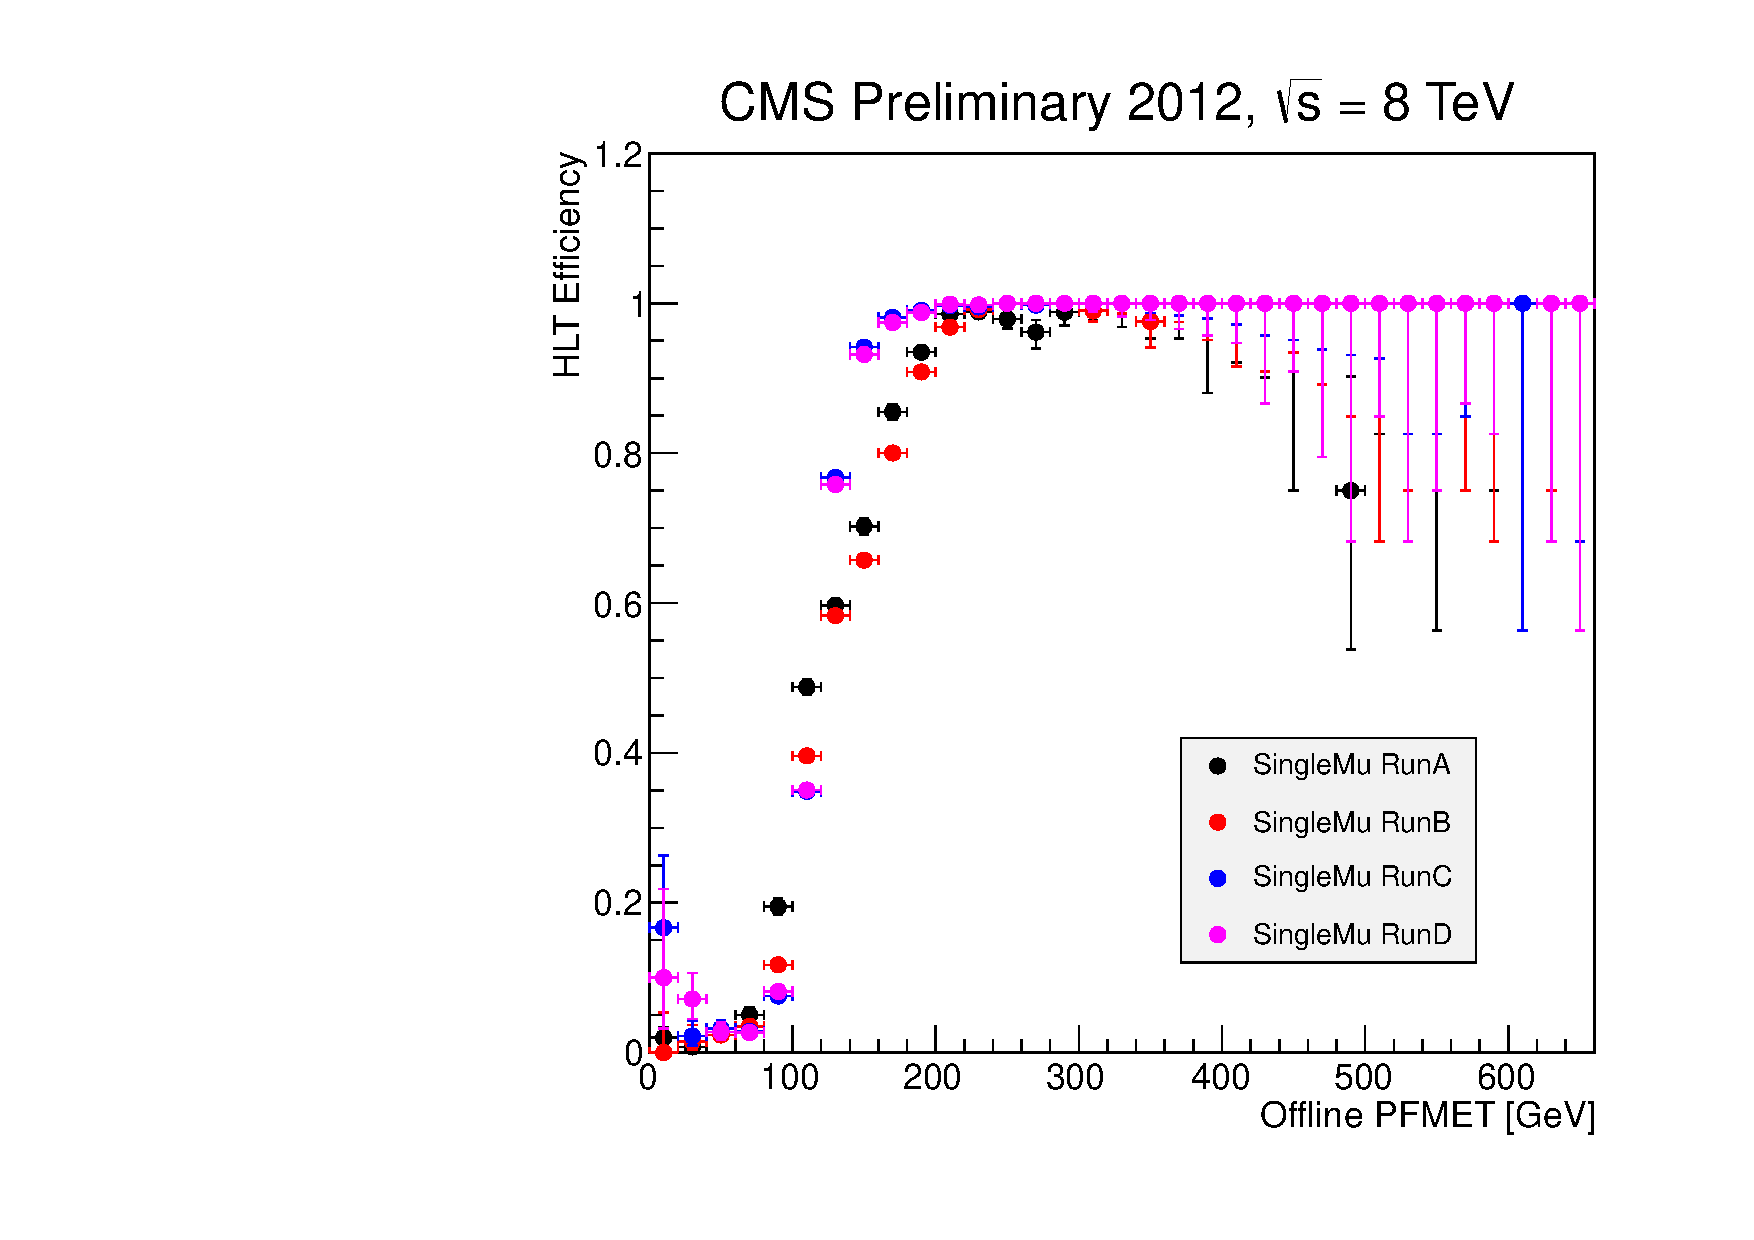
\includegraphics[scale=0.35]{Figures/sus13009/MET_OR.pdf}
 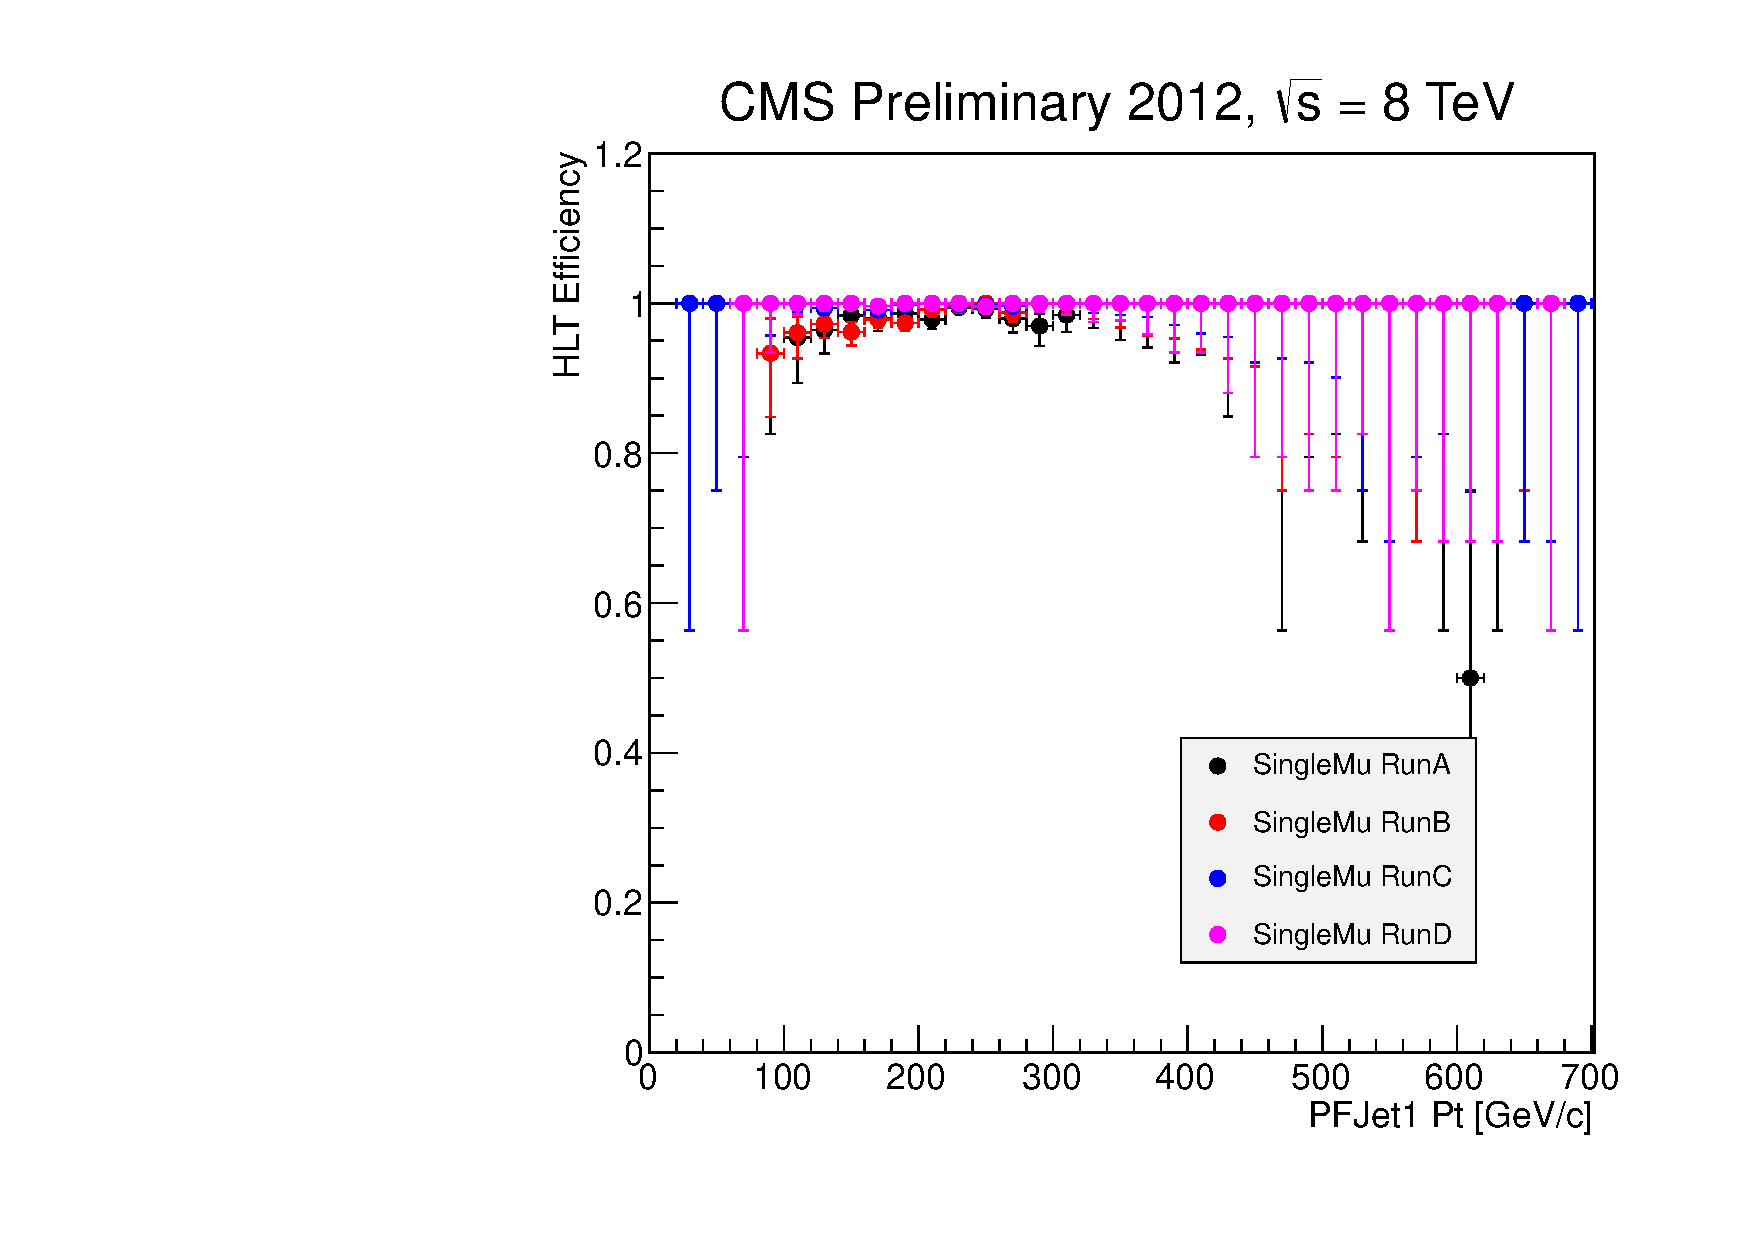
\includegraphics[scale=0.35]{Figures/sus13009/Jet1_OR.pdf}
  \caption{The trigger efficiency as a function of the \MET (left) and \pt of the leading jet (right).}
	         \label{fig:trigger-1D}
  \end{center}
\end{figure}

The specific datasets used for this analysis, along with their integrated luminosities, can be found in Table~\ref{tab:dataSets}. 
The data are from a `good-run' list of \ac{LHC} runs, in which each of the subsystems of the \ac{CMS} detector were operating well, and therefore event reconstruction was optimal.
Events were re-reconstructed using the \verb|CMSSW_5_3_9_patch3| release of the \ac{CMS} software (CMSSW), and form a part of the legacy dataset from Run I of \ac{CMS} running. 


\begin{table} %table 2    
    \begin{center}
    \caption{Datasets used in the search, which combine to give a total integrated luminosity of 19.7~\fbinv.}
     \begin{tabular}{clc}\hline
Era    &       Dataset  &  Int. Lumi. [$\pbinv$]\\ \hline
2012A & /MET/Run2012A-22Jan2013-v1/AOD & 889 \\
2012B & /MET/Run2012B-22Jan2013-v1/AOD & 4429 \\
2012C & /MET/Run2012C-22Jan2013-v1/AOD & 7152 \\
2012D & /METParked/Run2012D-22Jan2013-v1/AOD & 7315 \\ \hline
                \end{tabular}
                    \label{tab:dataSets}
\end{center}
\end{table}
%The data are reconstructed with the \verb+CMSSW_5_3_2_patch4+ release. %The good-run list and luminosity have been obtained by using the JSON files listed in~\cite{bib:ANA_data_JSON}, with all subsystems marked ``GOOD''.




%
\section{Background MC simulation} 
\label{sec:GEN}
\ac{MC} simulation of \ac{SM} backgrounds are used, directly and indirectly, to estimate the contribution of \ac{SM} backgrounds to the number of events in the search regions. 
The \ac{SM} processes considered are;  \W or \Z bosons produced in association with jets, top quark pair production (\ttbar), diboson ($\W\W{}$, $\W\Z{}$, $\Z\Z{}$, $\W\gamma{}$ and $\Z\gamma${}) production, single top quark events, and QCD multijet processes.

The simulation of each sample follows a similar procedure.
Events are generated using a matrix element event generator such as \MADGRAPH{}~\cite{madgraph,madgraph2}, which simulates the underlying process at parton level. 
The event is then passed through a parton showering programme, usually \PYTHIA{}~\cite{pythia,pythia8,pythia-z2} in which partons undergo hadronization: quarks hadronize into jets.
It is finally passed through a simulation of the CMS detector in order to mimic the detector's response to the event.
All simulated \ac{SM} background events have gone through a \GEANTfour~\cite{Geant4-1,Geant4-2} simulation of the detector. 
This is a `full' simulation, computationally expensive and providing accurate responses to the simulated physics objects.  
For simulation of signal (detailed later), a `fast' simulation~\cite{FASTSIM} is used instead as it is around 100 times faster to process each event and has a comparable accuracy.

Samples of \Z bosons decaying invisibly (\znunubr{}\,+\,jets), \ttbar, and diboson events 
are simulated using \MADGRAPH{}5 interfaced with \PYTHIA{}6.4.24. 
To evaluate the content of the proton in the initial state, the CTEQ6L \ac{PDFs} are used~\cite{CTEQ6}. 
%Samples are simulated using the custom CMS event tune Z2$^{*}$, which is derived from the Z1 tune~\cite{pythia-z2} which uses the CTEQ5L \ac{PDFs}, whereas the Z2$^{*}$ uses the CTEQ6L set.
Simulated Drell--Yan (\zellellbr{}\,+\,jets) and \wpj{} events are generated in the same way, where a cut has been placed on the transverse momentum of the boson, $\pt > 100$~\GeV, in order to increase the number of generated events that pass offline selection requirements (and where the production cross section has been modified accordingly).
QCD multijet events are generated with \PYTHIA{}6.4.24, using the CTEQ~6L1~\ac{PDFs}. 
Single top quark processes (s-channel, t-channel and tW-channel production) are generated using \POWHEG~\cite{powheg_st,powheg_tw}.
Decays of the $\tau$ lepton are simulated using the \TAUOLA{} 27.121.5 package~\cite{TAUOLA}. 

To ensure no double counting in phase space between the underlying event and the fragmentation and hadronization process, the MLM shower matching prescription~\cite{bib:GEN_MLM} is used, in which partons from the matrix element calculation are matched to jets resulting from the hadron shower.
In order to avoid double counting photons from the \PYTHIA shower in \wpj{} and $\W\gamma${} samples (and similarly for \zellellbr{}\,+\,jets and $\Z\gamma${} samples), 
events from the \wpj{} and \zellellbr{}\,+\,jets simulation which have a photon from \ac{ISR} or \ac{FSR}, of $\pt(\gamma)>5$~\GeV, are removed.


\section{Object reconstruction}
\label{sec:objectReco}

In Chapter~\ref{chap:detector} the CMS detector and reconstruction methods are discussed at length, including those used in this analysis. 
Here, the important features of the object reconstruction are recapped with additional details on the object definitions.

\subsection{Jets and \MET}

Jets and \MET are reconstructed using a \ac{PF}
technique~\cite{PFT-09-001}. The algorithm produces a unique list 
of particles in each event, using the combined information from all 
CMS subdetectors. This list is then used as input to the jet 
clustering, which reconstructs jets using the anti-k$_{\mathrm{t}}$
algorithm~\cite{bib:akjets} with a distance parameter of 0.5.  
The missing transverse energy vector \METv is computed as the negative vector 
sum of the transverse momenta of all particles reconstructed in the 
event.
Its magnitude is referred to as \MET.
Used throughout is the modification of this variable to exclude muons: the vector \METvmu is computed without muons, and its magnitude is referred to as \METmu. 

Jet energies are corrected to establish a uniform calorimeter 
response in $\eta$ and an absolute response in \pt, calibrated at 
the particle level.  
\ac{JES} corrections are derived from simulation, and a residual correction calculated by measuring the \pt balance in dijet and $\gamma$+jets events is applied to events in data~\cite{JETJINST} to account for differences in the \ac{JES} between data and simulation.
%The jet energy corrections used are `L2L3Residual' and `L1FastJet'.
To resolve any ambiguity in the reconstruction of jets and leptons, a jet is removed from the event if the energy fraction of an electron or muon in the jet is greater than 0.5.



\subsection{Leptons}
\label{sec:objectReco:lep}

Leptons are also reconstructed using the \ac{PF} algorithm and the definitions of objects are in accordance with the \ac{CMS} recommendations.
In addition to muons, electrons and $\tau$ leptons are also used in the analysis.
Muons either pass a ``loose'' or ``tight'' selection criteria (which has more stringent requirements). 
Electrons must pass a ``loose'' selection criteria, and the \ac{HPS} algorithm with ``loose'' criteria is used to reconstruct hadronically decaying $\tau$ leptons ($\tauh$).

A loose muon must have \pt{} greater than 10~\GeV{}, and be tagged as a Global or Tracker muon --- meaning that it must
have independent tracks from both the tracker and the muon systems that join together, or that a series of hits in the tracker matches up with at least one hit in the muon system~\cite{CMS-PAPER-MUO-10-004}. 
%
A tight muon must have \pt\,greater than $20~\GeV$ and be central --- $|\eta|<2.4$. 
It must also be considered a Global muon, with additional requirements on the global muon track. 
There must be at least one hit from the muon chambers included in the global track, and the $\chi^{2}$ of the global track must be less than 10. These requirements suppress mistaken muon identification as a result of hadronic punch-through from the \ac{HCAL} and the magnet, and suppress muons originating from in-flight decays.
There must also be hits in at least two of the muon stations, which acts to reduce the number of accidental track-to-segment matches.
In order to suppress the number of cosmic-ray muons (and further suppress muons from in-flight decays), the transverse impact parameter of the track ($d_{xy}$) as reconstructed in the tracker must be less than 2~mm from the primary vertex. 
Requiring the longitudinal impact parameter ($d_{z}$) to be less than 5~mm has a similar effect, as well as reducing the number of muons which originate from \ac{PU}.
Additional demands on the number of hits in the pixel system ($>0$) and the number of tracker layers with hits ($>5$) further suppress in-flight muon decays, and guarantee a good measurement of the muon \pt{}.

The electron identification used in the analysis is loose. To be classified as an electron, a track in the tracker must match to a supercluster in the \ac{ECAL}. 
The electron \pt must be greater than 10~\GeV{}, 
and the electron reconstruction avoids the gap between the \ac{ECAL} barrel and endcap where there is no instrumentation (and thus reconstruction is far from optimal): 
$1.44< |\eta| < 1.56 $. 
In addition, various simple parameters regarding the supercluster shower shape, matching between the \ac{ECAL} cluster and track, 
the ratio of energy deposited in the \ac{ECAL} and \ac{HCAL}, and impact parameters distinguish between primary electrons and those originating from bremsstrahlung and photon conversion. More information can be found in Ref.~\cite{CMS:elecReco}.

To ensure that electrons and muons are isolated --- not close to a jet or other object --- they must satisfy requirements on the isolation parameter $Iso$, defined as
\begin{equation}
Iso = \frac{\sum{\ET^{\text{charged hadrons}}}+ \sum{\ET^{\text{neutral hadrons}}}+ \sum{\ET^{\text{photons}}} }{\pt},
\end{equation} 
where the hadrons and photons are considered in a cone with radius $\Delta R=\sqrt{\Delta \phi ^{2} + \Delta \eta ^{2}}=0.4$ around the lepton direction.
Tight muons must have $Iso<0.12$, and loose muons must have $Iso<0.2$. 
Loose electrons must also have $Iso<0.2$.
Isolations are corrected for the effect of \ac{PU}. 
For charged particles, only those which are associated with the primary vertex in the event are considered, where this primary vertex is defined as that which has the largest sum of $\pt^{2}$ of all the tracks associated with it. 
The hadronization of \ac{PU} vertices leads to approximately twice 
the number of charged hadrons than neutral hadrons, 
so the energy within the isolation cone deposited by charged particles 
from \ac{PU} vertices is multiplied by 0.5 and subtracted from the neutral component~\cite{deltabeta_htautau7tev}.


The $\tau$ lepton decays hadronically 65\% of the time, with the dominant decay modes consisting of one or three charged $\pi^{\pm}$ mesons, and up to two neutral $\pi^{0}$ mesons.
The \ac{HPS} algorithm first reconstructs the $\pi^{0}$ component of the \tauh decay using a \ac{PF} anti-k$_{\rm t}$ seed jet with distance parameter 0.5, and then combines with charged hadrons to build a \tauh. 
`Strips' are constructed from \ac{PF} photons and electrons, starting with the most energetic electromagnetic particle within the seed jet, and combining all surrounding electromagnetic particles.
Strips with $\pt > 1$~\GeV{} are then combined with charged hadrons to provide a \tauh candidate. 
Here, the candidate must have $\pt > 20$~\GeV{} and $|\eta| < 2.3$ and the loose requirements of the algorithm are used which correspond to approximately 1\% of jets to be misidentified as a $\tauh$.
Similar corrections to account for \ac{PU} are applied as described above for the isolation parameter. 
More information can be found in Ref.~\cite{bib:HPStaus}. 
%It must pass the loose combined isolation discriminant (LooseCombinedIsolationDeltaBetaCorr)
%\item pass DecayModeFinding
%\item passes AgainstElectronLoose discriminant
%\item passes AgainstMuonTight2 discriminant



\section{Event selection}
\label{sec:ANA}

The aim is to select signal candidate events while rejecting as much background as possible.
A final state with one, high \pt leading jet, and large \MET from the LSPs leaving the detector form the basis of the event selection in order to be sensitive to compressed \ac{SUSY} signatures.

\subsection{Event Cleaning}

The first stage of the event selection, after the trigger, is to reject any events that have passed the trigger due to instrumental noise or non-collision backgrounds.

Events are required to have at least one well-reconstructed primary vertex~\cite{bib:ANA_Tk}, where it is reconstructed in a 24~cm window along the beam axis, within a radius of $\rho<2$~cm orthogonal to the plane of the beam. %The number of degrees of freedom must be less than 4.
To reject events that have ``scraping'' tracks due to beam-gas interactions close to the interaction point, in events where there are 10 or more tracks at least 25\% must be good quality; that is, satisfy various requirements on the number of hits, the \pt of the track, the $\chi^{2}$ of the combination of hits which build the track etc.
To remove events with spurious \MET reconstruction, different methods of calculating the \MET are compared. The value of \MET, reconstructed using the \ac{PF} algorithm, must be comparable with the \MET calculated using calorimetric information only: events with (PF \MET - calo \MET)$ > 2 \times$ calo \MET are discarded.



%event cleaning
% The reported TOC/TEC problem \cite{bib:TOCTEC} has been shown to have a negligable effect here.
% There is a large discrepancy between PFMET and caloMET in affected events, 
% see Appendix~\ref{toctec} for comparison between PFMET and caloMET which shows no significant discrepancies between the two. 
% The requirement on PFMET and caloMET removes the majority of these events, and those remaining have been visually inspected.


Beam-halo and other beam-related backgrounds~\cite{bib:ANA_BeamHalo}, which arise when the beams interact with the beam pipes, 
can deposit energy in both the \ac{ECAL} and \ac{HCAL} leaving no associated tracks.
Cosmic muons also can give rise to fake \MET, 
or leave similarly spurious deposits - leading to fake jets - as they deposit energy in one or more of the subdetectors while leaving no tracks, or tracks which do not originate from the primary vertex.
Similarly, instrumental noise can lead to large apparent deposits in the \ac{ECAL} or \ac{HCAL}. 
Stringent requirements are therefore placed on the neutral and charged hadronic and electromagnetic content of jets:
\begin{itemize}
\item Leading jet charged electromagnetic fraction $<$ 0.7
\item Leading jet charged hadronic fraction $>$ 0.2
\item Leading jet neutral electromagnetic fraction $<$ 0.7
\item Leading jet neutral hadronic fraction $<$ 0.7
\item Second jet neutral electromagnetic fraction $<$ 0.9
\item Second jet neutral hadronic fraction $<$ 0.7
\end{itemize}
These conditions also reject high \pt{} photons and electrons which are misidentified as jets due to 
energy deposits in the \ac{HCAL}; the energies associated with neutral hadrons in the 
ECAL and HCAL must sum to less than 70\% of the total jet energy.
In addition, jets are also required to pass a loose identification criterion which rejects fake jets due to calorimeter noise. 

The distributions for the neutral and charged energy fractions of the first and second jet in events (where jets are \pt{} ordered) before and after these noise cleaning cuts are applied are shown in Figures~\ref{fig:ANA_energy_fraction_cleanup} and~\ref{fig:ANA_energy_fraction_cleanup_cut}. 
They are very effective at removing noisy events, with good data/MC agreement after the cuts have been applied.

%The application of all event cleaning criteria results in the loss of 4.2\% of the events for a representative ADD signal, 1.8\% of events for a representative dark matter model and 6.7\% for a representative Unparticle signal.

\begin{figure}[!Hhtb]%[tb]
  \begin{center}
  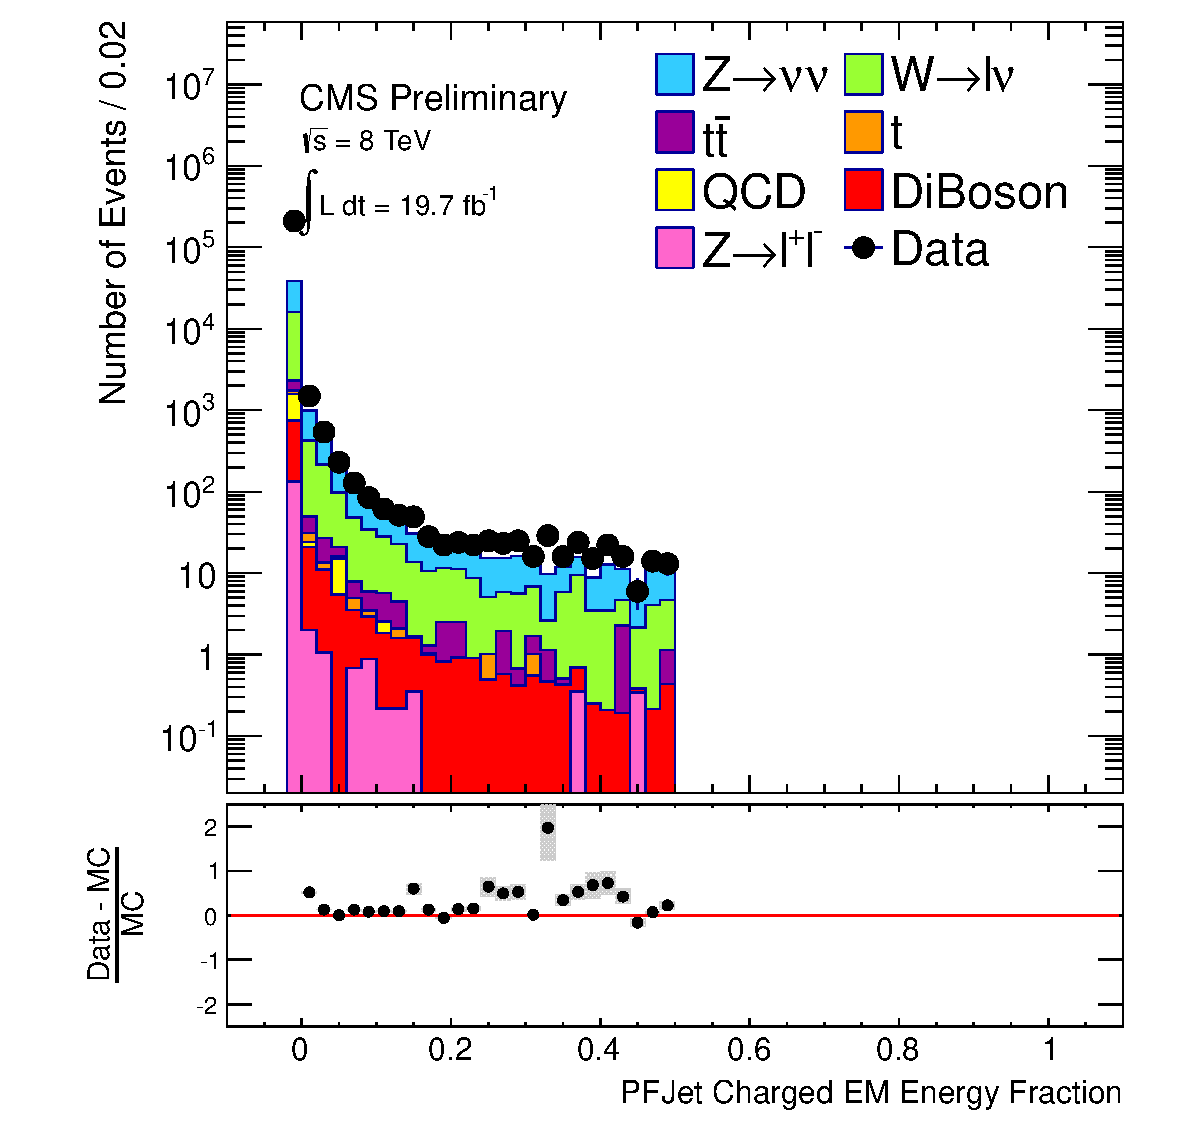
\includegraphics[scale=0.31]     {Figures/sus13009/nocut/prelimLabels/PFAK5JetChaEmEngFrac.pdf}
  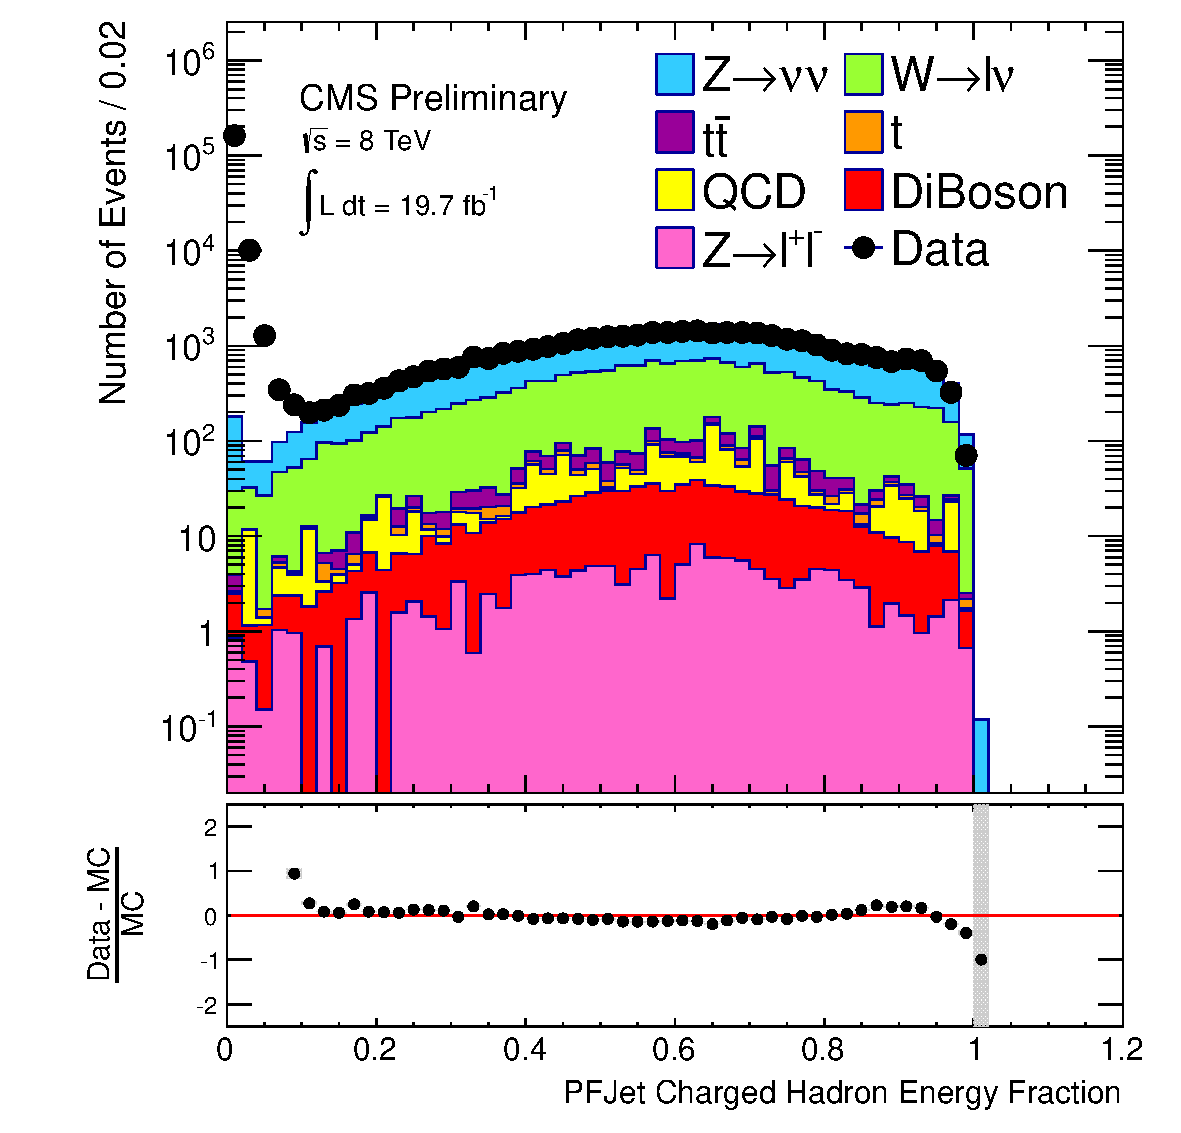
\includegraphics[scale=0.31]     {Figures/sus13009/nocut/prelimLabels/PFAK5JetChaHadEngFrac.pdf}
  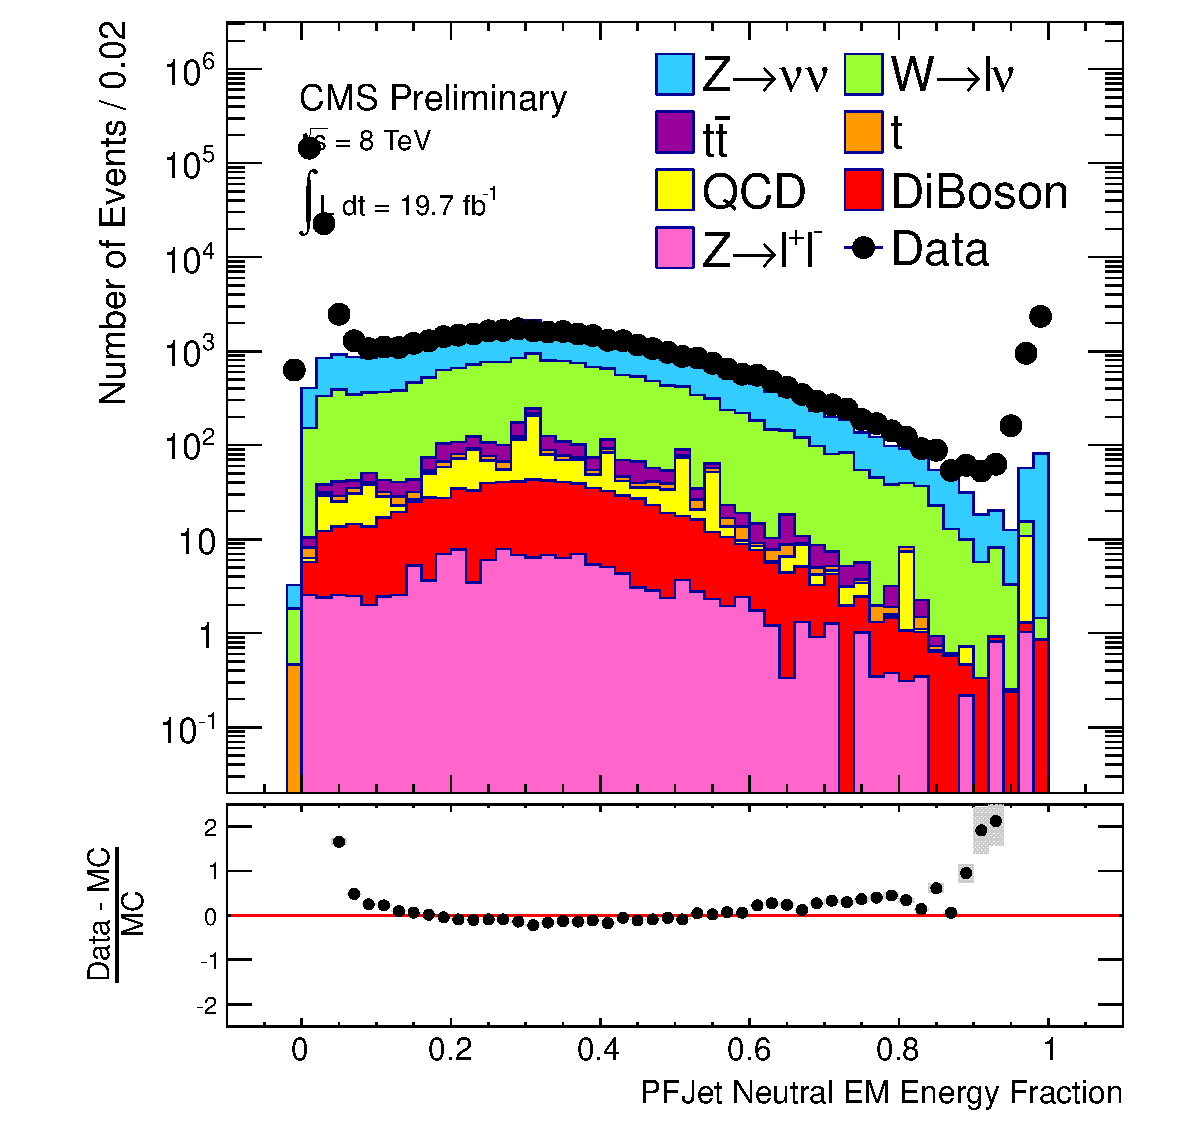
\includegraphics[scale=0.31]     {Figures/sus13009/nocut/prelimLabels/PFAK5JetNeuEmEngFrac.pdf}
  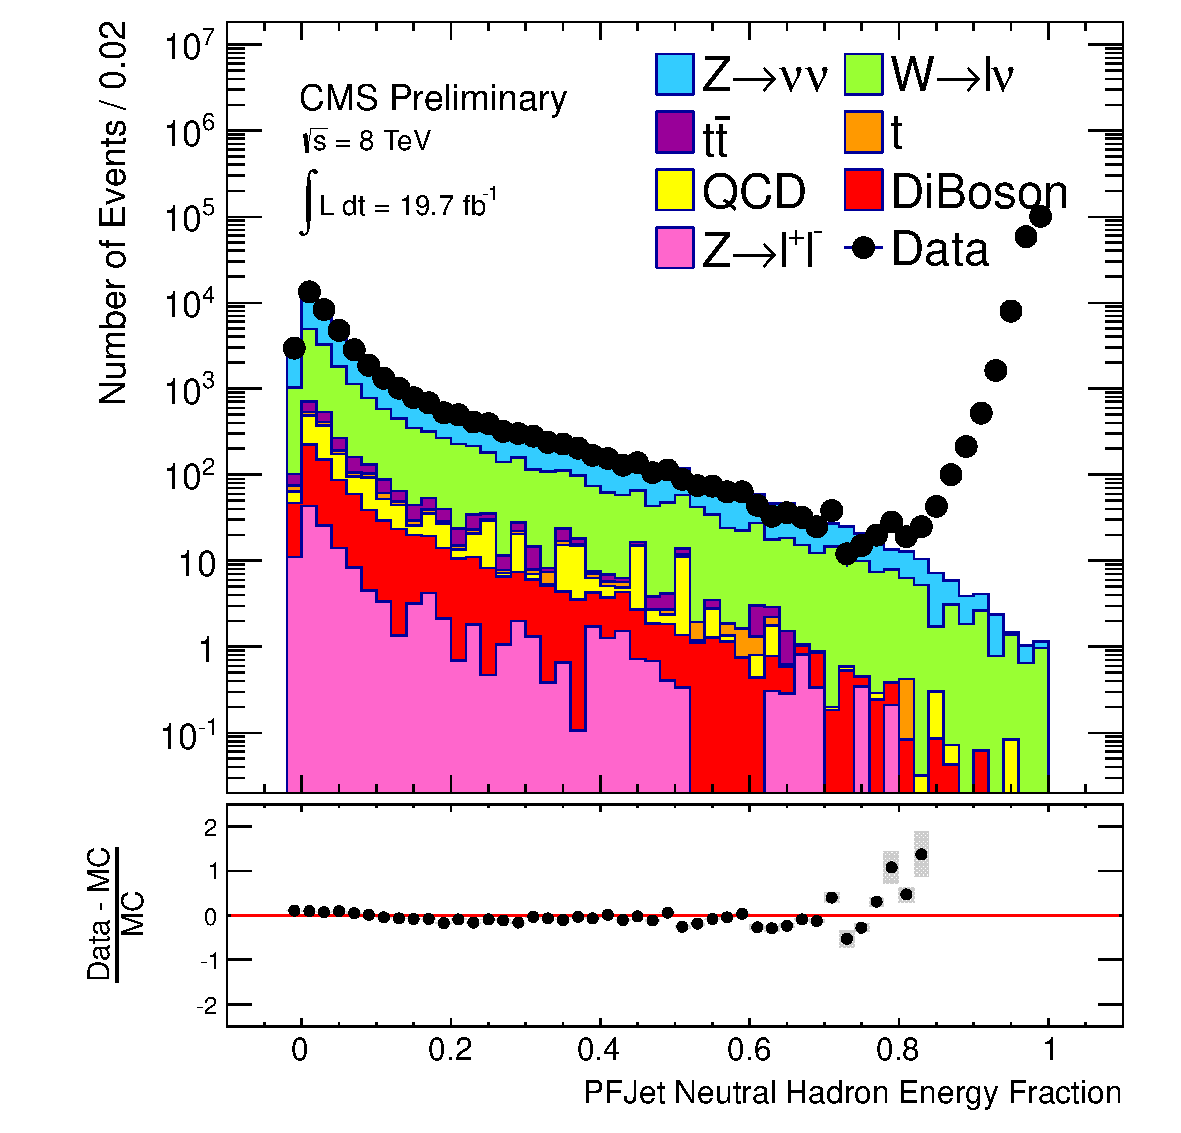
\includegraphics[scale=0.31]     {Figures/sus13009/nocut/prelimLabels/PFAK5JetNeuHadEngFrac.pdf}
  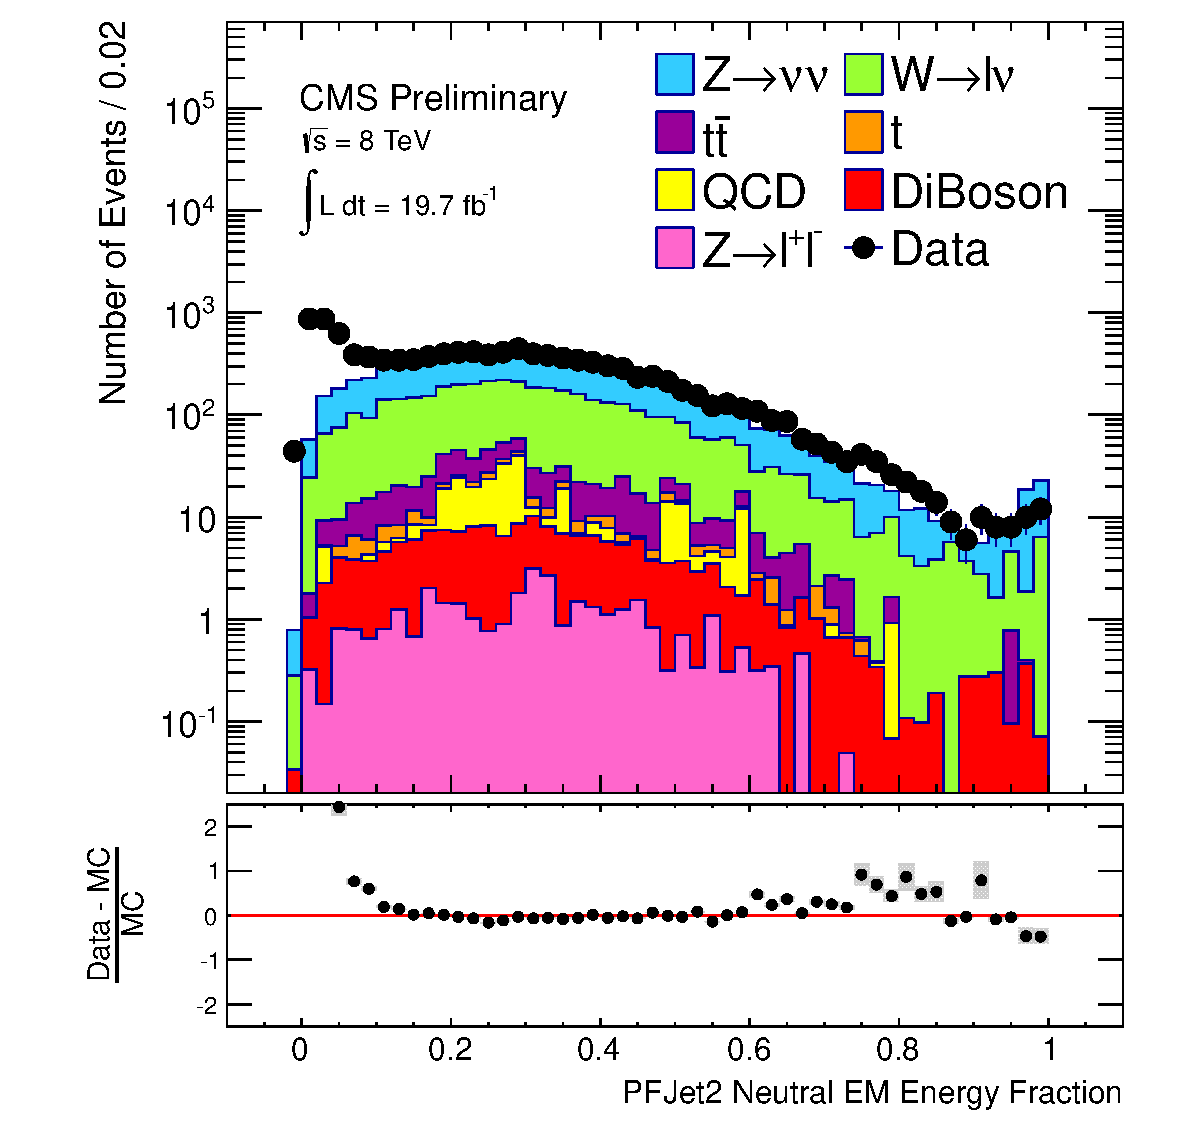
\includegraphics[scale=0.31]     {Figures/sus13009/nocut/prelimLabels/PFAK5JetNeuEmEngFrac2.pdf}
  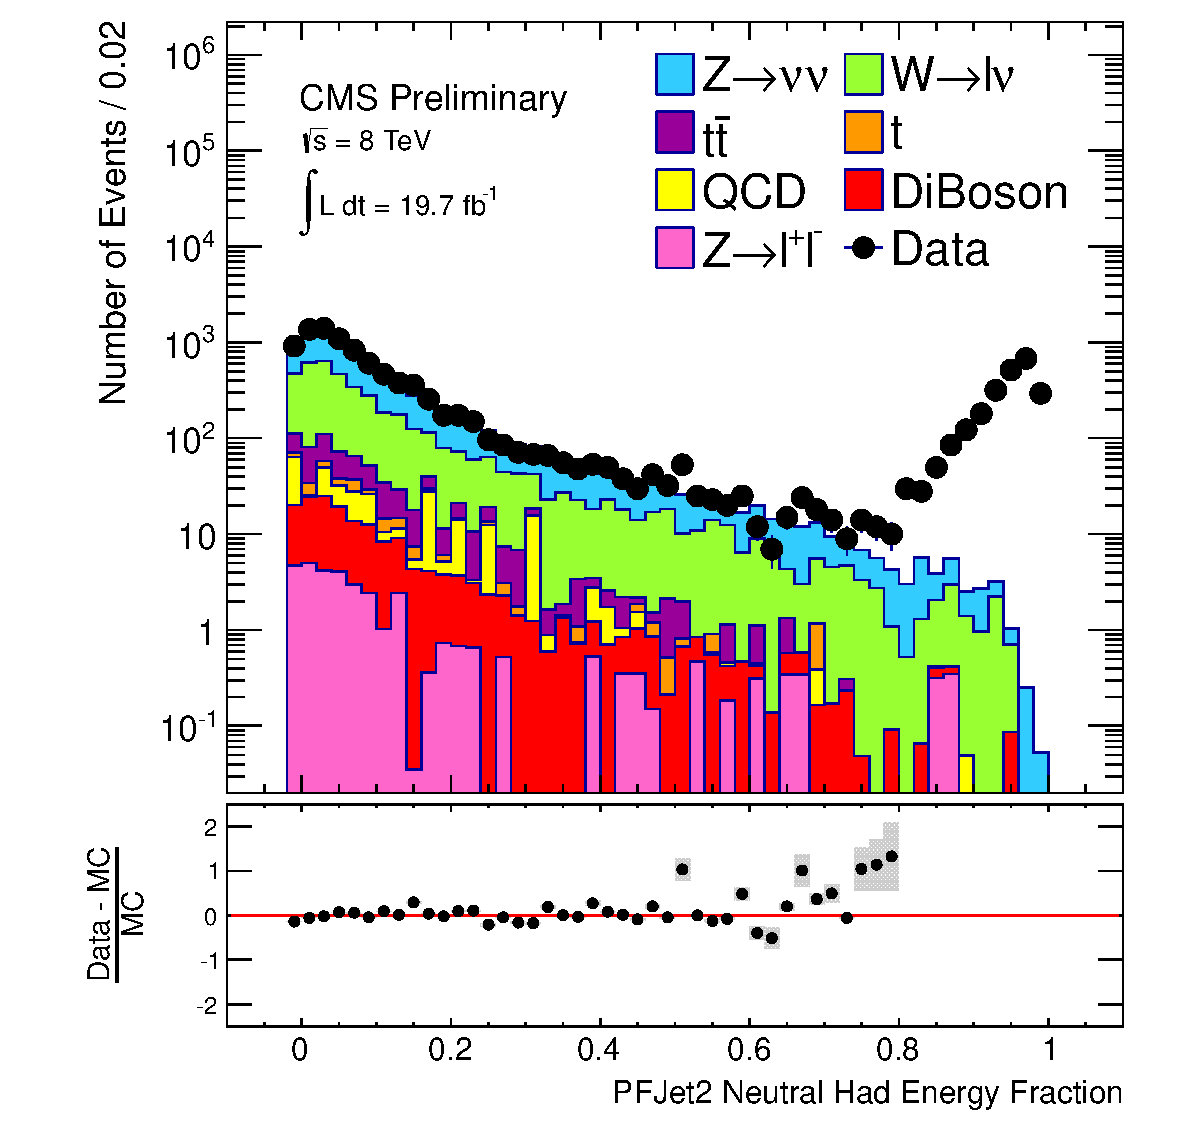
\includegraphics[scale=0.31]     {Figures/sus13009/nocut/prelimLabels/PFAK5JetNeuHadEngFrac2.pdf}
  \caption{Hadronic and electromagnetic energy fractions from charged 
and neutral particles, before clean-up cuts on these quantities are 
applied. We require the charged 
hadronic fraction of the jet to be above 20\% and the neutral electromagnetic and hadronic energy fractions to be below 70\% of the total leading jet energy.
We require the neutral electromagnetic energy to be below 90\% and the neutral hadronic energy of the second jet to be below 70\% of the total second leading jet energy. }
         \label{fig:ANA_energy_fraction_cleanup}
  \end{center}
\end{figure}
%
\begin{figure}[!Hhtb]
  \begin{center}
  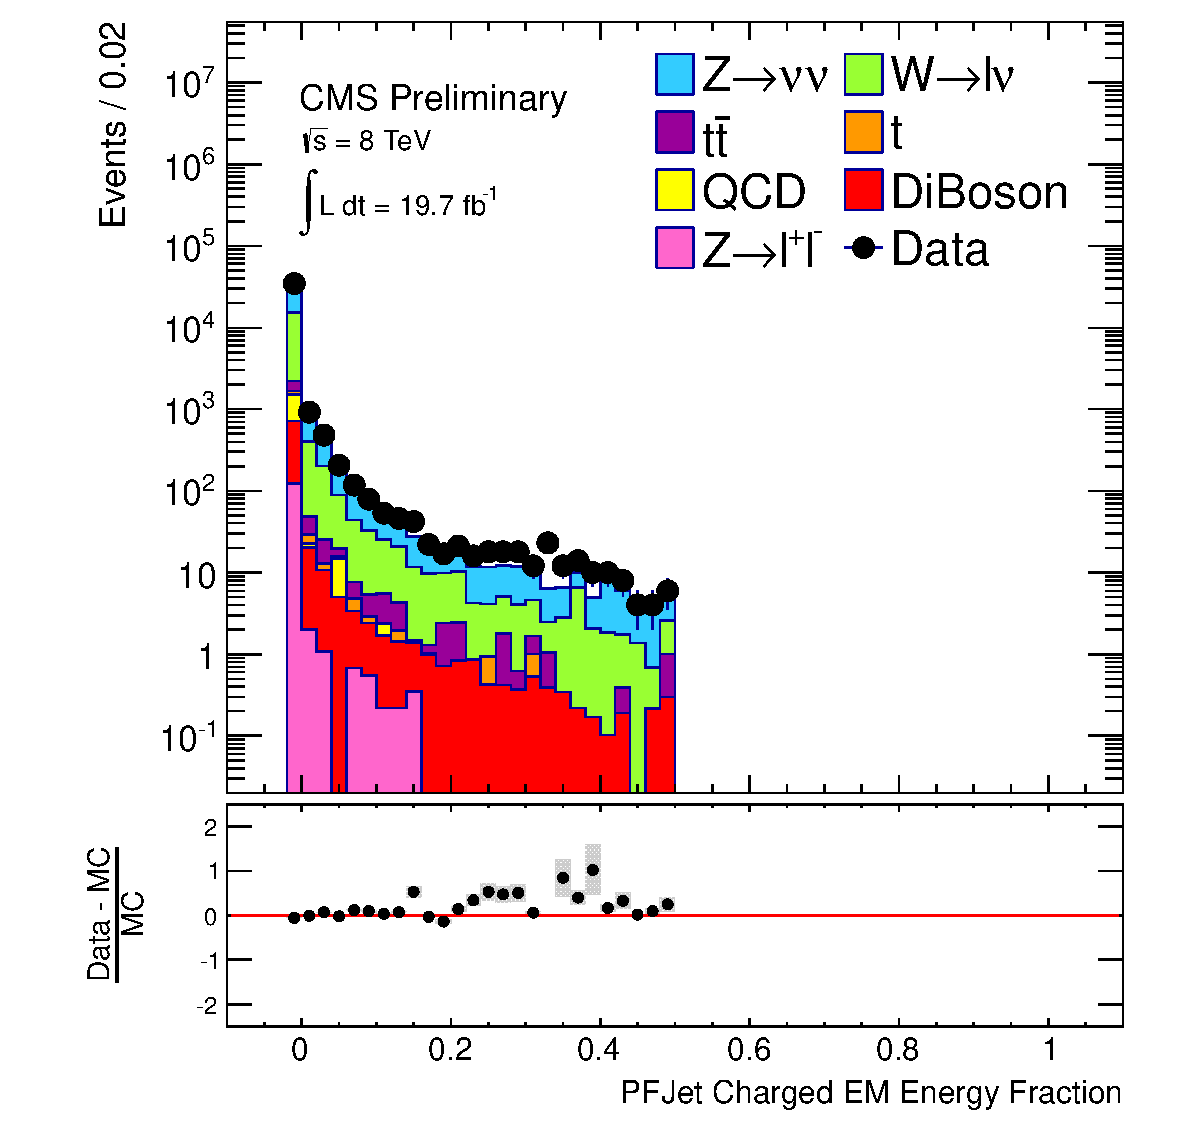
\includegraphics[scale=0.31]     {Figures/sus13009/nocut/prelimLabels/cut/PFAK5JetChaEmEngFrac.pdf}
  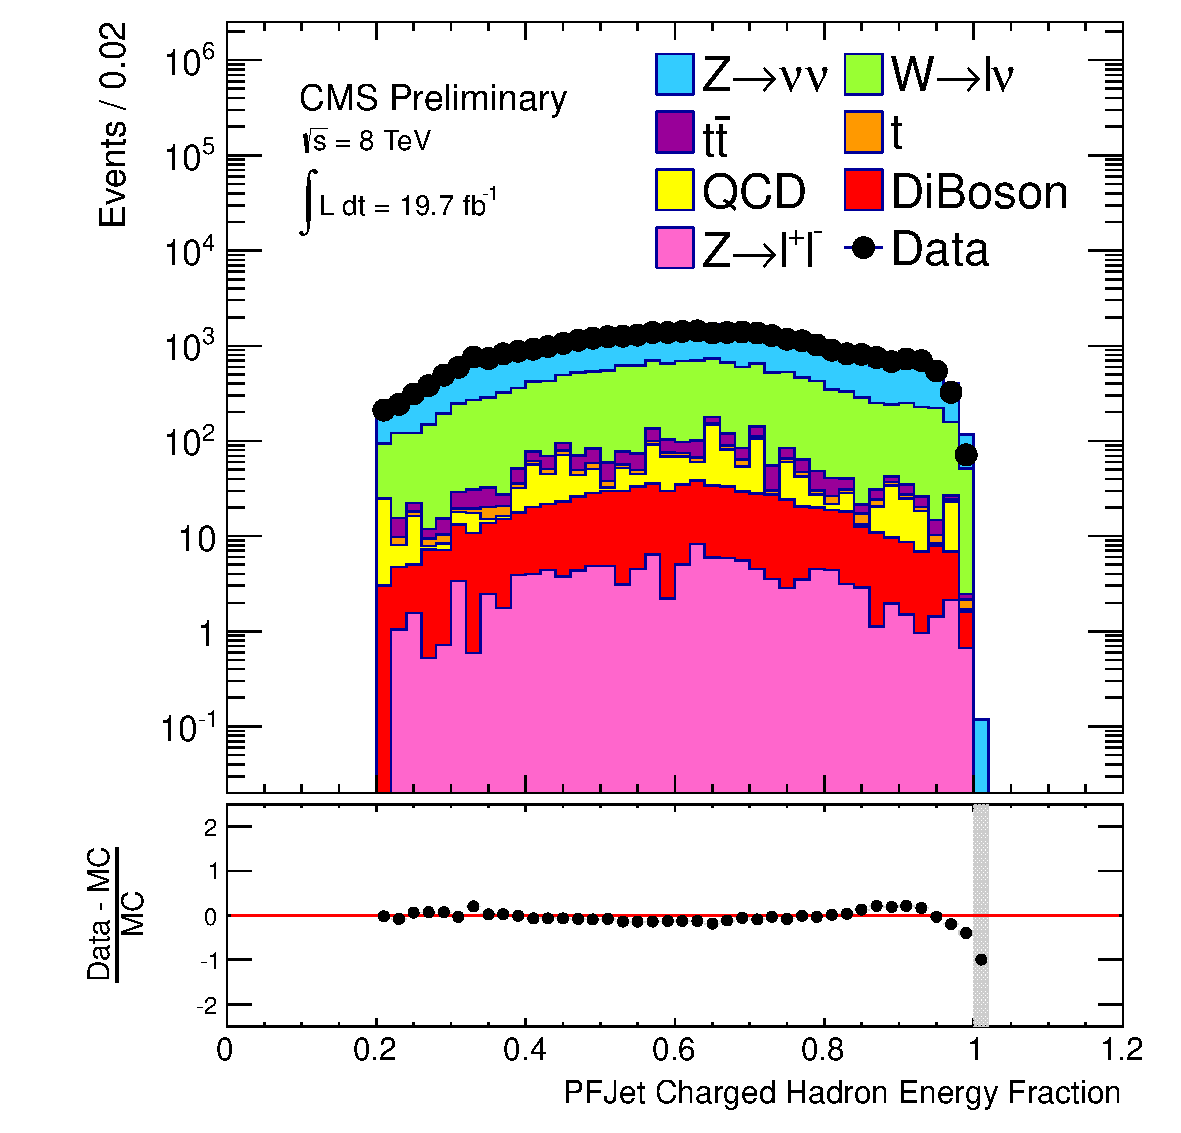
\includegraphics[scale=0.31]     {Figures/sus13009/nocut/prelimLabels/cut/PFAK5JetChaHadEngFrac.pdf}
  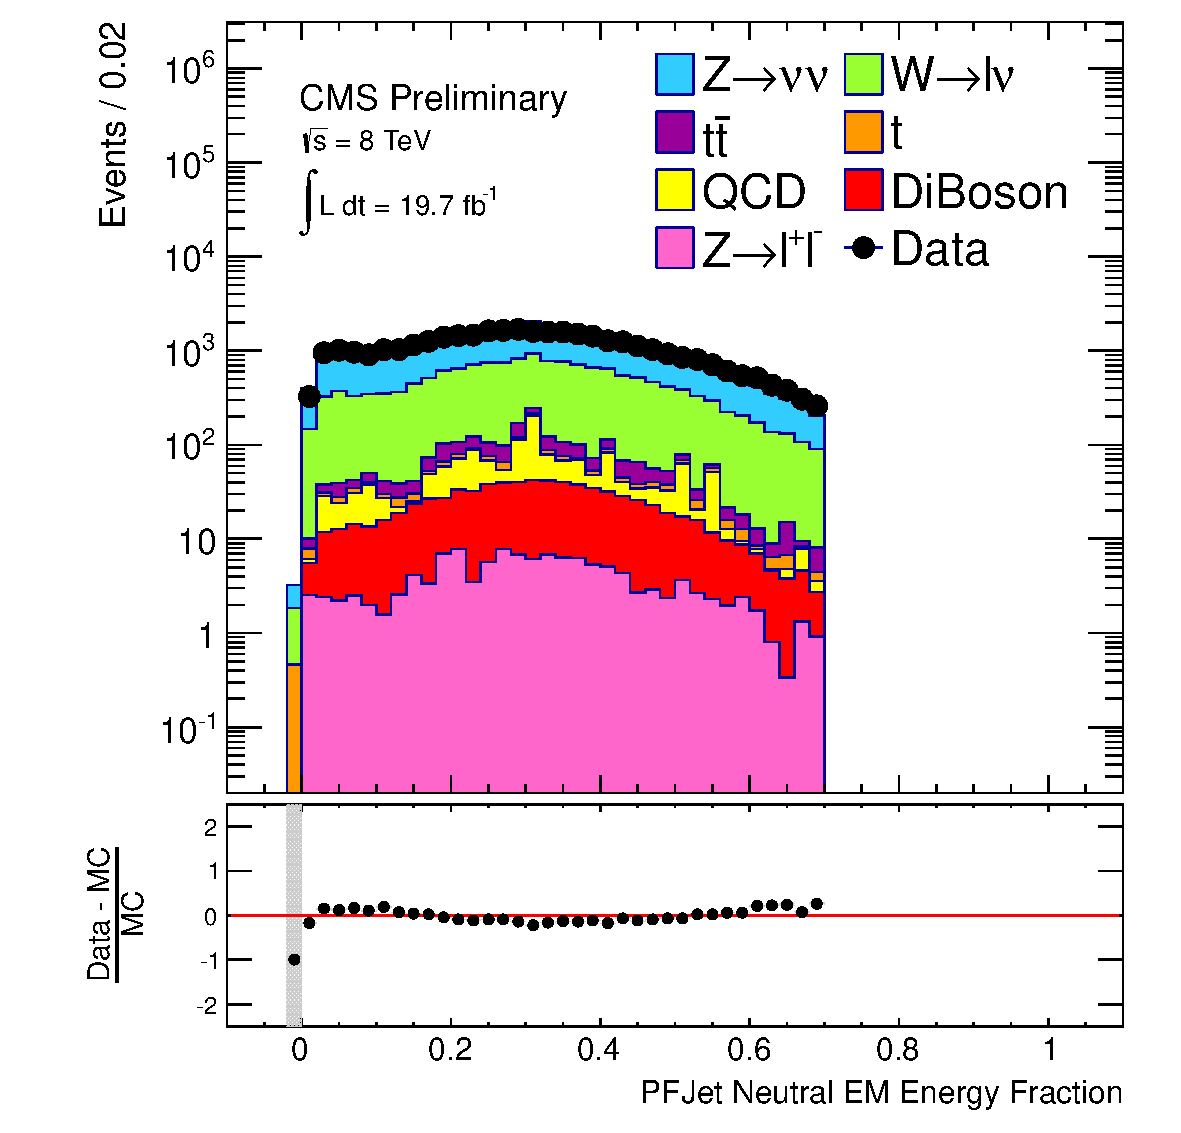
\includegraphics[scale=0.31]     {Figures/sus13009/nocut/prelimLabels/cut/PFAK5JetNeuEmEngFrac.pdf}
  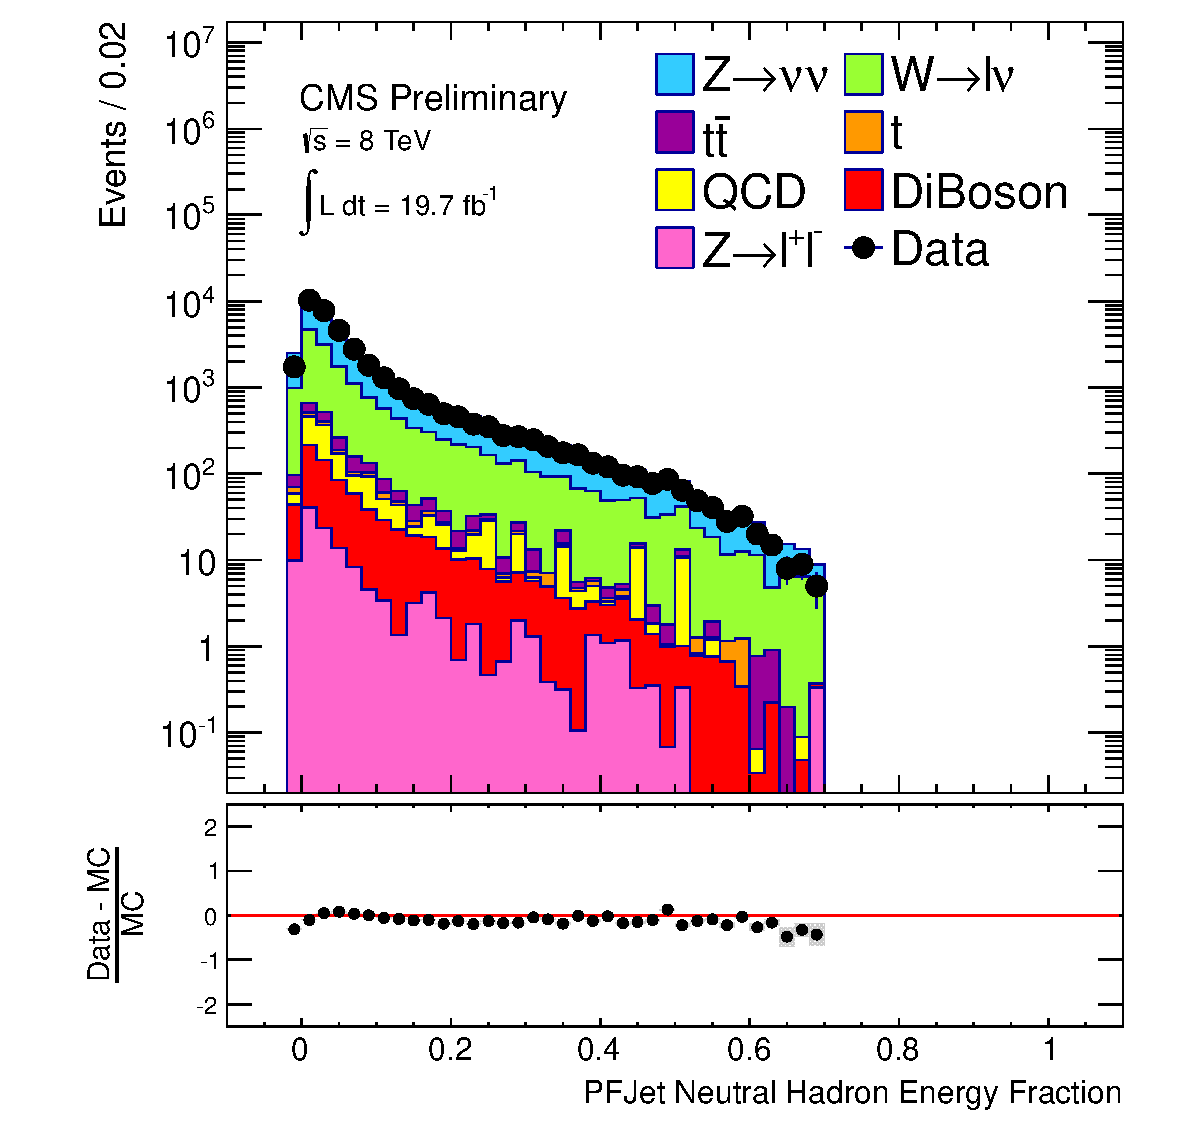
\includegraphics[scale=0.31]     {Figures/sus13009/nocut/prelimLabels/cut/PFAK5JetNeuHadEngFrac.pdf}
  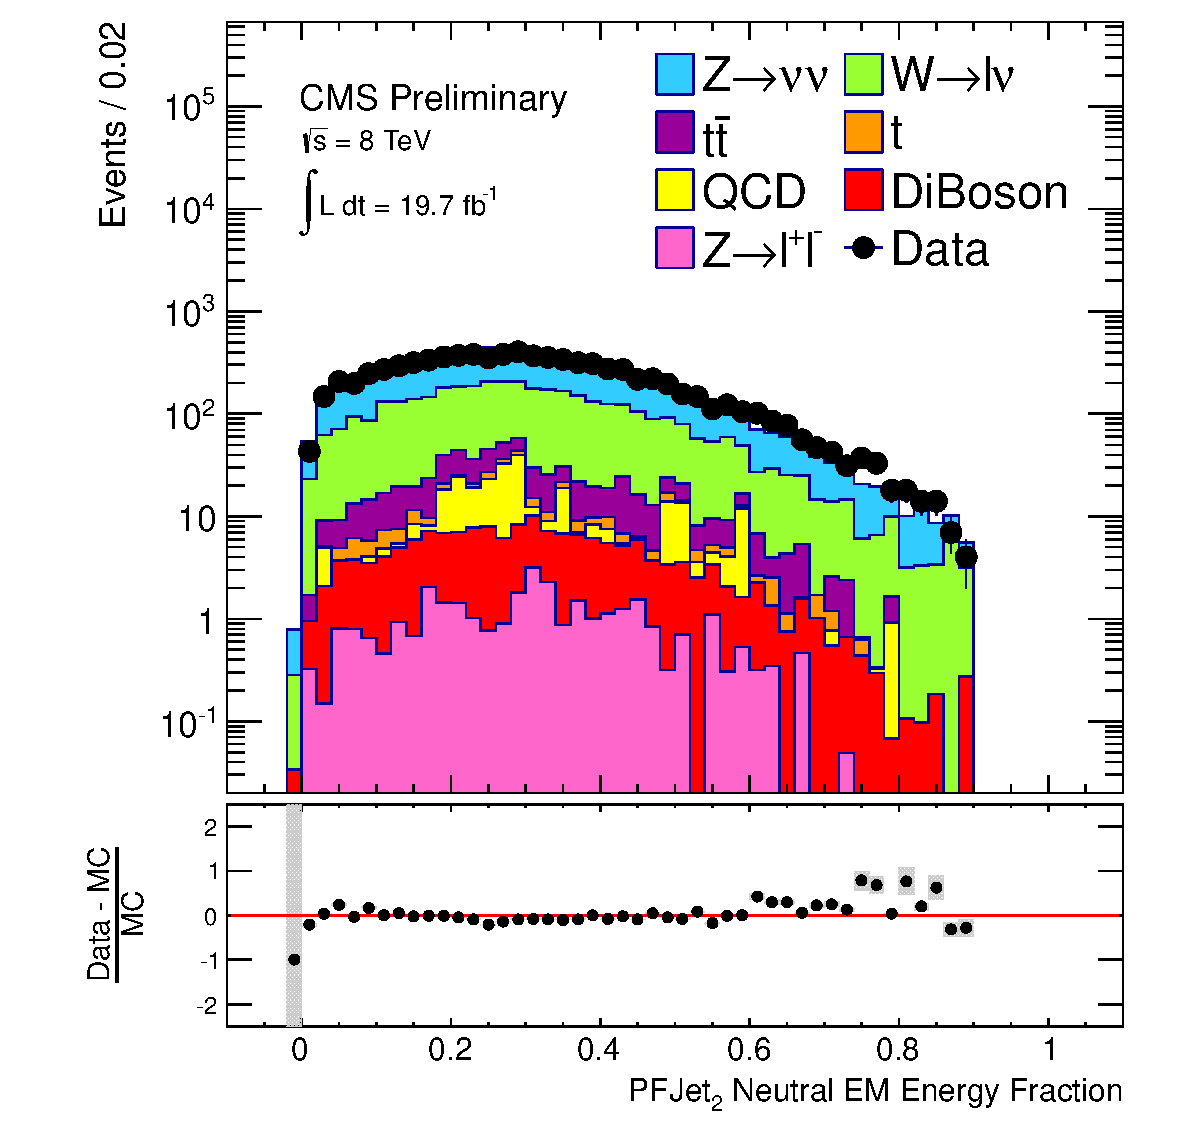
\includegraphics[scale=0.31]     {Figures/sus13009/nocut/prelimLabels/cut/PFAK5JetNeuEmEngFrac2.pdf}
  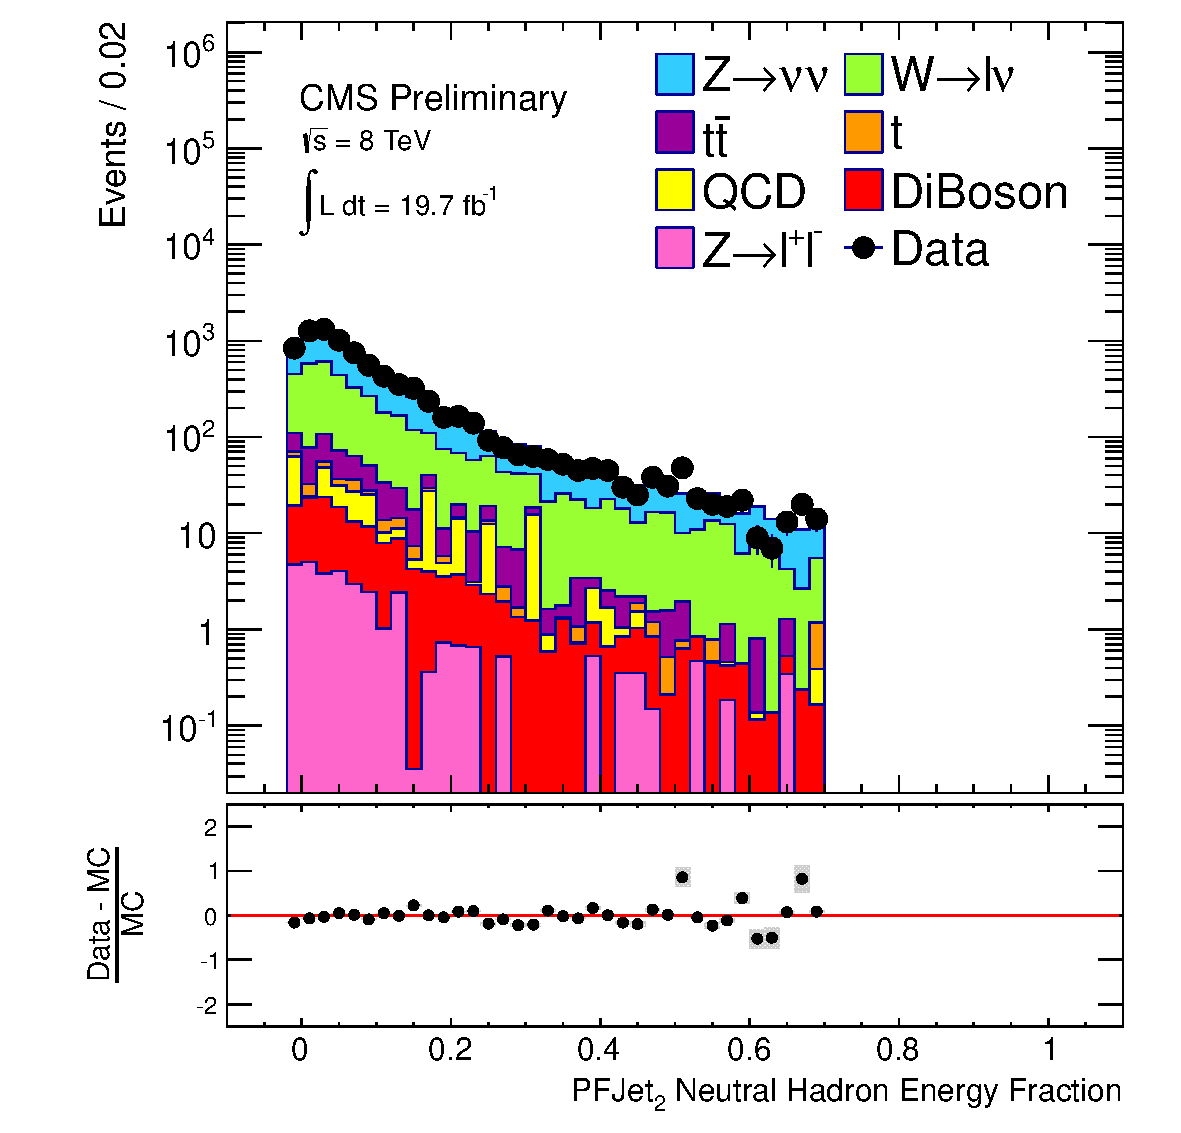
\includegraphics[scale=0.31]     {Figures/sus13009/nocut/prelimLabels/cut/PFAK5JetNeuHadEngFrac2.pdf}
  \caption{Hadronic and electromagnetic energy fractions from charged 
and neutral particles, after clean-up cuts on these quantities are 
applied.}
         \label{fig:ANA_energy_fraction_cleanup_cut}
  \end{center}
\end{figure}


\subsection{Search region event selection}

Once events passing the trigger have been filtered to remove noise and fakes, 
events are selected to optimize signal acceptance while rejecting as much background as possible.

To satisfy trigger requirements, and ensure most events comfortably pass the \ac{HLT} trigger selection, 
events are required to have $\METmu > 200$~\GeV{} and the most energetic jet ($\jet_1$) in the event is required 
to have $\pt(\jet_1)>110~\GeV$ and $|\eta(\jet{}_1)|<2.4$.
%§c
Signal acceptance is increased by allowing events where there is a second jet $(\jet_2)$ originating from \ac{ISR} (or \ac{FSR}); 
however the signal also has soft final-state jets originating from the sparticle decay products.
%
To ensure that these soft final-state jets coming from charm or bottom quarks remain invisible within the event selection,
%
and a monojet signature is maintained,
the \pt{} threshold at which the second and third jets are counted must be high enough that
the soft-hadronic (signal) decay products 
fall below it for a good range of signal phase space 
%(and therefore remain invisible in the event selection), 
while keeping the QCD multijet background at a manageable level.
%
Figure~\ref{stopj2pT} shows the \pt{} distribution of charm quarks, taken from simulation, 
for a few representative mass hypotheses in the process $\ttwocc$.
%
Placing the jet counting threshold at $\pt >60$~\GeV, and requiring $|\eta| < 4.5$,
is a good compromise between signal efficiency and background rejection.
%
Events are therefore vetoed if they contain more than two jets,
where $\pt(\jet_{1})>110$~\GeV{} and $|\eta|<2.4$; $\pt(\jet_{2})>60$~\GeV{} and $|\eta|<4.5$; 
and the third jet is counted (and the event rejected) if it has $\pt(\jet_{3})>60$~\GeV{} and $|\eta|<4.5$.
A monojet-like topology in signal events is therefore maintained, 
allowing the search to be sensitive to both highly compressed spectra
and extending the scope to larger mass differences.  

\begin{figure*}%[tb]
  \begin{center}
  \includegraphics[scale=0.45]{Figures/sus13009/charmpt.pdf}
  \caption{Charm quark \pt{} spectra for mass splittings across the phase space range, $m_{\sTop}-m_{\chiOneZero}=10, 30, 80~\GeV$, for a top squark mass of 150~\GeV. Taken from Ref.~\cite{sus14001}.
         \label{stopj2pT}}
  \end{center}
\end{figure*}

To reduce the \ac{QCD} dijet background, if two jets are present in the event, they must not be back-to-back: 
$\Delta \phi (\jet_1,\jet_2) < 2.5$. 
The multijet background is largely rejected by the \njets$\le2$ requirement.

Electroweak backgrounds in which a \W{} or \Z{}-boson is produced in association with a jet can lead to large \MET as leptonic decays can lead to neutrinos or to mismeasured energy.
In order to reduce the background from such \Z{} and \W-boson decays in the search regions, events
with leptons are rejected. 
Events containing one or more loose electrons with $\pt > 10$~\GeV{} (where loose requirements are detailed in Section~\ref{sec:objectReco}) are rejected. 
Similarly, events containing any loose muons with $\pt > 10$ \GeV{} are also rejected. 
In addition, events containing hadronically decaying $\tau$ leptons are vetoed, where $\tauh$ are reconstructed using the \ac{HPS} algorithm as described in Section~\ref{sec:objectReco}.
The vetoes here use loose requirements of object reconstruction, to reject as many leptons --- and as much of the electroweak background --- as possible.

A trigger efficiency of unity is ensured by requiring $\METmu>250~\GeV$. Search regions are then defined by thresholds of the leading jet $\pt$; $\pt(\jet_{1}) >$ 250, 300, 350, 400, 450, 500 and 550~\GeV.
These are inclusive search regions, determined by the hardness of the \ac{ISR} jet in each event.
Typically, for a larger \sTop{} mass, there is a larger boost to the $\sTop\santiTop${} system --- see Figure~\ref{stopstoppT}. 
By having many, inclusive, search regions, sensitivity to a range of $\sTop${} (and $\sBot${}) masses is gained.  
The baseline search region is defined by the above selection requirements and a leading jet threshold of 250~\GeV.

\begin{figure*}%[tb]
  \begin{center}
  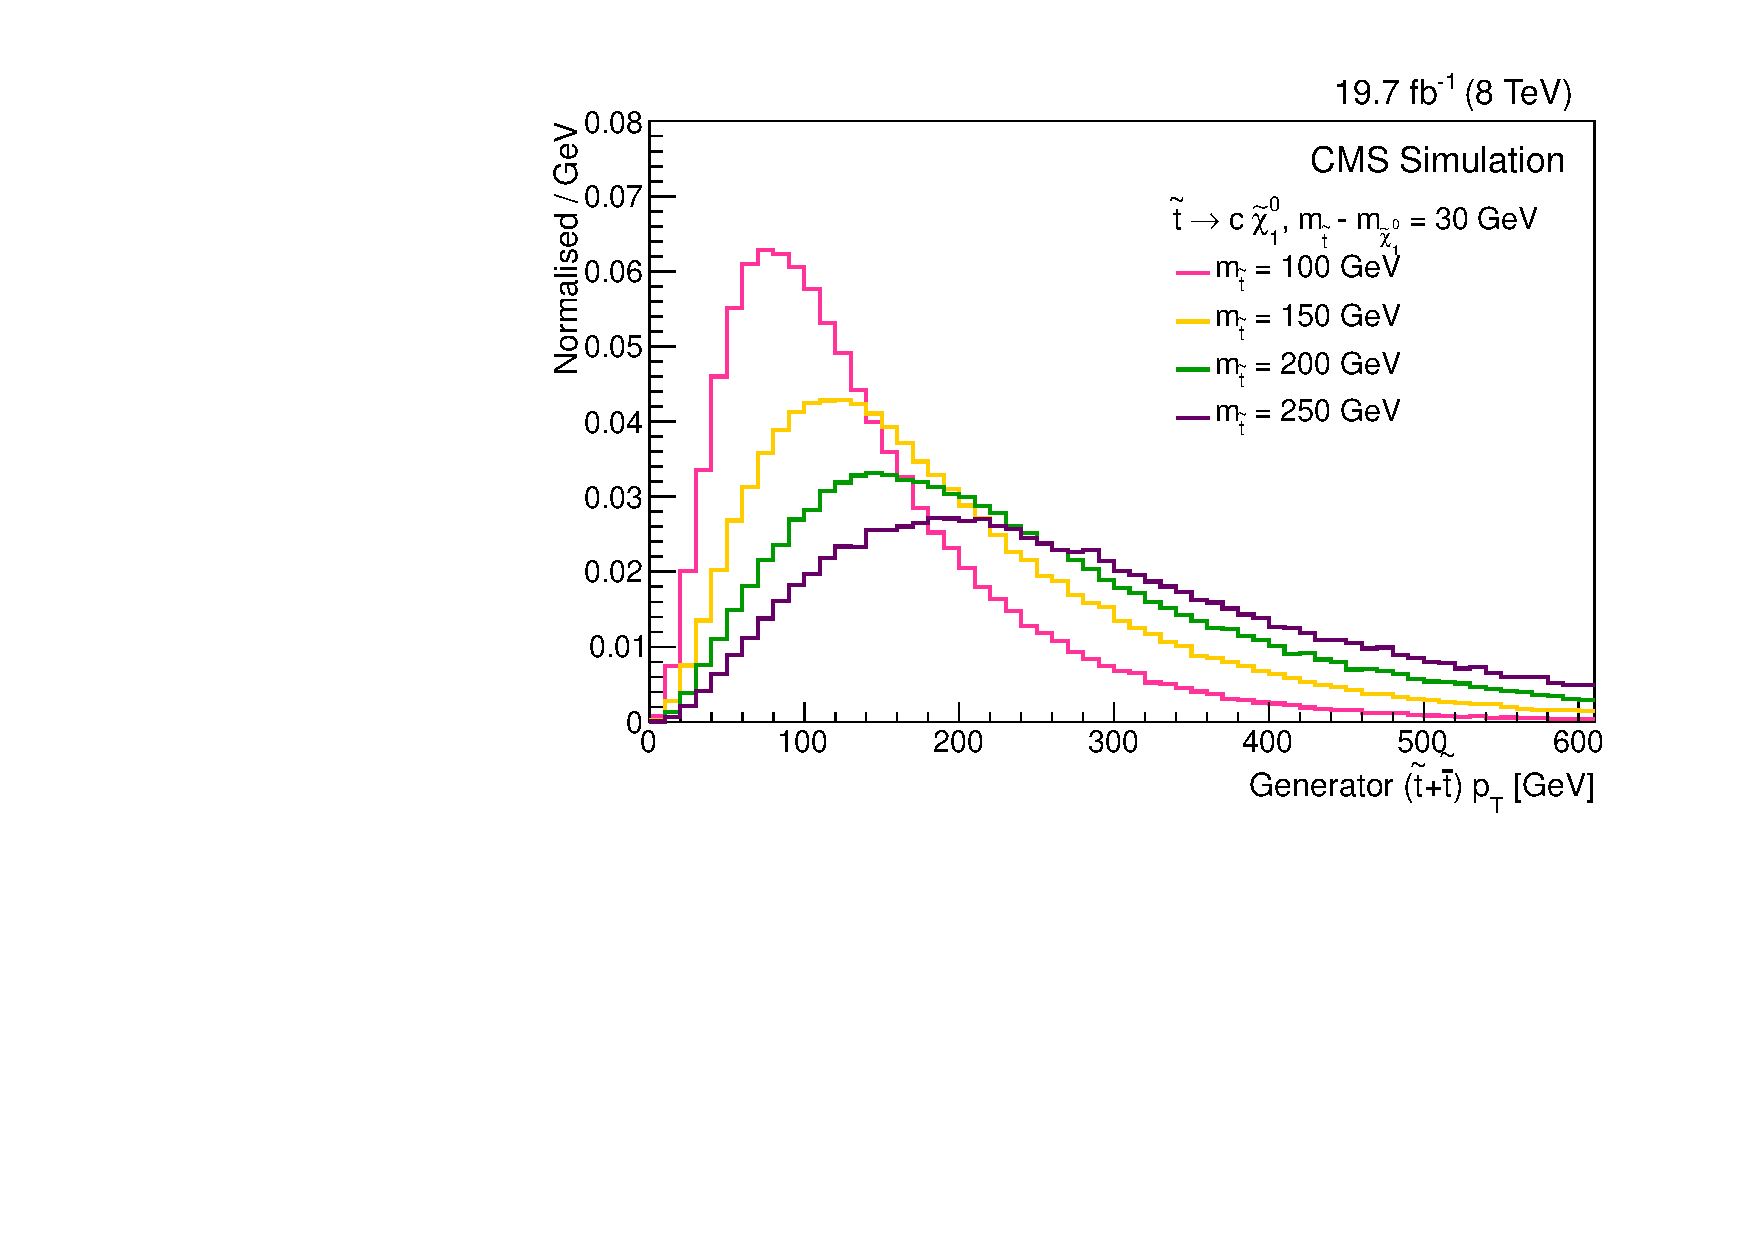
\includegraphics[scale=0.45]{Figures/sus13009/stopstoppt.pdf}
  \caption{Total \pt{} of the $\sTop\santiTop${} pair for various signal hypotheses, where the mass splitting $m_{\sTop}-m_{\chiOneZero} = 30~\GeV$. The $\sTop\santiTop${} system has a larger boost for larger $\sTop${} masses.
         \label{stopstoppT}}
  \end{center}
\end{figure*}


Various kinematic distributions are shown in Figure~\ref{fig:n-1plots}, before selection cuts are applied to that variable.
The corresponding distribution after the cut has been applied is shown in Figure~\ref{fig:nplots}.
Superimposed on the plots in Figure~\ref{fig:nplots} are signal distributions for $\ttwocc$ where $m_{\sTop} = 250~\GeV$ and $m_{\sTop} = 240~\GeV$.
Table \ref{tab:SEL_TabDataMC200} lists the event yields from the various \ac{SM} backgrounds at each step of the analysis, where numbers are taken from simulation and normalized to the integrated luminosity of the data. The cross section used to normalize each background is also listed.

\begin{figure}%[!Hhtb]
  \begin{center}
  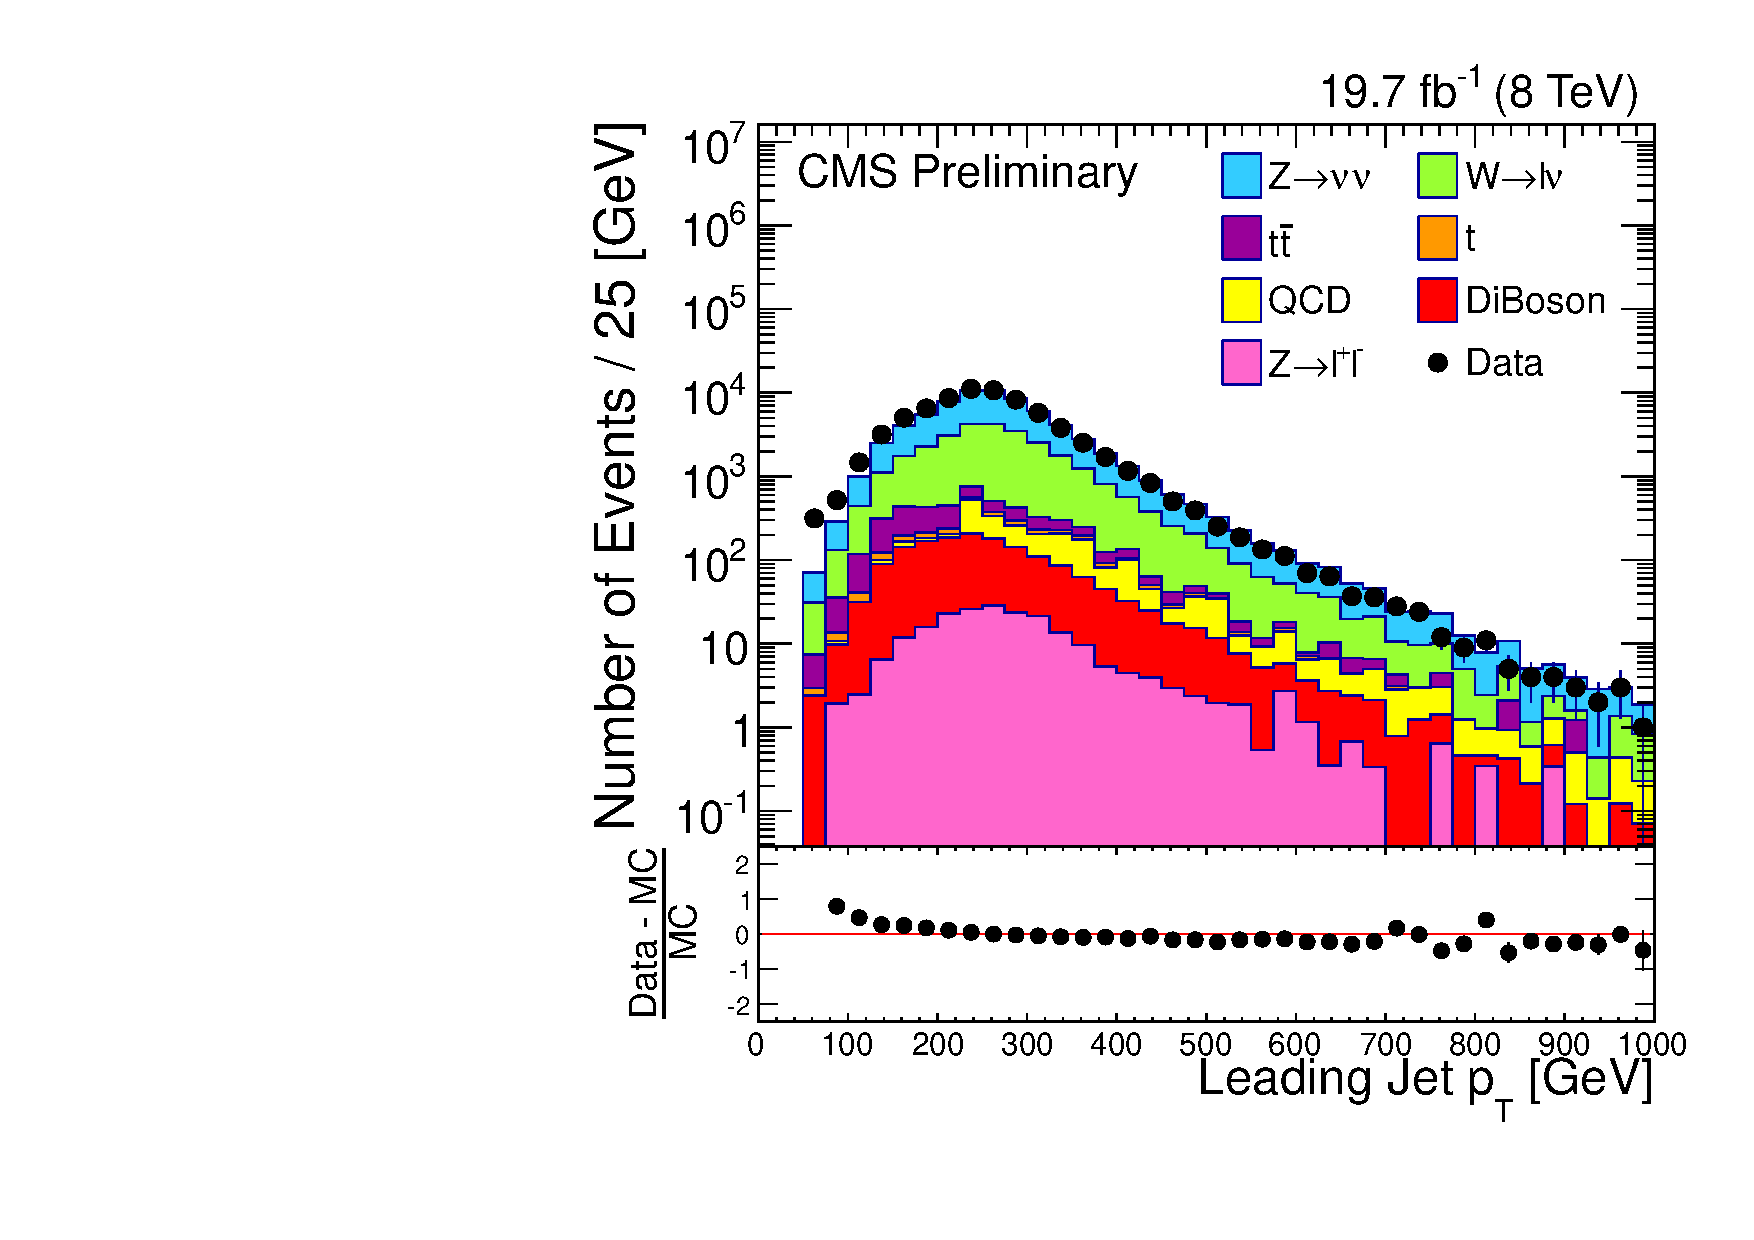
\includegraphics[scale=0.32]     {Figures/sus13009/nocut/Jet1Pt.pdf}
  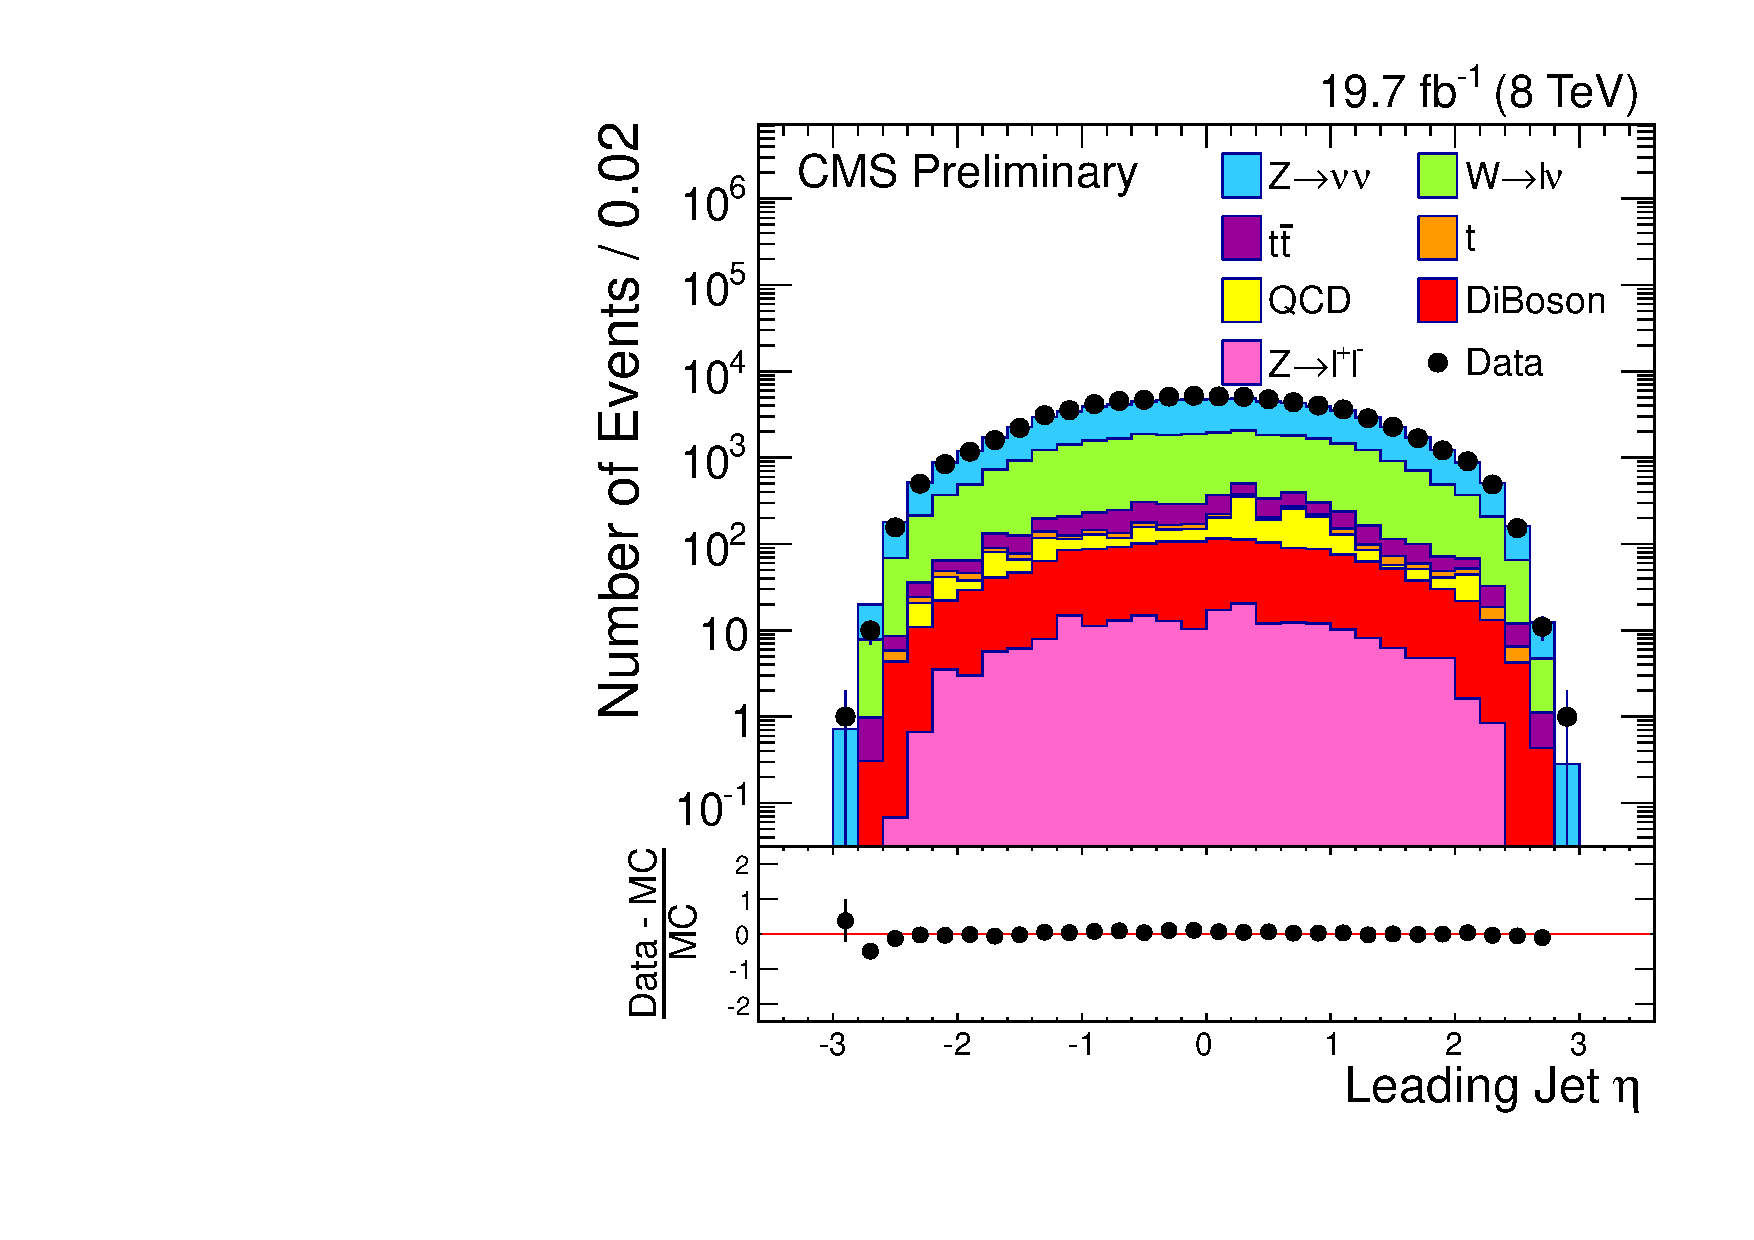
\includegraphics[scale=0.32]     {Figures/sus13009/nocut/Jet1Eta.pdf}
  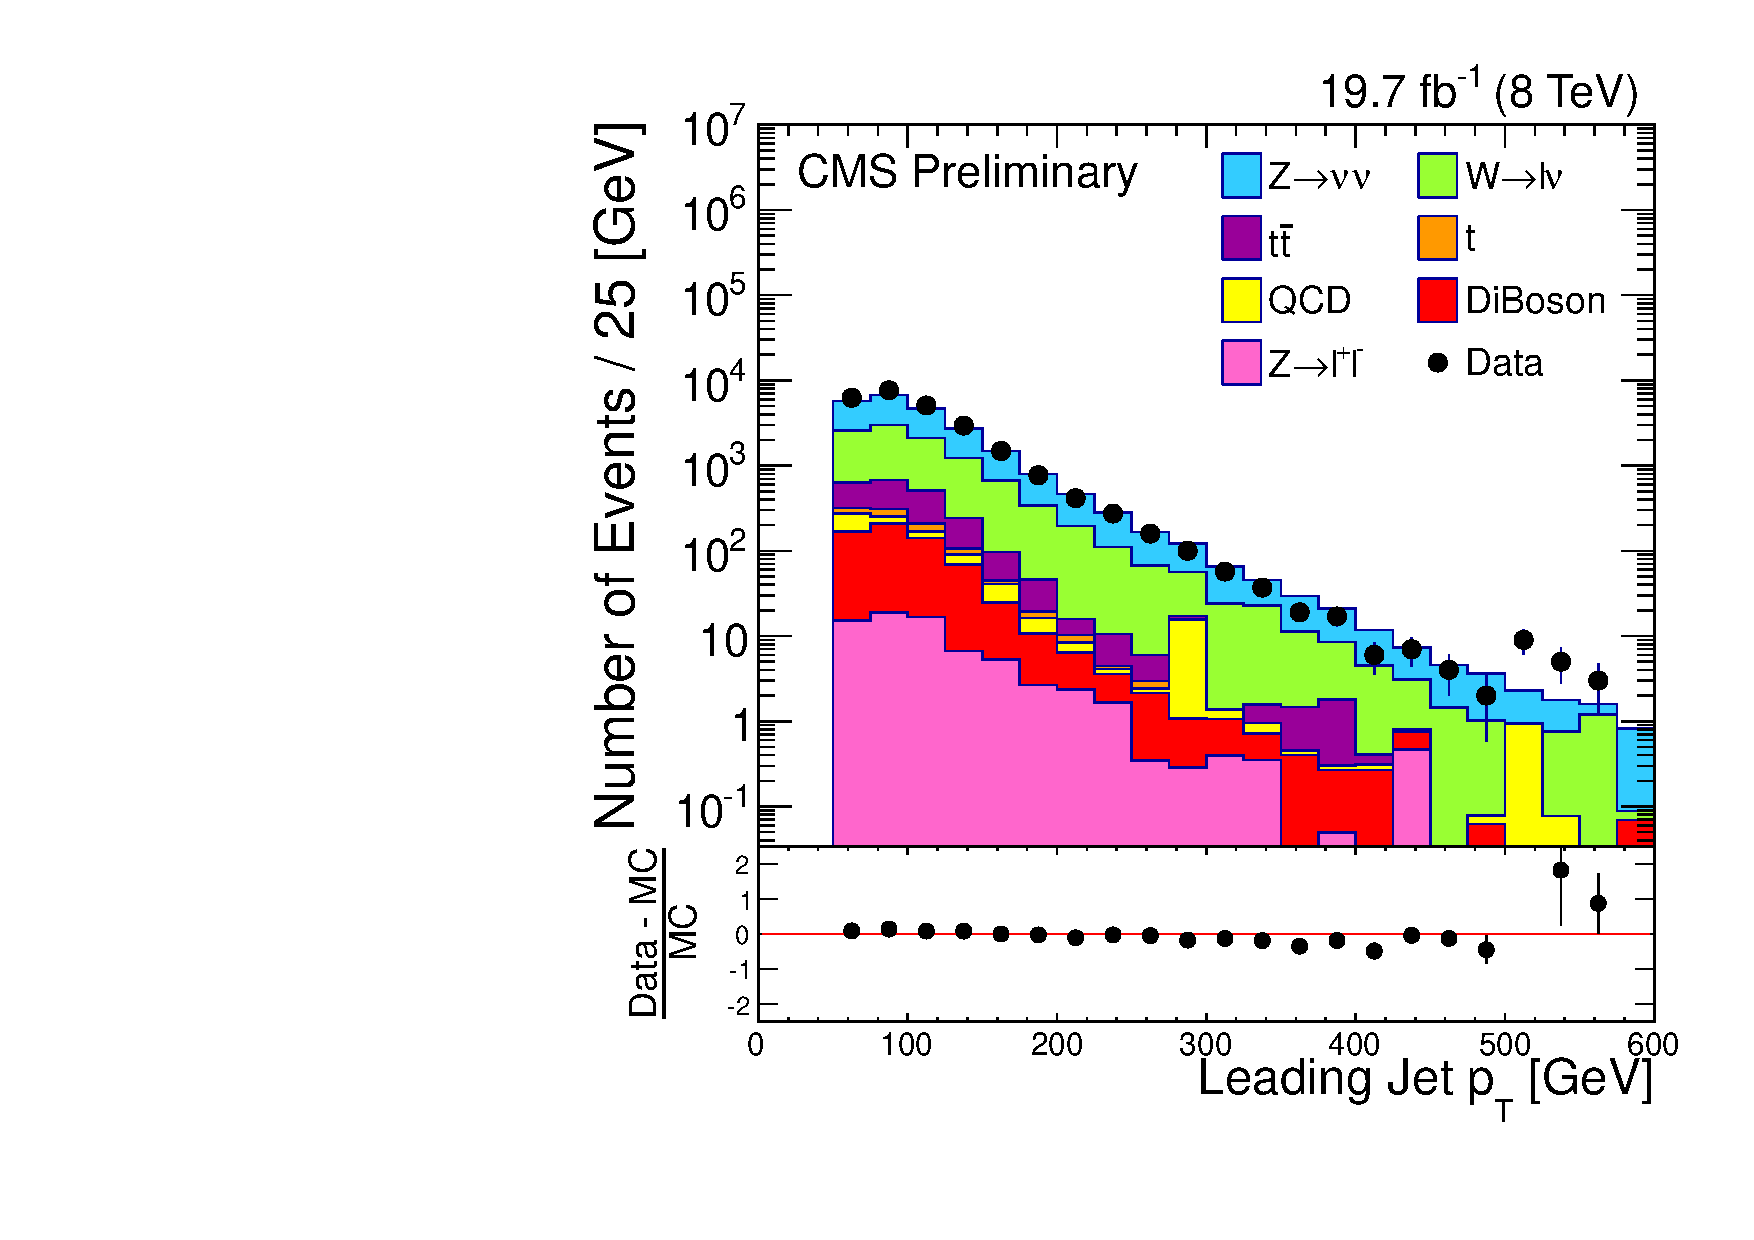
\includegraphics[scale=0.32]     {Figures/sus13009/nocut/Jet2Pt.pdf}
  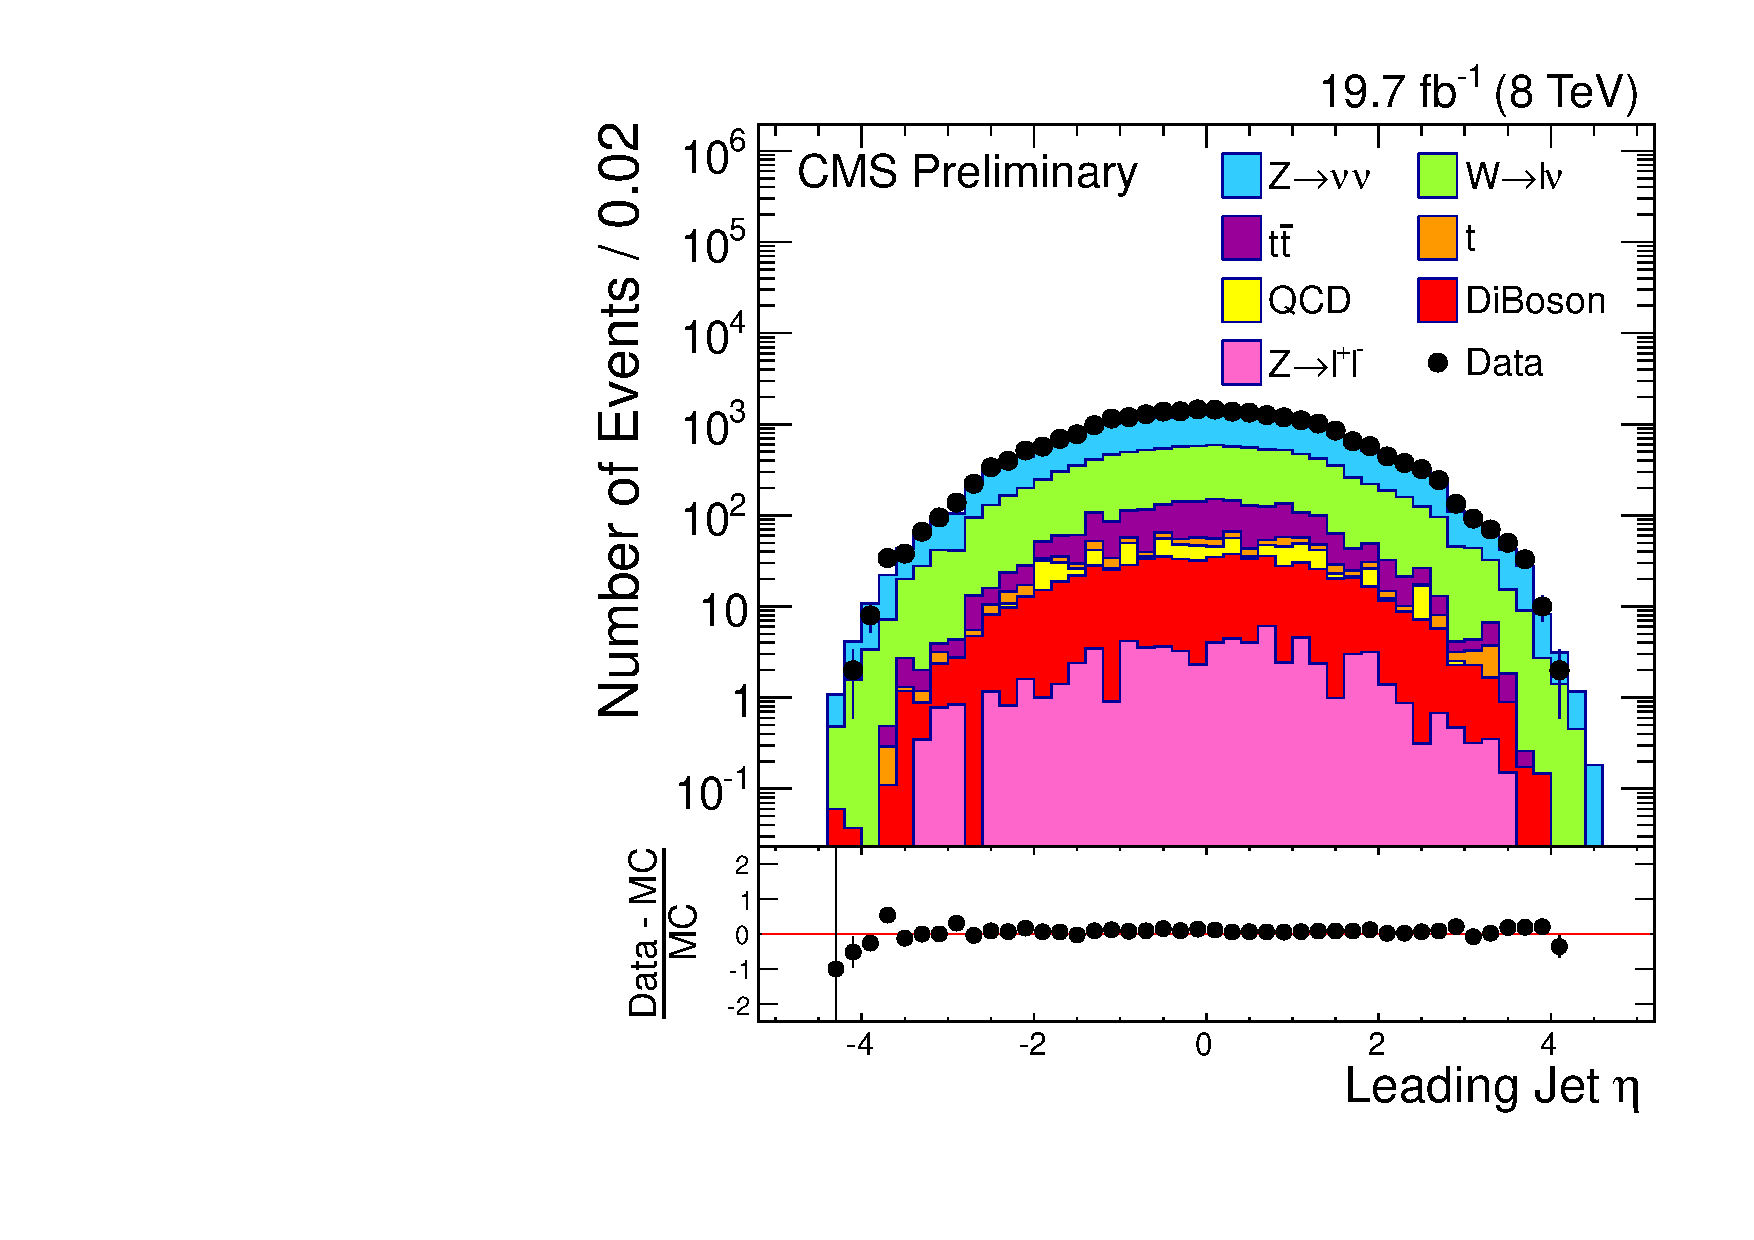
\includegraphics[scale=0.32]     {Figures/sus13009/nocut/Jet2Eta.pdf}
  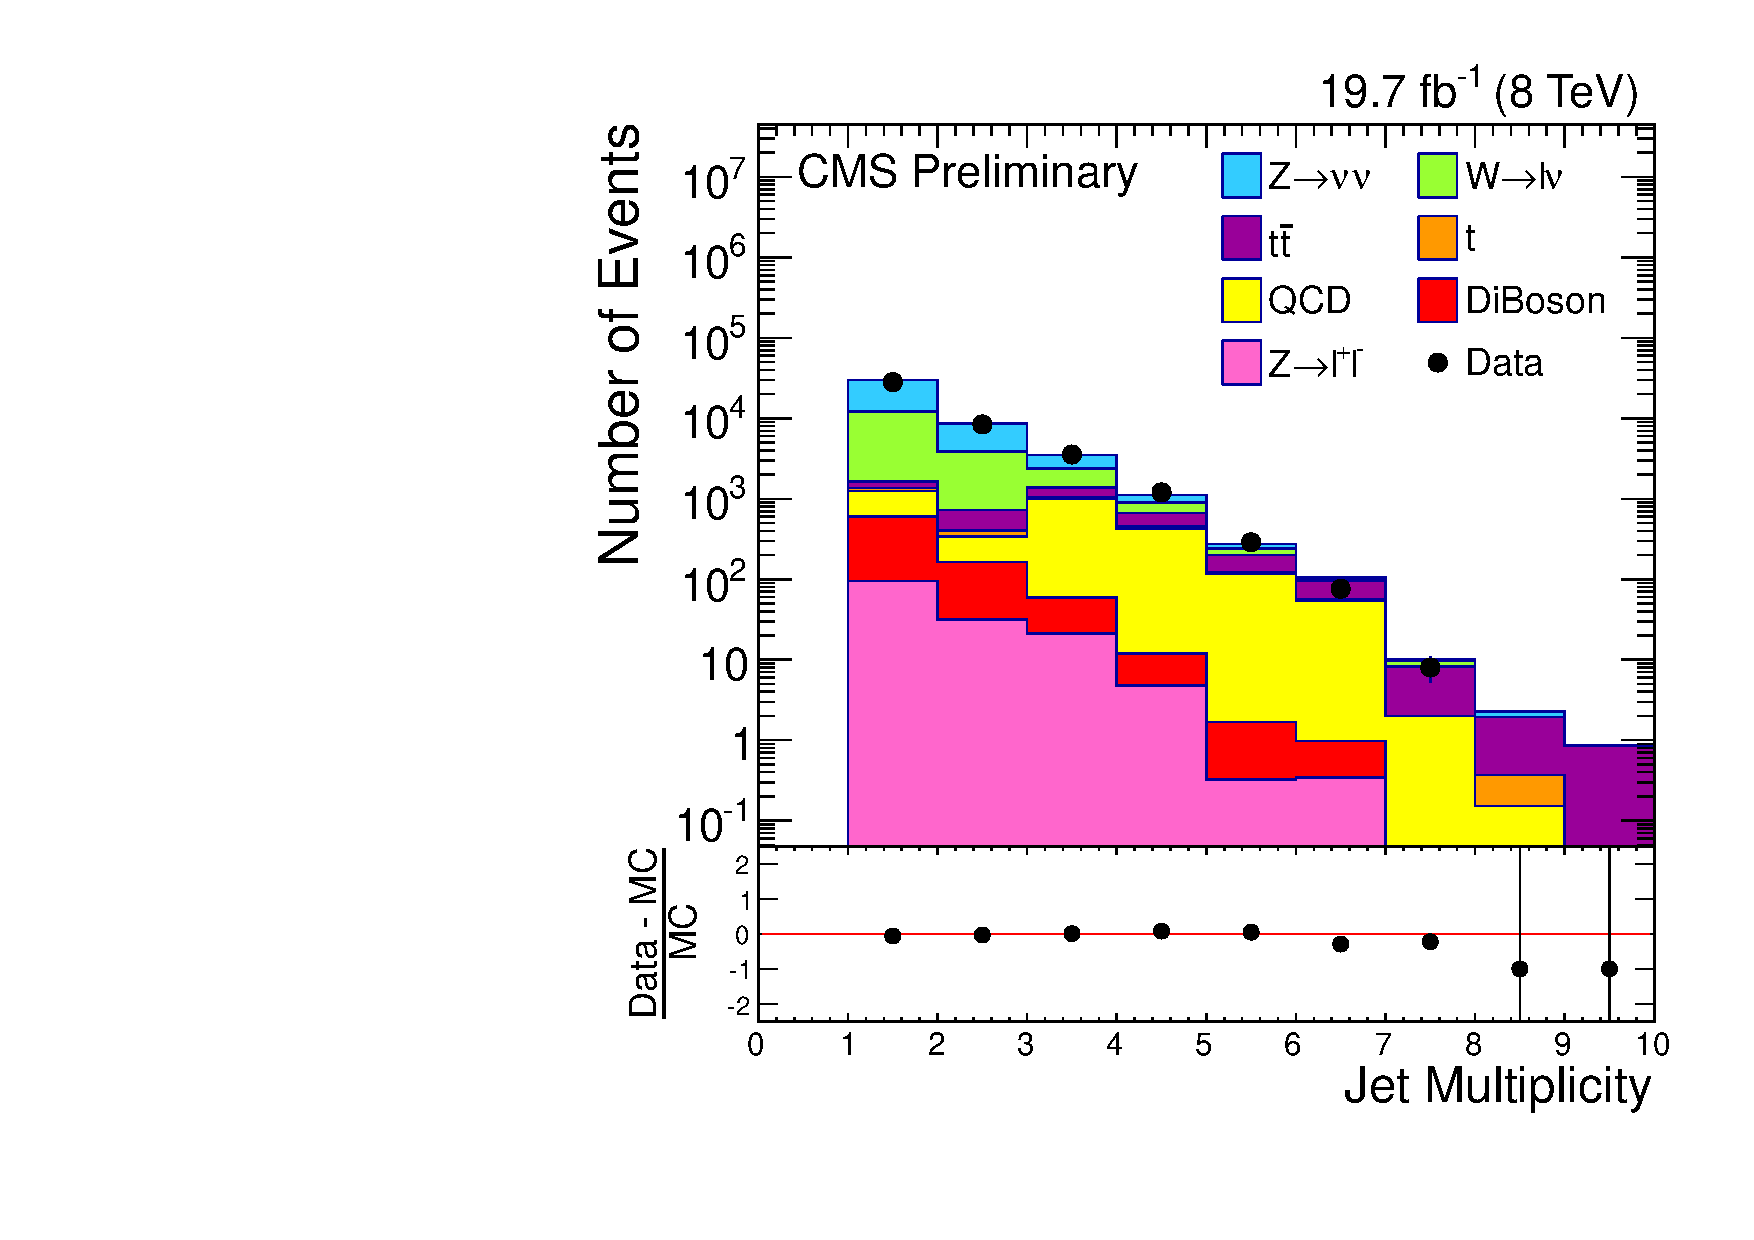
\includegraphics[scale=0.32]     {Figures/sus13009/nocut/NJet.pdf}
  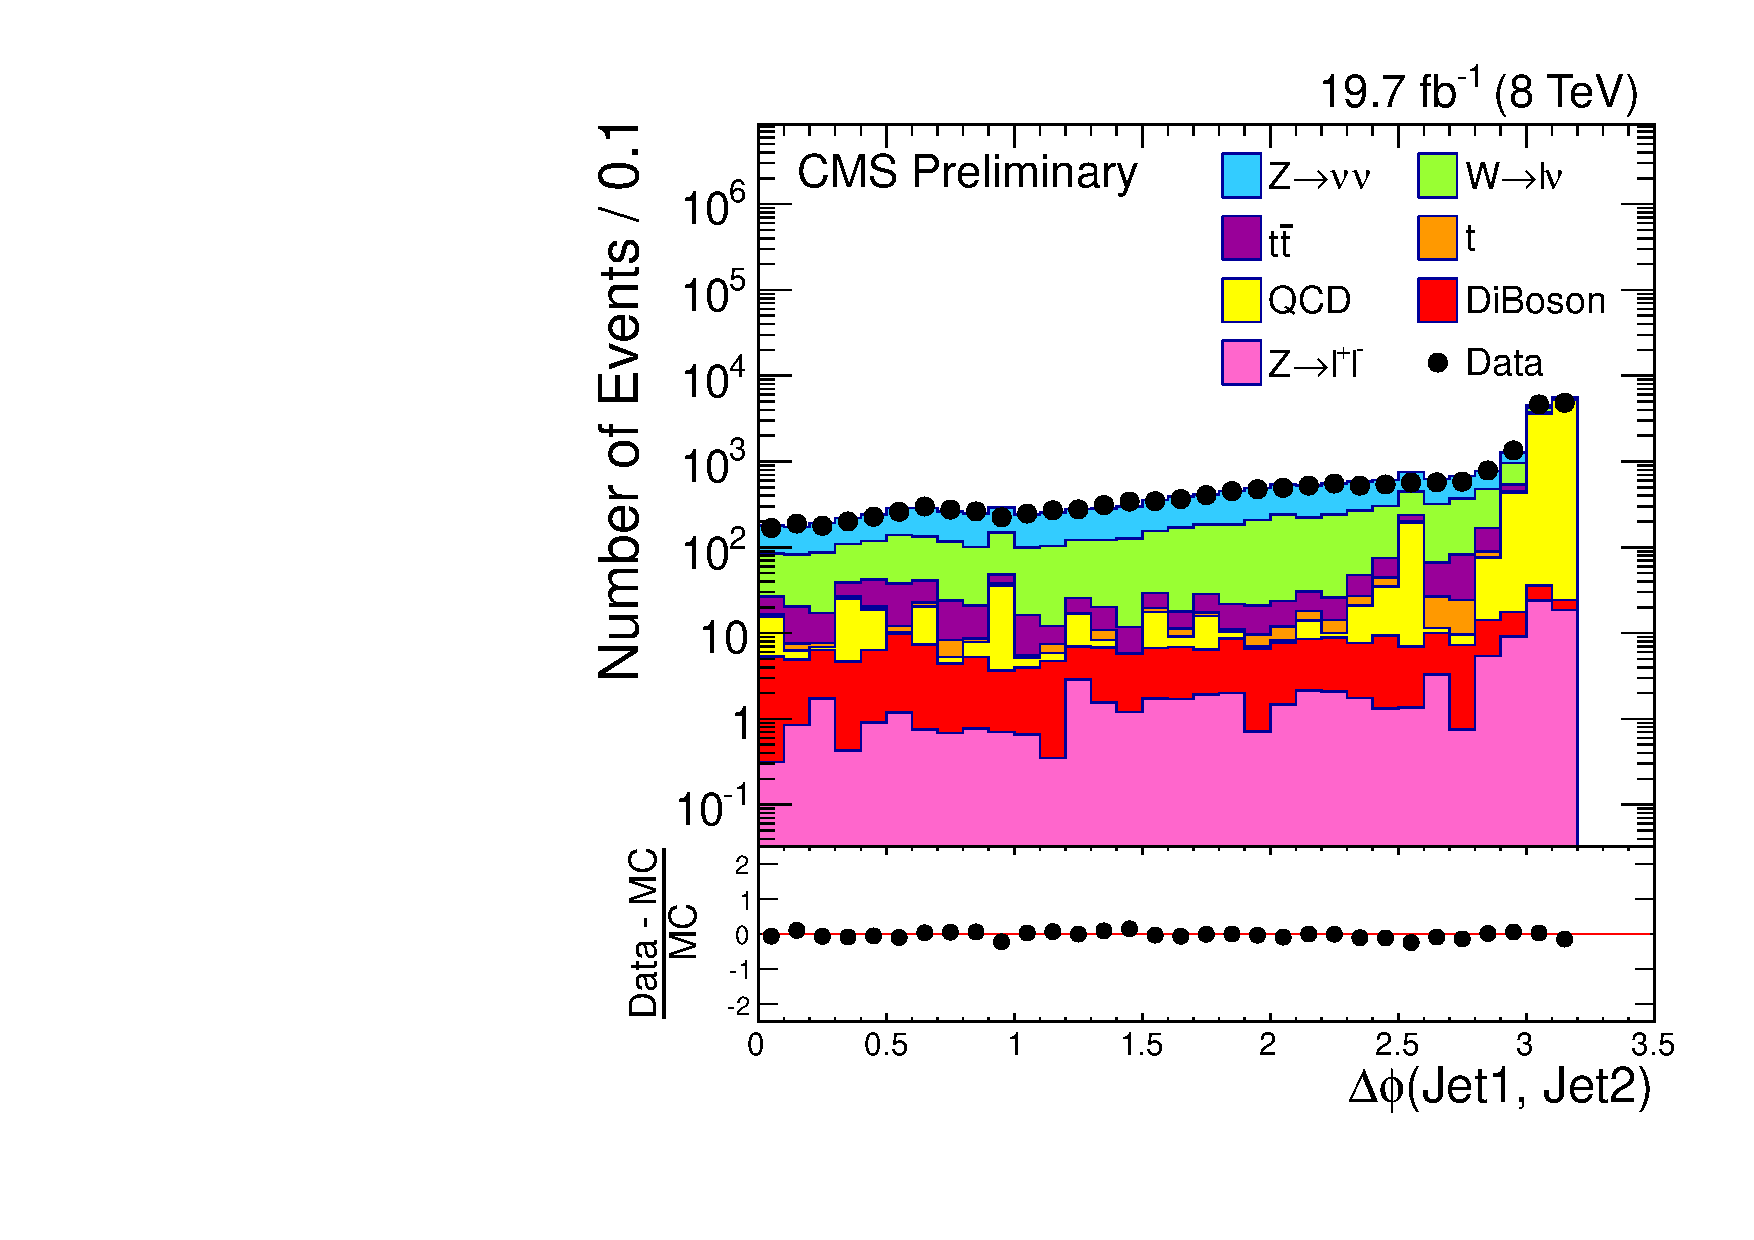
\includegraphics[scale=0.32]     {Figures/sus13009/nocut/dPhi_Jet1_Jet2.pdf}
  \caption{Plots of basic selection variables.  All figures except for the \pt{} and $\eta$ of the second leading jet 
show distributions after all cuts are applied except the one being plotted (the leading jet $\pt$ cut for all plots except the jet $\pt$ and jet $\eta$ is set to 110~\GeV{}). \ac{SM} backgrounds are taken from simulation and normalized to the integrated luminosity using the cross sections shown in Table~\ref{tab:SEL_TabDataMC200}.
  \label{fig:n-1plots}}
  \end{center}
\end{figure}

\begin{figure}%[!Hhtb]
  \begin{center}
  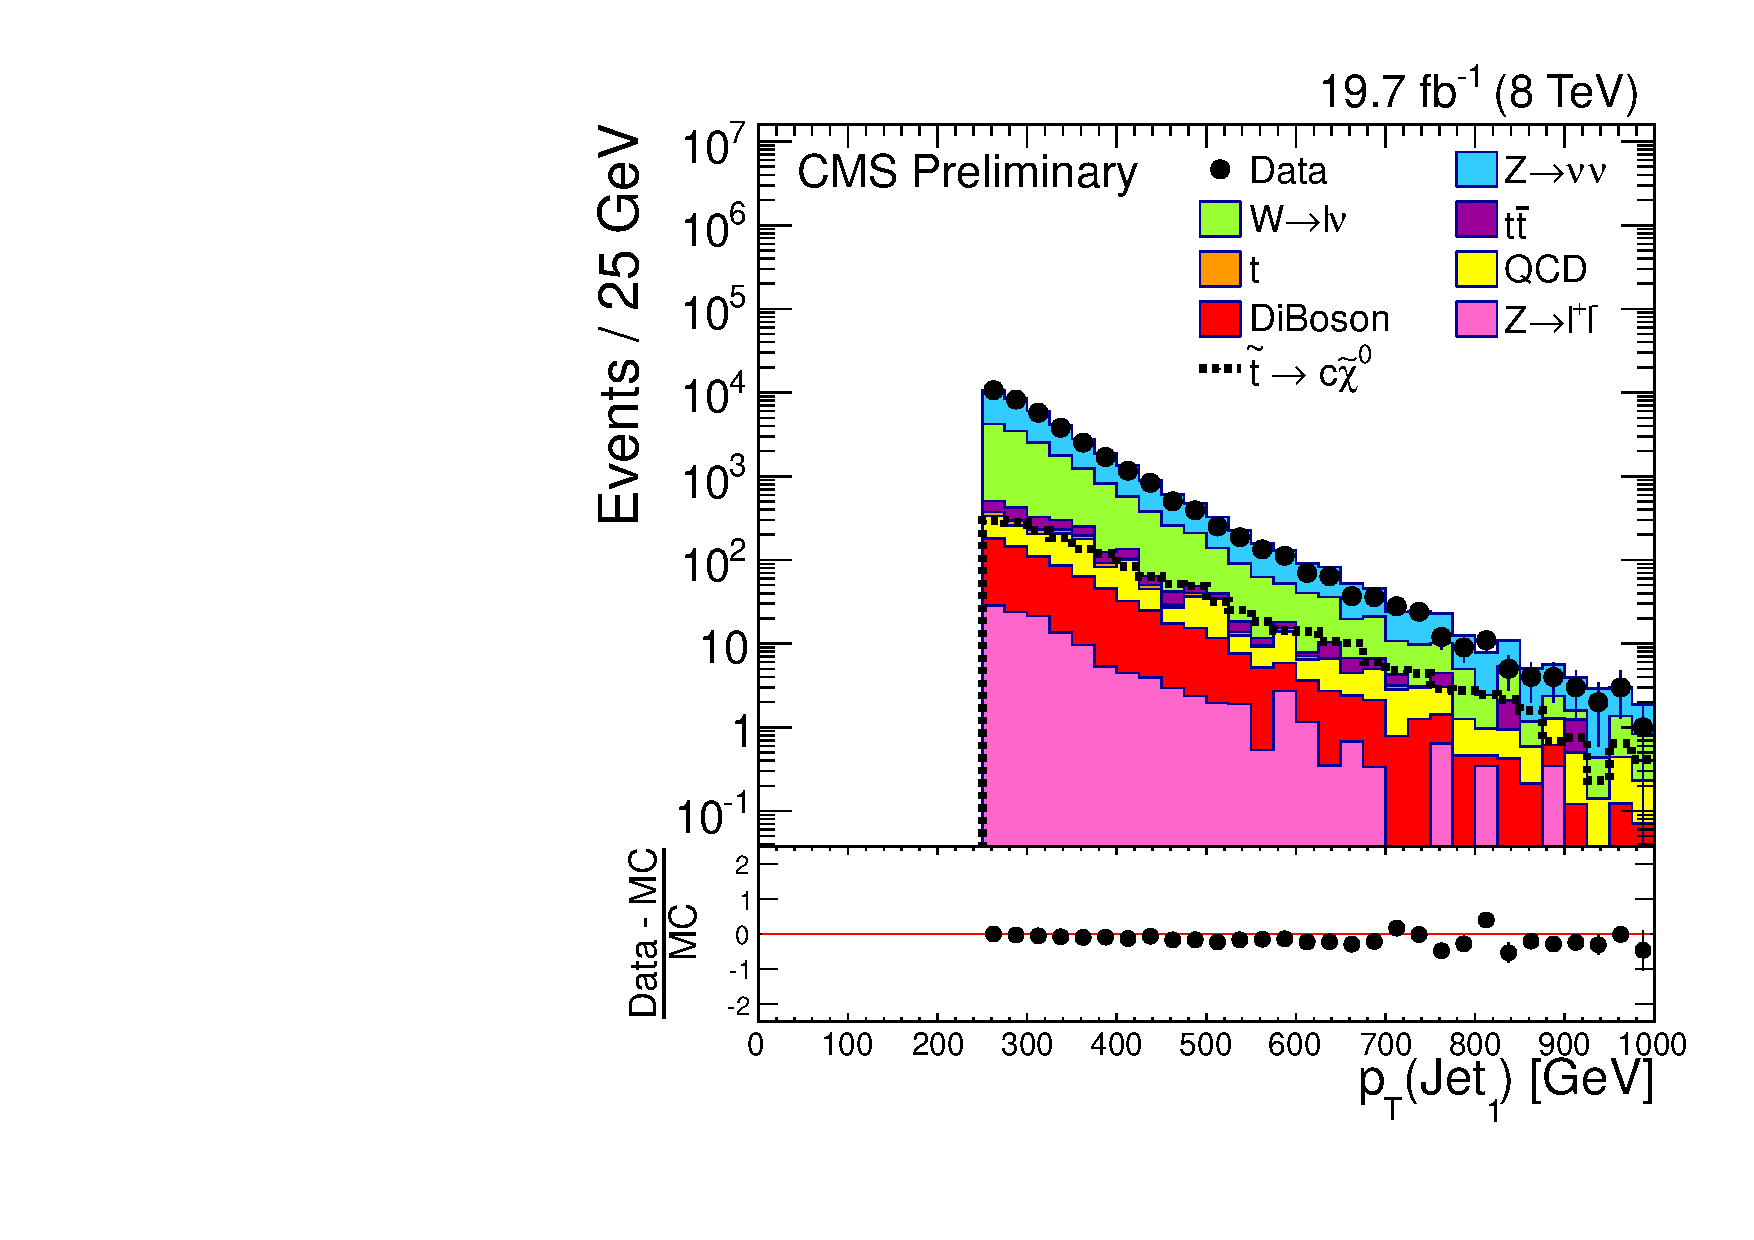
\includegraphics[scale=0.32]     {Figures/sus13009/cut/Jet1Pt.pdf}
  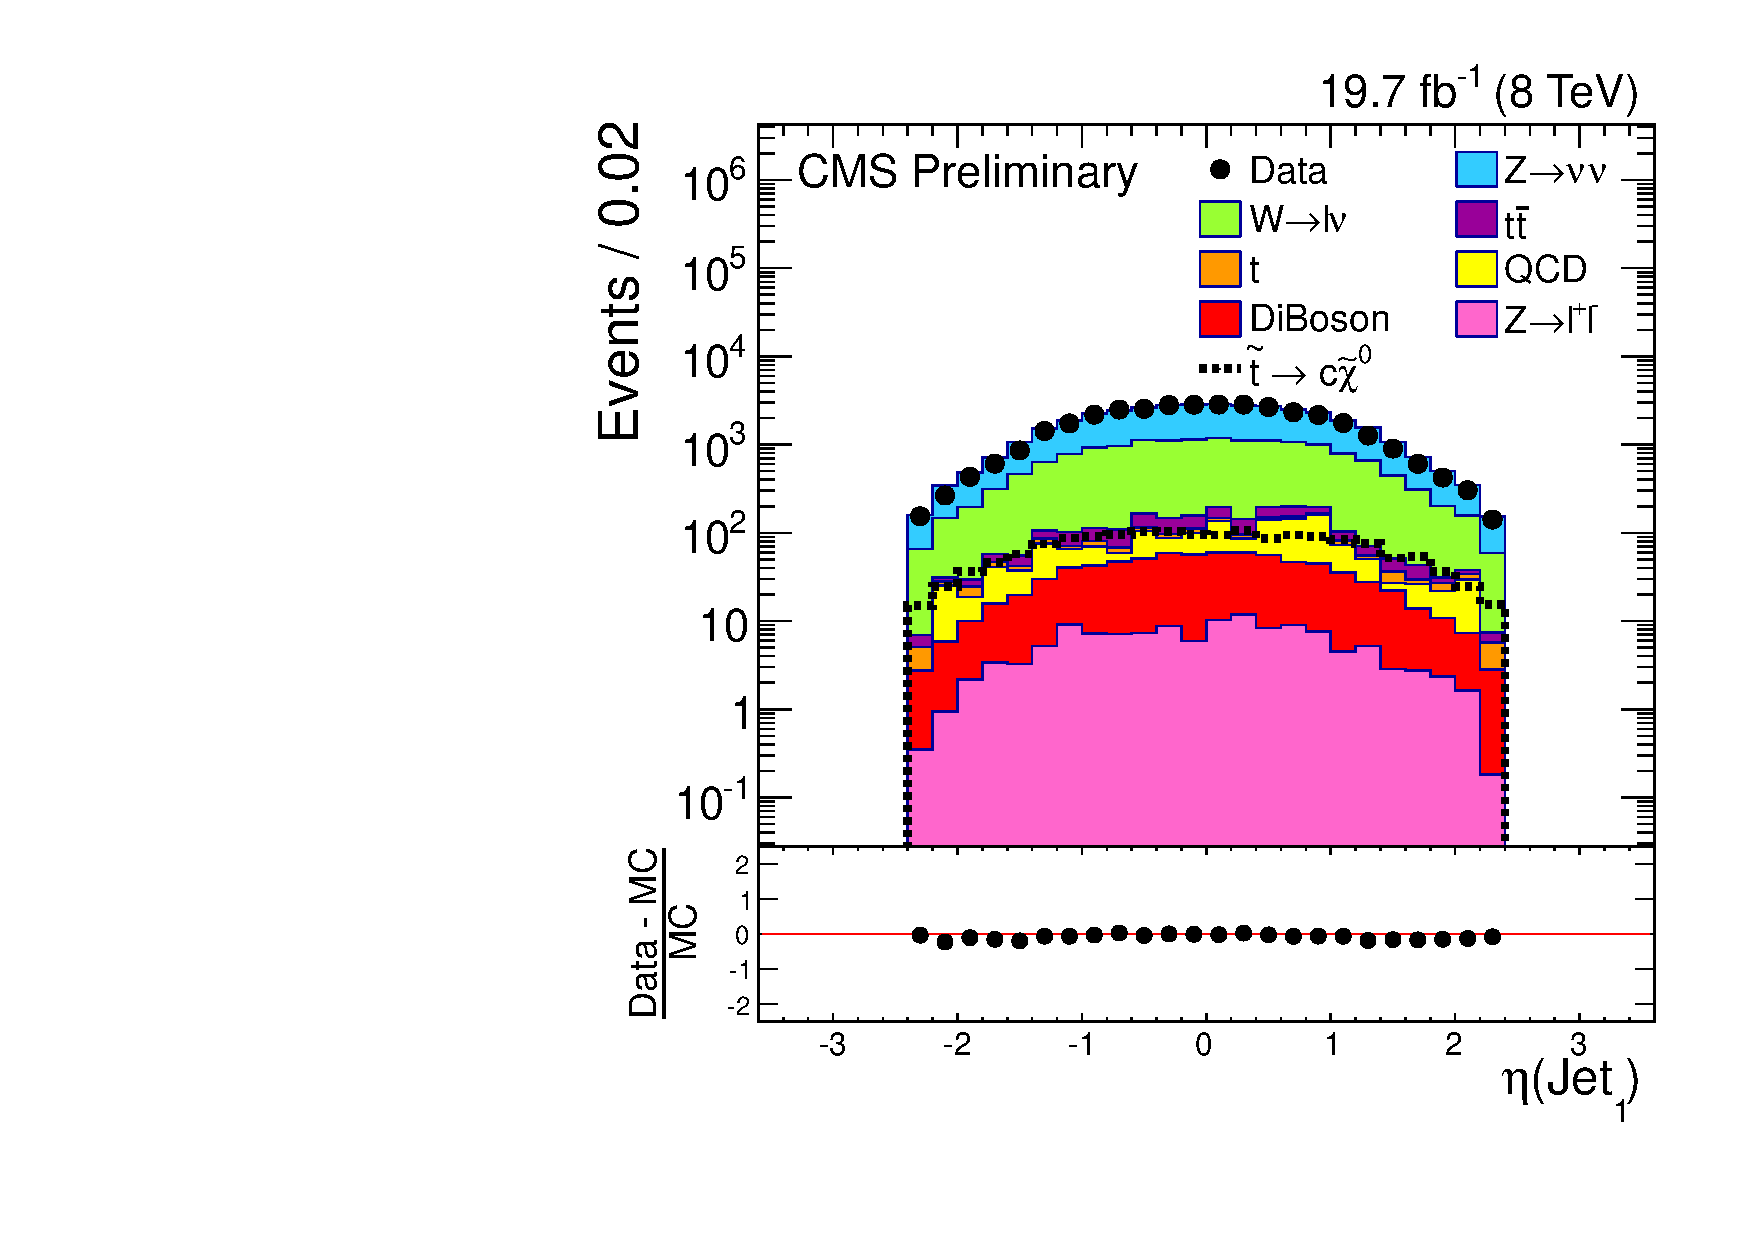
\includegraphics[scale=0.32]     {Figures/sus13009/cut/Jet1Eta.pdf}
  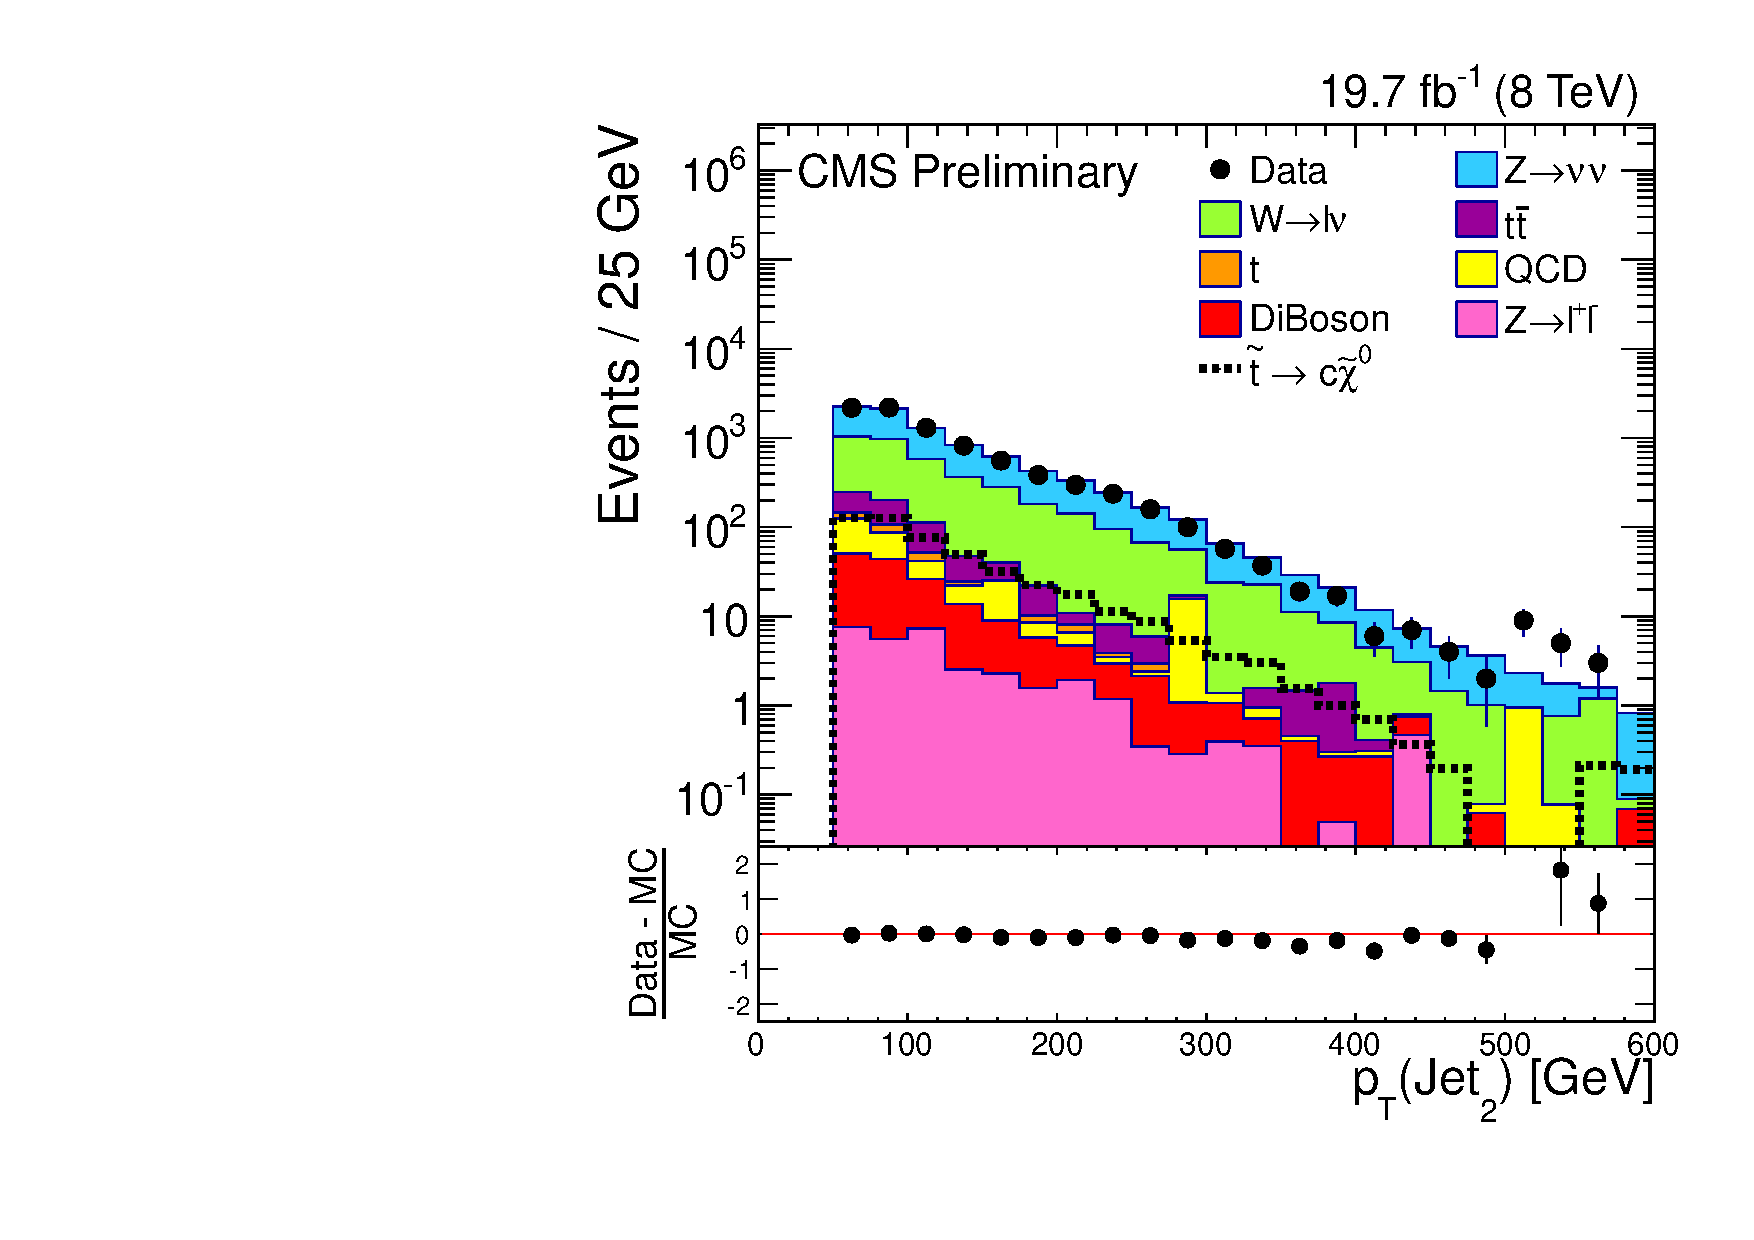
\includegraphics[scale=0.32]     {Figures/sus13009/cut/Jet2Pt.pdf}
  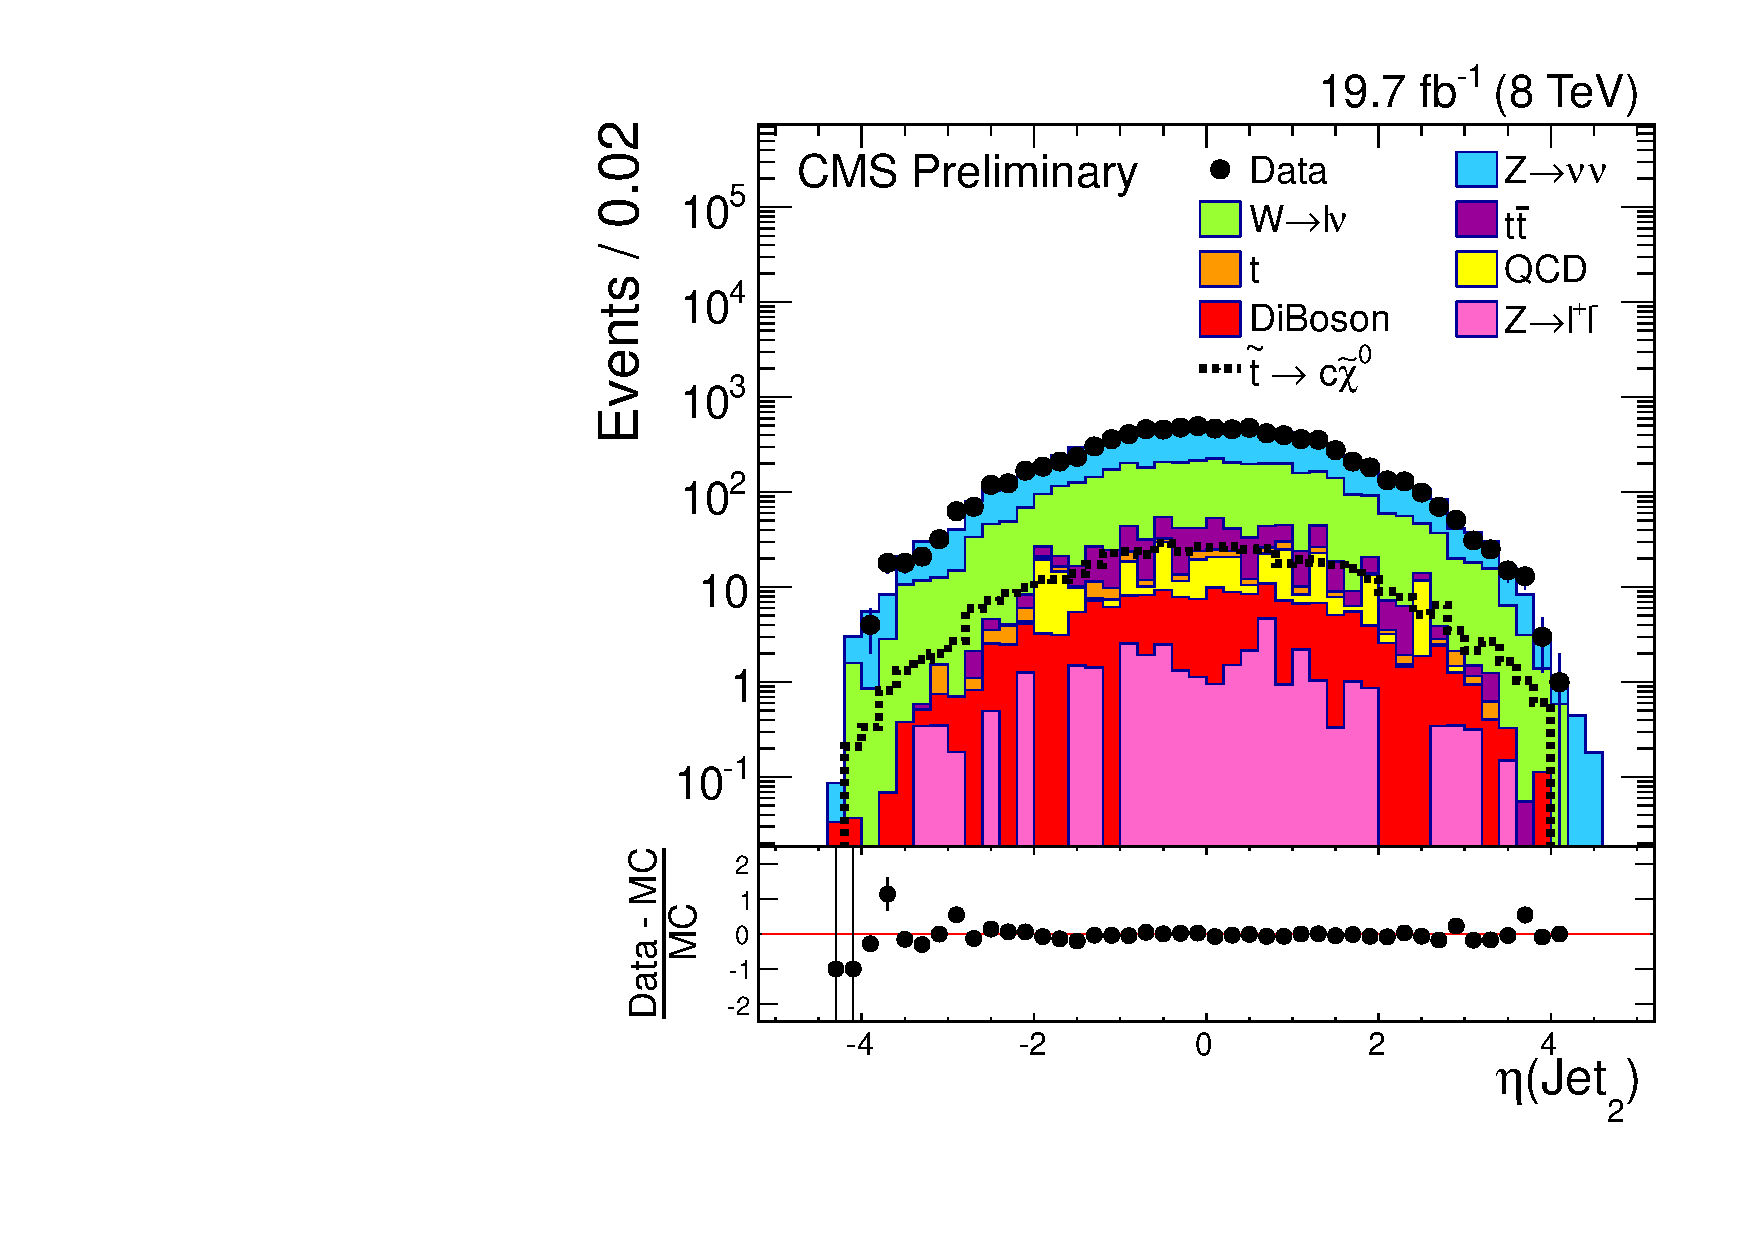
\includegraphics[scale=0.32]     {Figures/sus13009/cut/Jet2Eta.pdf}
   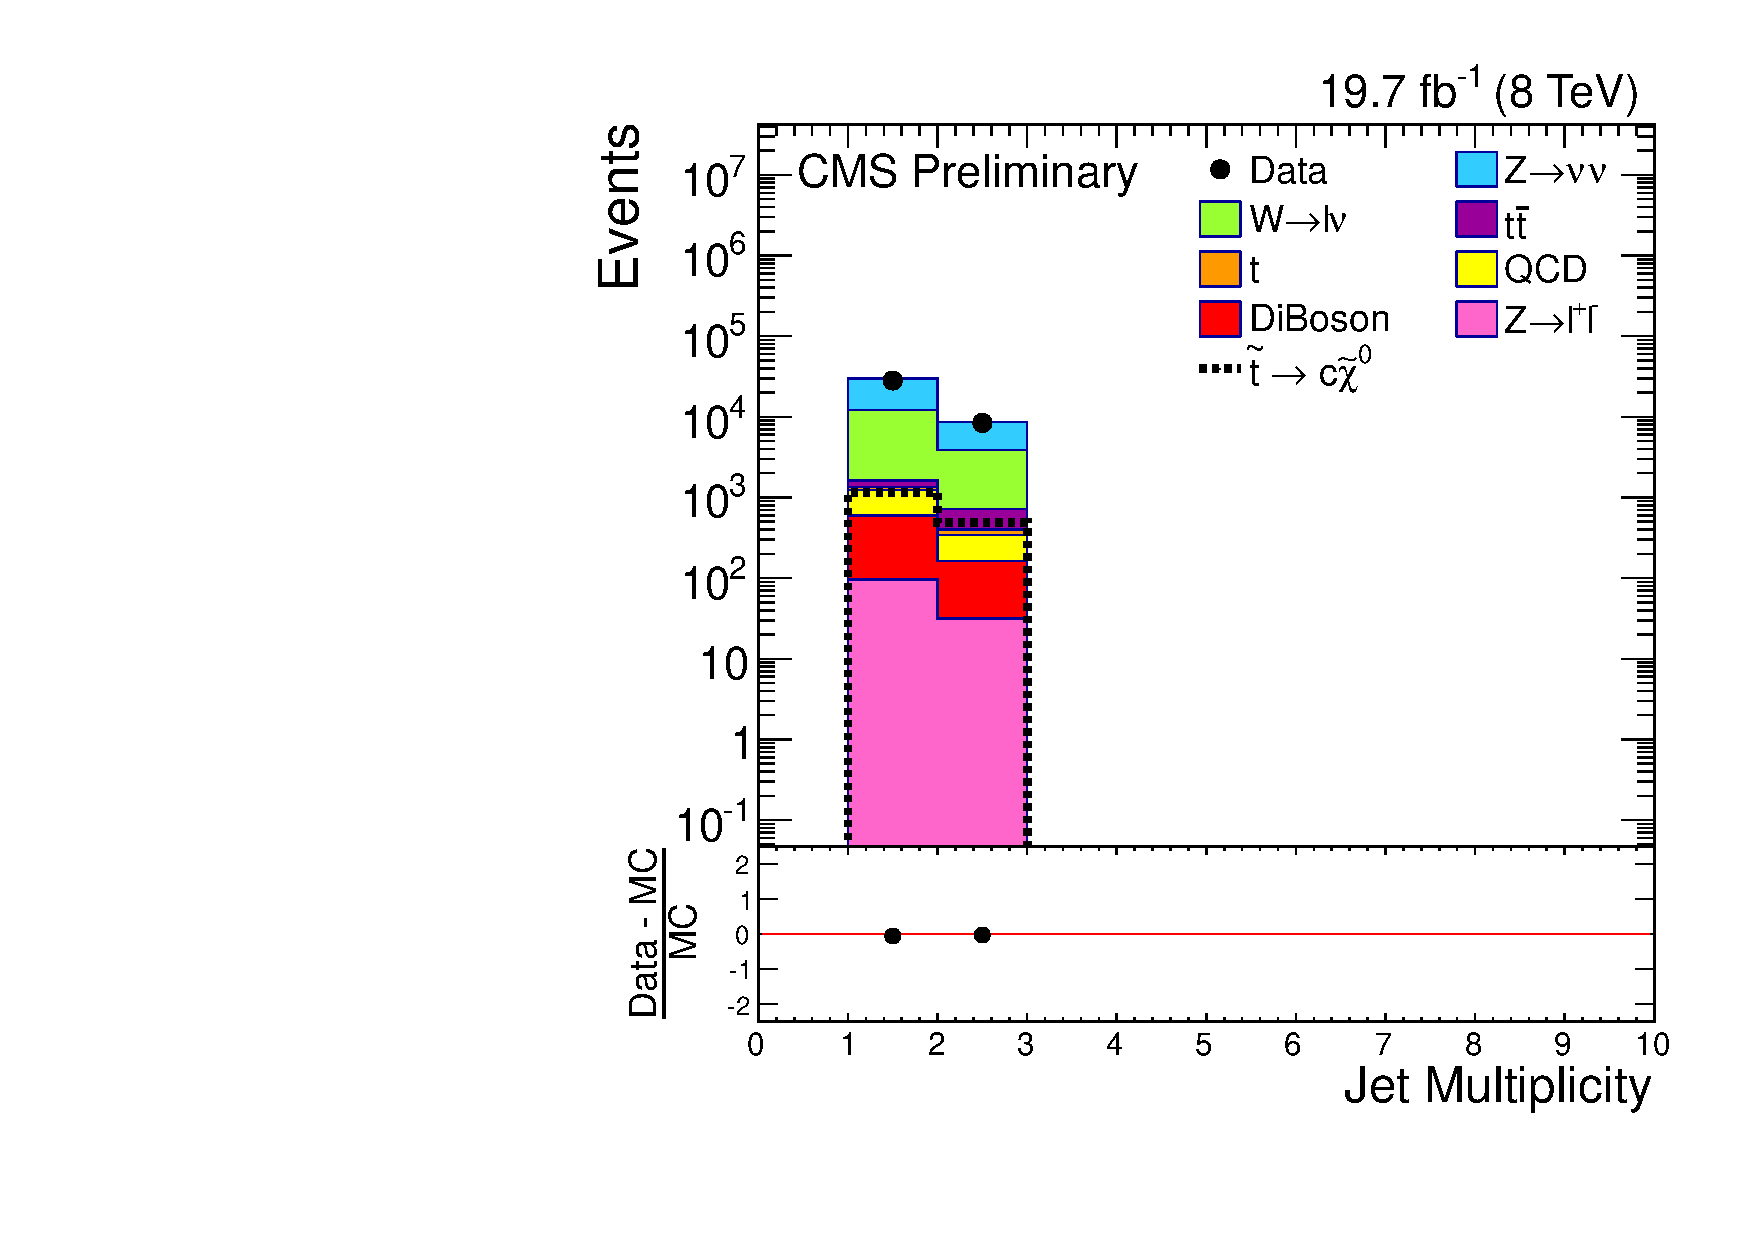
\includegraphics[scale=0.32]     {Figures/sus13009/cut/NJet.pdf}
   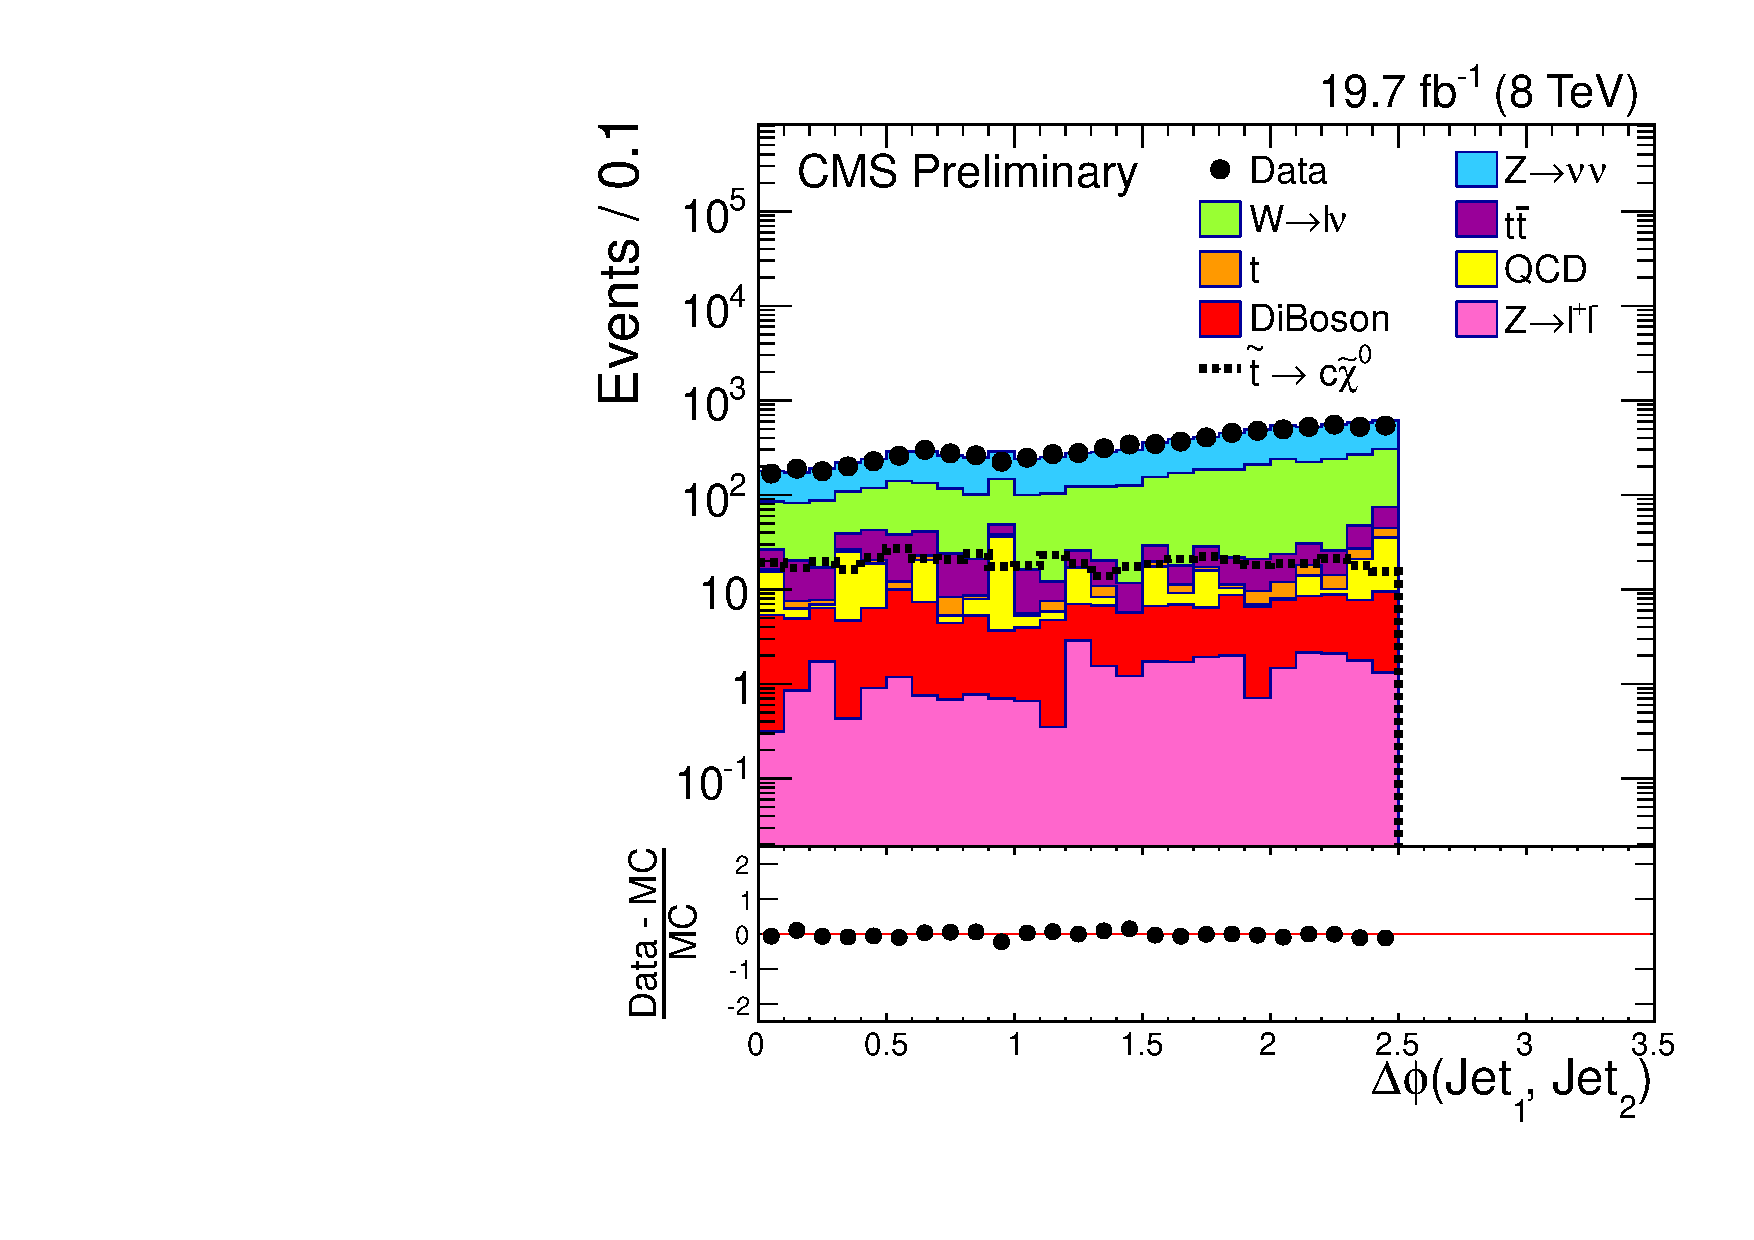
\includegraphics[scale=0.32]     {Figures/sus13009/cut/dPhi_Jet1_Jet2.pdf}
   \caption{Plots of selection variables in the baseline search region, where $\pt(\jet_1)>250~\GeV$. \ac{SM} backgrounds are taken from simulation. Superimposed are kinematic distributions for the signal $\ttwocc$ where $m_{\sTop} = 250~\GeV$ and $m_{\sTop} = 240~\GeV$. 
   Distributions of \ac{SM} processes and signal are taken from simulation and normalised to the integrated luminosity of the dataset.
         \label{fig:nplots}}
  \end{center}
\end{figure}


%Fig.~\ref{fig:ANA_Jet_selection_plots} where the full monojet selection has been applied with a $\MET$ cut of 250 \GeV. All the distributions have been normalised as described in Appendix~\ref{app:normalisation}.

%The distribution of \MET for data and background after selecting monojet events and for a \MET cut of 250 \GeV{} is shown in Figure~\ref{fig:ANA_MET_plots}.

%We define the above described event selection with the \MET cut of 200 GeV as the baseline selection and subsequently apply tighter \MET\ selections of $\MET = 250, 300, 350, 400$ to obtain our search regions. 
%Optimisation studies have been performed for each of our signal samples to find the value of the \MET\ cut that gives the best expected limit. The study is documented in Appendix~\ref{app:opt_limit}. For both the ADD and dark matter signal points, the optimal \MET\ cut is found to be 350 \GeV. For Unparticles, the optimal \MET cut is found to be 300 \GeV{} or 350 \GeV, depending on the values of $d_U$. However the difference in expected limit is small and therefore a \MET\ cut of 350 \GeV{} is used for calculating limits, consistent with what is used for the ADD and dark matter signals.
%
%\begin{figure}[tb]
%  \begin{center}
%  \includegraphics[scale=0.45]{cut/Met.pdf}
%  \caption{The $\MET$ distribution after all selection cuts are applied for data and backgrounds.Representative signal distributions for dark matter, ADD and Unparticles are also overlaid. Events with $\MET > 1 \TeV$ are included in the overflow bin.}
%         \label{fig:ANA_MET_plots}  
%  \end{center}
%\end{figure}

\newsavebox{\cutflowBoxa}
\begin{table*}[htb] %table 7 v04 110811:05  
        \begin{center}
        \caption{For illustrative purposes, event yields from different simulated samples for the \ac{SM} backgrounds at each step of the event selection including the search regions. 
        Backgrounds are obtained directly from simulation and normalized to an integrated luminosity of 19.7~\fbinv using the cross sections shown in the table.}
\label{tab:SEL_TabDataMC200}
 {\footnotesize
         \begin{lrbox}{\cutflowBoxa}
               \begin{tabular}{l|ccccccc|c} \hline
Selection     & \wpj & \zellellbr{}\,+\,jets & \znunubr{}\,+\,jets & Diboson &  $\ttbar$ &  Single-top &  QCD multijet & Total BG   \\ \hline 
Cross section (pb) & 228.9  & 40.5   & 588.3  & 234.0  & 1.085e6  & 114.8  & 105.7  &   \\ \hline
%Generated events   & 1.27e7 & 2.66e6 & 1.45e7 & 6.86e6 & 4.27e7   & 7.06e6 & 2.98e7 &   \\ \hline
Event cleaning                 & 2514352 &  190332   & 4337526 &  65666  & 461413 & 77284 &  5429269 &  13075841 \\ 
$\METmu >200$ \GeV{}               & 317656  &  30242    & 134578  &  9572   & 63174  & 9289  &  87605   &  652117   \\
Noise cleaning                 & 292550  &  27880    & 123420  &  8706   & 59412  & 8525  &  81668   &  602162   \\
$\pt(\,\mathrm{j}_1)>$110~\GeV{} & 279323  &  26652    & 117513  &  8045   & 53353  & 7752  &  80844   &  573484   \\ 
$\njets \le 2$      	         & 254058  &  24413    & 109313  &  7287   & 29364  & 5596  &  44247   &  474278   \\ 
$\Delta\phi(\jet_1,\jet_2)<2.5$& 237533  &  22947    & 104158  &  6984   & 25312  & 4815  &  8433    &  410181   \\ 
$\mu$ veto                     & 106236  &  1511     & 104152  &  4051   & 9826   & 1892  &  7444    &  235112   \\ 
$e$ veto                       & 79407   &  1004     & 104065  &  3459   & 6557   & 1325  &  7401    &  203218   \\ 
\tauh veto                     & 71808   &  807      & 103106  &  3248   & 5599   & 1147  &  7047    &  192762   \\ \hline 
$\pt(\,\mathrm{j}_1)>250$~\GeV{} 
& \multirow{2}{*}{13641}
& \multirow{2}{*}{127}   
& \multirow{2}{*}{22615}
& \multirow{2}{*}{639}
& \multirow{2}{*}{602}
& \multirow{2}{*}{172}
& \multirow{2}{*}{819}
& \multirow{2}{*}{38615}    \\
               \,\,\& $\METmu>250$~\GeV{}   &        &           &          &         &         &        &           &           \\
$\pt(\,\mathrm{j}_1)>300$~\GeV{}   &6873    &  75       &11093     & 369     & 344     & 97     &  546      &  19397   \\ 
$\pt(\,\mathrm{j}_1)>350$~\GeV{}   &3182    &  40       &5231      & 206     & 178     & 49     &  332      &  9218    \\ 
$\pt(\,\mathrm{j}_1)>400$~\GeV{}   &1501    &  25       &2617      & 113     & 91      & 21     &  181      &  4549    \\ 
$\pt(\,\mathrm{j}_1)>450$~\GeV{}   &751     &  17       &1335      & 64      & 48      & 11     &  92       &  2318    \\ 
$\pt(\,\mathrm{j}_1)>500$~\GeV{}   &376     &  11       &727       & 36      & 27      & 5.2    &  61       &  1244    \\ 
$\pt(\,\mathrm{j}_1)>550$~\GeV{}   &204     &  7.4      &406       & 21      & 18      & 3.2    &  34       &  693     \\ \hline 
\end{tabular}
\end{lrbox}
\scalebox{0.80}{\usebox{\cutflowBoxa}}} 
\end{center}
\end{table*}



\section{Background estimation and systematic uncertainties}
\label{sec:BKG}

As is evident in Table~\ref{tab:SEL_TabDataMC200}, the dominant backgrounds in the search regions after the monojet event selection are expected to be electroweak backgrounds.
The largest contribution is due to invisible \Z{} boson decays, \znunubr{}\,+\,jets, which is irreducible as the neutrinos mimic the \ac{LSP}s and there is genuine \MET in the final state. 
The secondary background is due to leptonic \W{} boson decay, \wlnubr{}\,+\,jets, where the lepton (electrons and muons, including those from leptonically decaying taus) is not reconstructed, outside of the kinematic acceptance of the lepton vetoes or not isolated.
Both of these backgrounds are estimated from data by selecting a control sample of $\mu$+jet events, where \zmumubr{}\,+\,jets events are used to predict the invisible Z background and \wmunubr{}\,+\,jets events are used to predict the \wlnubr{}\,+\,jets background.
Small contributions from \ac{QCD} multijet and \ttbar{} events are estimated using simulation and corrected for differences in MC and data using dedicated control samples.
Diboson ($\W\W${}, $\W\Z${} and $\Z\Z${}) processes are taken from simulation. Events due to $\rm{V}\gamma$ processes are estimated as a part of the electroweak data driven backgrounds.
Very small contributions from single top quark and Drell--Yan processes are taken directly from simulation.


The control sample of $\mu$\,+\,jets events used to estimate the electroweak background is 
obtained by applying the full monojet selection with the exception of the muon veto.
The definition of \METmu to exclude muons and therefore allow muons to mimic neutrinos or missing leptons at both the trigger level and in reconstructed events allows the use of the same trigger for both the search and control regions. 
As well as being rather simple, this has the advantage of reducing the systematic uncertainties associated with combining two data samples.
%Well-reconstructed 
%and isolated muons with $\pt(\mu)>20\GeV$  are selected following 
%the criteria described in Section~\ref{sec:ANA}.

\subsection{Data-driven \znunubr{}\,+\,jets background estimation}
\label{sec:znunu}

The large and irreducible \znunubr{}\,+\,jets background is estimated using a muon control sample of \zmumubr{}\,+\,jets events.
By exploiting the similar kinematics of \znunu and \zmumu processes, and their known branching ratios, we extrapolate from the number of dimuon events in muon control regions to the number of \znunubr{}\,+\,jets events in the signal regions.

From the muon control sample defined using the monojet event selection with the exception of the muon veto, we select events to form a dimuon control sample enriched in \zmumubr{}\,+\,jets events.
Two muons of opposite sign are required, where at least one must satisfy the tight muon requirements of Section~\ref{sec:objectReco:lep} and the other satisfies the loose muon requirements.
The invariant mass of the $\mu^{+}\mu^{-}$ pair must be within the \Z{} mass window, which we take to be within $60<m_{\mu^{+}\mu^{-}}<120~\GeV$. 
These criteria of one tight and one loose muon represent a good compromise between having a well-reconstructed \Z{} boson while maintaining reasonable statistical precision.
Event yields in the dimuon control sample are shown in Table~\ref{tab:Zmuontable}.
The control region requirements are very effective at selecting \zellell events, however there are a small number of non-Z events that contribute to the event yield in data - namely from \ttbar, diboson and single top quark processes.

\newsavebox{\cutflowBoxb}
\begin{table*}[!Hhtb]  %table 8   110811:05  
        \begin{center}
\caption{Event yields for the dimuon control regions in data and MC simulation.
50\% uncertainty is assigned to each background (i.e. from \ttbar, single top, and diboson events) and these are combined in quadrature to get the total uncertainty on 
the number of background events in the \zmumu sample.}
\label{tab:Zmuontable}
{\small
         \begin{lrbox}{\cutflowBoxb}
                \begin{tabular}{l|ccccccc} \hline
%                          &\zpj & \wpj & \znunubr{}\,+\,jets & \ttbar  & Single top quark & QCD multijet   & Diboson &  All MC & Data\\\hline
%numbers on 1 Oct: new ntuple
% $\pt(\,\mathrm{j}_1)>$250~\GeV{}  & 3067 & 0 &  0 & 37  & 5.7 & 0 & 68  & 3177 &  2547 \\
% $\pt(\,\mathrm{j}_1)>$300~\GeV{}  & 1577 & 0 &  0 & 21  & 2.2 & 0 & 41  & 1641 &  1235 \\
% $\pt(\,\mathrm{j}_1)>$350~\GeV{}  & 757  & 0 &  0 & 9.9 & 0.9 & 0 & 24  & 791  &   567 \\  
% $\pt(\,\mathrm{j}_1)>$400~\GeV{}  & 382  & 0 &  0 & 4.8 & 0.9 & 0 & 13  & 401  &   277 \\
% $\pt(\,\mathrm{j}_1)>$450~\GeV{}  & 198  & 0 &  0 & 0.7 & 0   & 0 & 8.2 & 207  &   150 \\
% $\pt(\,\mathrm{j}_1)>$500~\GeV{}  & 109  & 0 &  0 & 0   & 0   & 0 & 4.4 & 113  &   79  \\ 
% $\pt(\,\mathrm{j}_1)>$550~\GeV{}  & 62   & 0 &  0 & 0   & 0   & 0 & 2.6 & 65   &   40  \\ \hline

$\pt(\,\mathrm{j}_1)$~\GeV&$>250$ & $>300$ & $>350$ & $>400$ & $>450$ & $>500$ & $>550$\\
\hline
\zellellbr{}\,+\,jets & 3067 & 1577 & 757 & 382 & 198 & 109 & 62  \\
\wpj              & 0    & 0    &0    &0    &0    &0    & 0   \\
\znunubr{}\,+\,jets & 0    & 0    &0    &0    &0    &0    & 0   \\
\ttbar            & 37   & 21   & 9.9 & 4.8 & 0.7 & 0   & 0   \\
Single-top        & 5.7  & 2.2  & 0.9 & 0.9 & 0   & 0   & 0   \\
QCD multijet      & 0    & 0    &0    &0    &0    &0    & 0   \\
Diboson           & 68   & 41   & 24  & 13  & 8.2 & 4.4 & 2.6 \\
\hline
Total MC          & 3177 & 1641 & 791 & 401 & 207 & 113 & 65  \\
Data              & 2547 & 1235 & 567 & 277 & 150 & 79 & 40 \\
\hline
  \end{tabular}
  \end{lrbox}
\scalebox{0.82}{\usebox{\cutflowBoxb}}}                                                                               
\end{center}
\end{table*}


\begin{figure}[!Hhtb]
  \begin{center}
  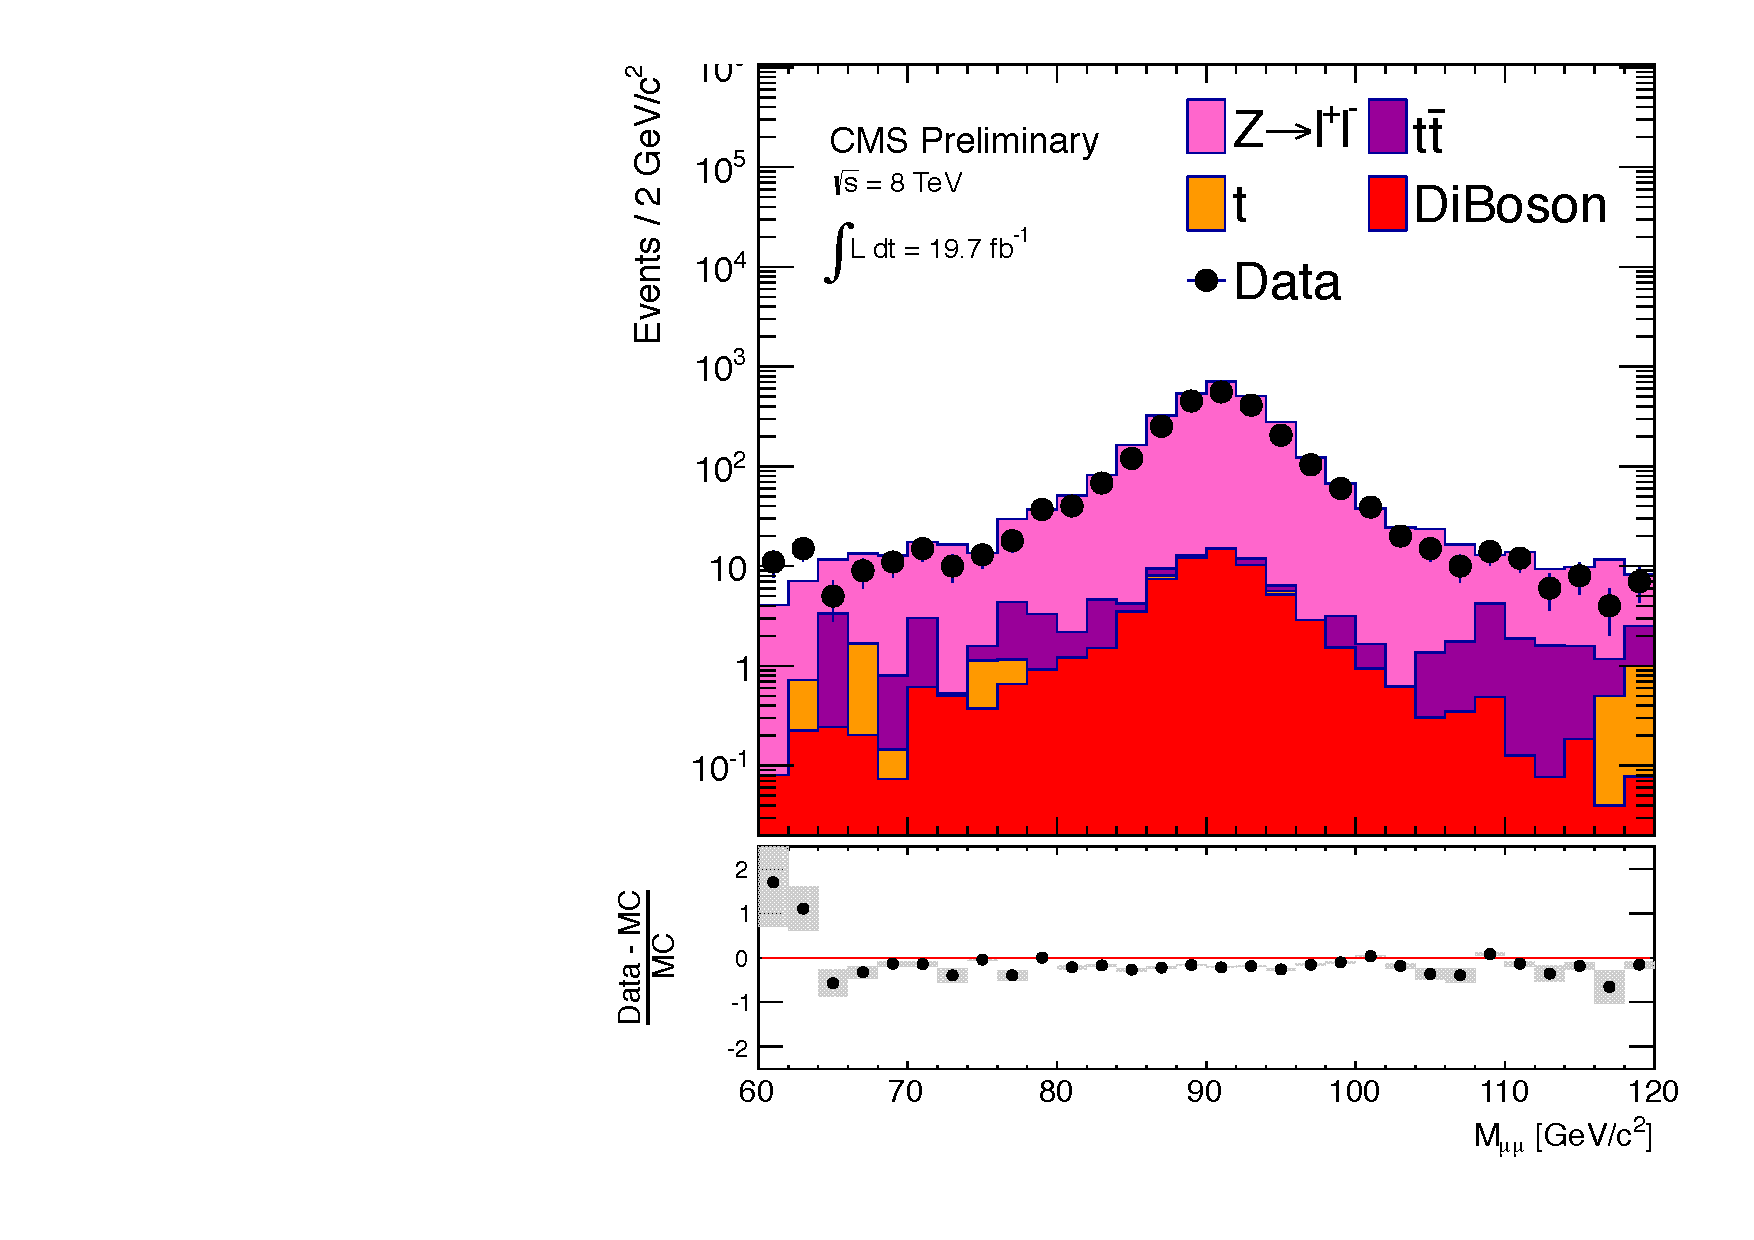
\includegraphics[scale=0.39]{Figures/sus13009/cut/ZleplepMT_60_120_prelim.pdf}
  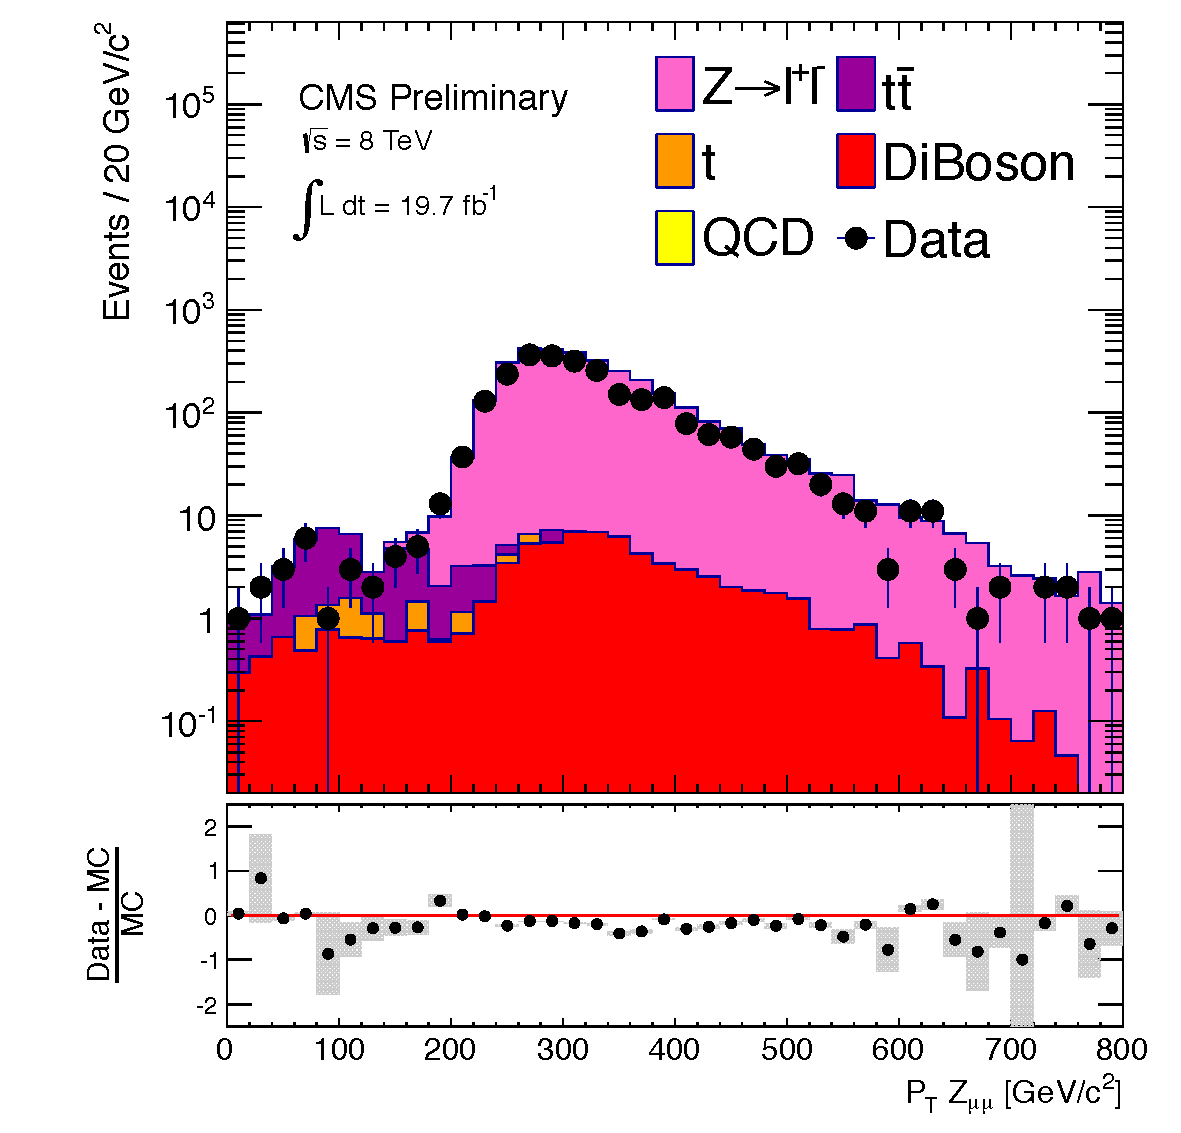
\includegraphics[scale=0.39]{Figures/sus13009/cut/ZleplepPT_60_120_prelim.pdf}
  \caption{Invariant mass and transverse momentum of the dimuon pair in the \zmumu control sample.}
  \label{fig:BKGR_Z_mass}
  \end{center}
\end{figure}

The \zmumu and \znunu events share similar kinematic characteristics and by interpreting the pair of muons as missing energy, the topology of the process in which the $Z$ boson decays to neutrinos can be reproduced.  
A comparison between data and MC for the dimuon invariant mass and momentum after all the selection cuts and requiring $\pt(\jet_1)>250~\GeV$ is shown in Figure~\ref{fig:BKGR_Z_mass}.
The number of \znunu events can then be predicted using:

\begin{equation}
N(Z\rightarrow\nu\nu) = \frac{N^{\rm obs}_{\mu\mu} - N^{\rm bgd}_{\mu\mu}}{A*\epsilon}\cdot R ,
\label{eq:znunudatadriven}
\end{equation}
where $N^{\rm obs}_{\mu\mu}$ is the number of observed dimuon events, $N^{\rm bgd}_{\mu\mu}$ is the number of non-\zmumubr{} events contributing to the dimuon sample, $A$ is the acceptance of the control sample criteria and $\epsilon$ is the selection efficiency of a reconstructed event provided it was produced within the acceptance of the criteria, and $R$ is the ratio of branching fractions for the $Z$ decay to neutrinos and a pair of muons. These factors are determined as follows:
\begin{itemize}

\item $ N^{\rm bgd}_{\mu\mu}$ : The dimuon sample comprises predominantly of \zmumu{} events with contamination from other, non-\zmumubr{} processes at the level of 5\%. These backgrounds are taken from simulation and a relative 50\% uncertainty is assigned their yields; 

\item $A$ : The acceptance $A$ is defined as the fraction of all generated events, prior to hadronization and reconstruction 
(i.e. at quark and lepton level as described by the event generator), that satisfy the requirements of the control sample. 
One muon must satisfy $\pt > 20$~\GeV{} and $|\eta| < 2.1$, and the other, of opposite sign, must satisfy $\pt > 10$~\GeV{}. The invariant mass of these muons must lie within 60 \GeV{} and 120~\GeV{}. This is obtained from $\Z${}\,+\,jets simulation;

\item $\epsilon$ : The event selection efficiency $\epsilon$ is defined as the efficiency of reconstructing two muons passing all the identification and isolation criteria that have a reconstructed invariant mass between 60 and 120 $\GeV$, given that they are within the detector acceptance $A$. 
The efficiency is taken from simulation, once it has passed through the hadronization and reconstruction stages (unlike for $A$).
%
The efficiency of reconstructing a \zmumubr{} event with two tight muons is calculated in both data and simulation (for all MC simulated samples) in the \zmumu{} control sample. The difference in efficiencies is averaged across the search region jet \pt{} thresholds, and the resulting correction factor of 1.005 is applied to $\epsilon$ to account for the difference in muon selection efficiency between data and MC;

\item $R$ : The ratio of the branching fraction $R = (\frac{BF(\znunubr)}{BF(\zellellbr)})$ is obtained from Ref.~\cite{PDG} and 
   is $5.942\pm 0.019$ when $l=\mu$. 
\end{itemize}
 
The prediction of the \znunubr{}\,+\,jets background in the search regions relies on counting the number of 
\zmumubr{}\,+\,jets events at each $\pt(\,\mathrm{j}_1)$ threshold, which is in turn
correlated to the \METmu requirement.
In the definition of \METmu, we interpret muons as missing energy: 
muon \ptv is added into the \METv to calculate \METvmu.
As the \METvmu in an event is largely balanced by $\ptv(\,\mathrm{j}_1)$, 
the values of \METmu and $\pt(\,\mathrm{j}_1)$ thus rely on successfully 
identifying both muons arising from a \zmumu decay. 

If either (or both) of the muons in a \zmumu decay is not properly identified, 
then the value of \METmu may be wrong.
For example, if one of the muons does not pass identification requirements but the track is reconstructed, 
then the energy of that muon will be included within the \METv calculation (reconstructed using the \ac{PF} algorithm).
However, the muon will not be identified using tight or loose requirements, and its \ptv will not be included in the \METvmu calculation.
The value of \METvmu will then be incorrect, 
and the event is likely to fail the selection requirements on \METmu or $\pt(\,\mathrm{j}_1)$.
%
It will not contribute to the total number of \zmumubr{}\,+\,jets events and therefore reduce the total \znunubr{}\,+\,jets background estimation.
However, if it had of been a \znunubr{}\,+\,jets event, 
both neutrinos would lead to \MET --- in neglecting such events we underestimate the \znunubr{}\,+\,jets background.


\begin{figure}%[!Hhtb]
  \begin{center}
  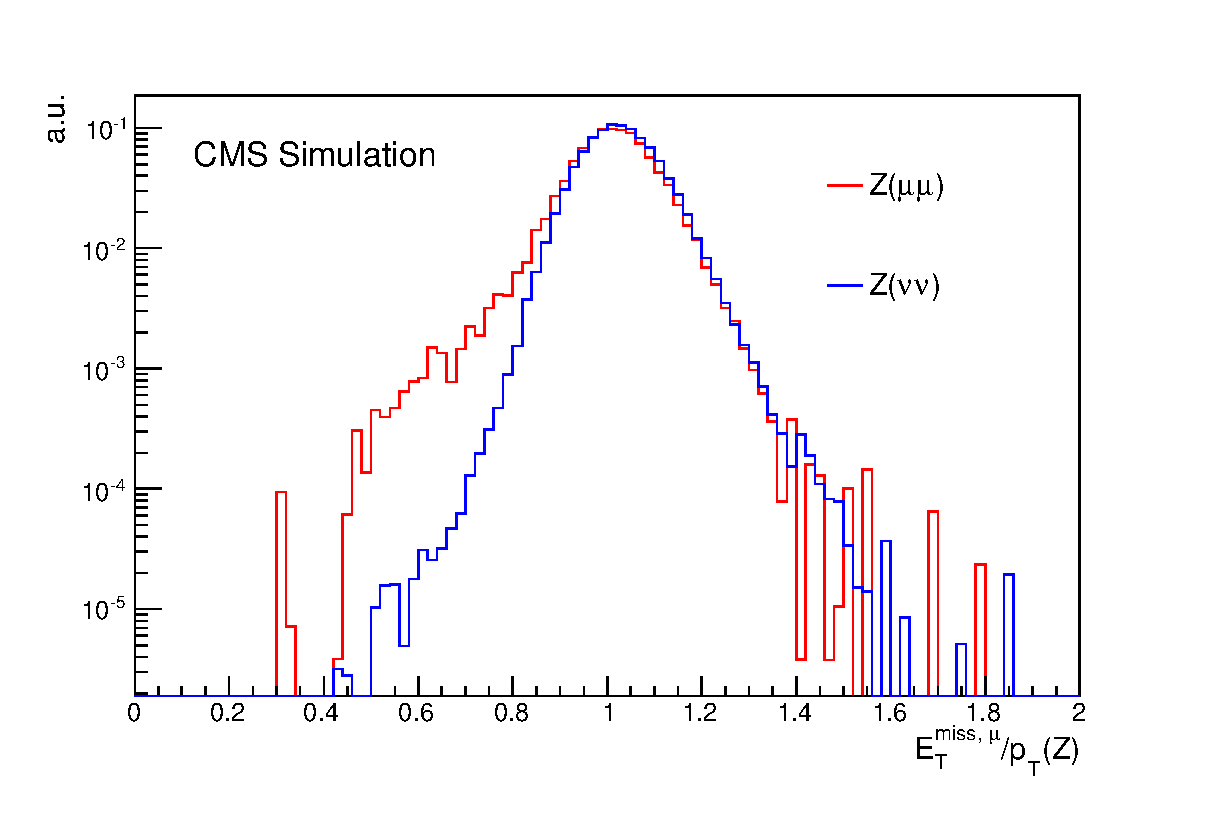
\includegraphics[scale=0.55]     {Figures/sus13009/ratioMETnoMu_GenZpT.eps}
   \caption{The ratio of \METmu to the \Z{} boson \pt, taken from simulation, in \zmumubr{}\,+\,jets and \znunubr{}\,+\,jets events. Distributions are normalized to unit area.
         \label{fig:metratio}}
  \end{center}
\end{figure}

Figure~\ref{fig:metratio} shows the distribution of the ratio of \METmu to the \pt{} of the \Z{} boson $\pt(\Z)$, 
taken from \zmumubr{}\,+\,jets and \znunubr{}\,+\,jets simulation. 
The larger tail at low values of $\METmu/\pt(\Z)$ in \zmumubr{}\,+\,jets events is attributed to events where one or both muons is not properly identified as described above.
In order to correct for this effect we count the number of events in simulation where the ratio $\METmu/\pt(\Z)< 0.7$, at each $\pt(\,\mathrm{j}_1)$ threshold in the dimuon control sample, with the additional criteria that the $\pt(\Z{})>250$~\GeV{} to ensure $\METmu$, when measured correctly, $>250~\GeV$. 
The value of 0.7 is chosen because the resolution of the \Z{} boson mass peak is $\sim 0.3$, and we wish to count events in the tail of the spectrum.
This gives an estimation of the number of events where we have not properly measured or identified one or two of the muons. 
The ratio in each search region is shown in Table~\ref{tab:Zinv_genZMETmu_SF}. 
This correction factor is combined with the difference in data and simulation for muon selection efficiency (1.005, described above), and applied to $\epsilon$ in each search region.

\begin{table*}%[!Hhtb]  %table 8   110811:05  
        \begin{center}
\caption{Summary of the \zmumu event yields and the efficiency factors used to predict the \znunu\,+\,jets background.}
\label{tab:Zinv_genZMETmu_SF}
       \begin{tabular}{l|ccccccc} \hline
%& & & & \MET\ cut&  & &  \\
$\pt(\,\mathrm{j}_1)$ (\GeV) & $>$ 250 & $>$ 300 & $>$ 350 & $>$ 400& $>$ 450  & $>$ 500 & $>$ 550 \\ \hline 
$\METmu/\pt(\Z)< 0.7$ & 0.037 &  0.046 &  0.060 &  0.063 &  0.083  & 0.097 &  0.098 \\
\hline
       \end{tabular}   
                                                                                   
\end{center}
\end{table*}


%In addition, a 4.7$\%$ correction is applied to the predicted \znunu background to account for an inefficiency in \zmumu\ events where the muon track is reconstructed but the muon is not identified. These events were studied by plotting the ratio of \MET and the generated $Z$ boson \pt, they are present in the low tail of the distribution, below around 0.7, in \zmumu\ events but absent in the same distribution for \znunu events. 
%We therefore estimate the selection efficiency using Z\,+\,jets MC and assign a systematic of 2$\%$ to cover the variation of the data-MC scale factor from 1.0, measured in~\cite{bib:AN-11-240}.

A correction factor is applied to R in order to account for contamination from $\gamma^{*}$ events in the data that fall within the selection criteria of the control sample, as well as efficiency of the mass window requirement. 
Using \zmumubr{}\,+\,jets and \znunubr{}\,+\,jets simulated events, 
the $\gamma^{*}$ contamination $R^{\gamma^{*}}$ can be estimated using
   \begin{equation}
   R^{\gamma^{*}} = \frac{1-\alpha}{1-\beta} ,
   \end{equation}
where $\alpha$ is the difference in the normalized yield of \zmumubr{}\,+\,jets and \znunubr{}\,+\,jets events in the Z mass window, $60< m_{\Z{}} < 120~\GeV$, and
   $\beta$ is the fraction of events lying outside the Z mass window in \znunubr{}\,+\,jets simulation.
Normalized across all $\pt(\,\mathrm{j}_1)$ bins, we find a correction factor of 1.017.


Table~\ref{tab:Zinv_factors} shows the observed dimuon event yields, non-\zmumubr event yields, the acceptance $A$ and efficiency $\epsilon$. The ratio of branching fractions $R$ is corrected by $R^{\gamma^{*}}$, and given (it is the same for each threshold). 
The uncertainties on these factors are discussed below. 

%A summary of the fractional contributions of the uncertainties to the total error on the \znunu background is shown in Table~\ref{tab:Z_jets_sys}. 
%The dominant contribution to the uncertainty is the statistical uncertainty from the size of the \zmumu sample. 

%For the baseline selection, this is found to be 14131.5$\pm$xxxxx. This can be compared to the prediction from the invisible Z MC, 14728.9$\pm$xxxx.

\newsavebox{\cutflowBoxc}
\begin{table*}%[!Hhtb]  %table 8   110811:05  
        \begin{center}
\caption{Observed yields in the dimuon control sample, background yields from non-\zmumubr{} processes, $A$ and $\epsilon$ of control sample requirements and the corrected ratio of branching fractions in each of the search regions. }
%The data-driven \znunubr{}\,+\,jets background prediction is given in the final row.}
\label{tab:Zinv_factors}
         \begin{lrbox}{\cutflowBoxc}
       \begin{tabular}{l|ccccccc} \hline
$\pt(\,\mathrm{j}_1)$ (\GeV) & $>$ 250 & $>$ 300 & $>$ 350 & $>$ 400& $>$ 450  & $>$ 500 & $>$ 550 \\ \hline 
 $N^{\rm obs}_{\mu\mu}$ & 2547 &  1235 &  567&  277 & 150 & 79  & 40  \\ 
 $N^{\rm bgd}_{\mu\mu}$ & 111  &  64   &  35 &  19  & 8.9 & 4.4 & 2.7 \\ 
Acceptance $A$        & 0.805  & 0.833  & 0.851  & 0.864  & 0.881  & 0.905  & 0.896  \\
Efficiency $\epsilon$ & 0.862  & 0.843  & 0.822  & 0.802  & 0.775  & 0.751  & 0.754  \\
%R &         5.942 & 5.942 & 5.942 & 5.942 & 5.942 & 5.942 & 5.942  \\ 
$R$ & 6.043 & 6.043 & 6.043 & 6.043 & 6.043 & 6.043 & 6.043\\ 
\hline
%\znunu &21209$\pm$1115  &10077$\pm$592 &  4597$\pm$324 & 2250$\pm$197 & 1250$\pm$137 & 663$\pm$94 & 334$\pm$65 \\ 
%\znunu & 21209  & 10077 &  4597 & 2250 & 1250 & 663 & 334 \\ 

       \end{tabular}    
                \end{lrbox}
\scalebox{0.99}{\usebox{\cutflowBoxc}}
\end{center}
\end{table*}

\subsubsection{Uncertainties on data-driven \znunubr{}\,+\,jets background estimation}

The dominant source of uncertainty on the \znunubr{}\,+\,jets background estimation arises from statistical uncertainties on $N^{\rm obs}_{\mu\mu}$.
It increases as the $\pt(\,\mathrm{j}_1)$ threshold is increased, and contributes 2.1--17\%.

The uncertainty on $N^{\rm bgd}_{\mu\mu}$, arising from non-\zmumubr processes, is taken as 
50\% of the respective yields, where the total uncertainty on $N^{\rm bgd}_{\mu\mu}$ is the quadratic sum of the individual contributions. 
As the total contribution from non-\zmumubr processes in the control region is small, of order 5\%, this uncertainty has a relatively minor contribution to the total uncertainty, varying from 1.6--3.5\%.

The total uncertainty on $A$ arises from both statistical and systematic sources. 
The statistical uncertainty is due the number of simulated events used to derive the ratio. 
A 2\% systematic uncertainty is added to this, to incorporate the uncertainty on the \ac{PDFs} used to describe the colliding protons.
Similarly, the total uncertainty on $\epsilon$ is due to the statistics of the simulation and incorporates a 2\% systematic uncertainty on the hadronization process. 
These systematics dominate over the statistical uncertainties, where the total uncertainty on $A$ varies from 2.0--2.9\%, and on $\epsilon$ from 2.1--5.5\%. 
There are fewer events with muons reconstructed within the kinematic acceptance of the control sample than are generated within the kinematic acceptance, hence the statistical uncertainty - and therefore total uncertainty - on $\epsilon$ is larger than the uncertainty on $A$.

A 2\% systematic uncertainty is assigned to $R$, in order to incorporate the uncertainties on the 
ratio of branching fractions (which are much smaller than 2\%), 
and on the correction factor $R^{\gamma^{*}}$ (itself less than 2\%), which incorporates 
the uncertainty due to the restriction of the Z mass window on branching fractions,
and on the contribution of $\gamma^{*}$ events in the control sample.

The uncertainties from the various sources are added in quadrature, and are listed in Table~\ref{tab:Z_jets_sys}. 
The total uncertainty varies between 5.3 and 19\%. 

\begin{table*}%[!Hhtb]  %table 8   110811:05  
        \begin{center}
\caption{Summary of the contributions to the total uncertainty on \znunu\,+\,jets background from the various factors used in the data-driven estimation.}
\label{tab:Z_jets_sys}
                \begin{tabular}{l|ccccccc} \hline
$\pt(\,\mathrm{j}_1)$ (\GeV) & $>$ 250 & $>$ 300 & $>$ 350 & $>$ 400& $>$ 450  & $>$ 500 & $>$ 550 \\ \hline 
Statistics ($N^{\rm obs}_{\mu\mu}$)  & 2.1 &  3.0 &  4.5 &  6.5 &  8.7 &  12  &  17 \\
Background ($N^{\rm bgd}_{\mu\mu}$)  & 1.6 &  2.0 &  2.4 &  2.7 &  2.9 &  2.9 &  3.5\\ 
Acceptance              & 2.0 &  2.1 &  2.1 &  2.2 &  2.4 &  2.5 &  2.9\\
Efficiency              & 2.1 &  2.1 &  2.3 &  2.6 &  3.3 &  4.4 &  5.5\\
R                       & 2.0 &  2.0 &  2.0 &  2.0 &  2.0 &  2.0 &  2.0\\ \hline
Total                   & 5.3 &  5.9 &  7.0 &  8.8 &  11  &  14  &  19 \\  \hline 
\end{tabular}
\end{center}
\end{table*}

The final data-driven evaluation of the \znunubr{}\,+\,jets background using the methods outlined above is shown in Table~\ref{tab:finalznunu}.

\newsavebox{\cutflowBoxd}
\begin{table*}%[!Hhtb]  %table 8   110811:05  
        \begin{center}
\caption{Observed yields in the dimuon control sample, background yields from non-\zmumubr{} processes, $A$ and $\epsilon$ of control sample requirements and the corrected ratio of branching fractions in each of the search regions. }
%The data-driven \znunubr{}\,+\,jets background prediction is given in the final row.}
\label{tab:finalznunu}
         \begin{lrbox}{\cutflowBoxd}
       \begin{tabular}{l|ccccccc} \hline
$\pt(\,\mathrm{j}_1)$ (\GeV) & $>$ 250 & $>$ 300 & $>$ 350 & $>$ 400& $>$ 450  & $>$ 500 & $>$ 550 \\ \hline 
\znunubr{}\,+\,jets &21209$\pm$1115  &10077$\pm$592 &  4597$\pm$324 & 2250$\pm$197 & 1250$\pm$137 & 663$\pm$94 & 334$\pm$65 \\ 
\hline
       \end{tabular}    
                \end{lrbox}
  \scalebox{0.87}{\usebox{\cutflowBoxd}}
\end{center}
\end{table*}
%//////////////////////////////////////////////////////////////////////////////////////////

\subsection{Data-driven \wlnubr{}\,+\,jets background estimation}
\label{sec:wjets}

The second largest contribution to the total SM background arises from \wlnubr{}\,+\,jets events. 
The lepton (\e and \mu, including those from leptonically decaying $\tau$ leptons) fails the respective lepton veto
and hence is ``lost'', i.e. it is not isolated, not identified, or outside of the acceptance of 
the analysis. 
Similarly, \tauh leptons which are not identified contribute to this lost-lepton background.
The contributions in the search regions from lost-lepton events are evaluated in a similar way to the \znunubr{}\,+\,jets background, using a muon control sample enriched in \wmunubr{}\,+\,jets events.

From the muon control sample defined using the same triggers as the search regions with the exception of the muon veto, a sample enriched in \wmunubr{}\,+\,jets events is obtained by requiring one muon satisfying the tight muon criteria with a reconstructed \W{}-boson transverse mass $m_{T} = \sqrt{2 \pt^{mu} \met (1 - \cos{\Delta \phi}) }$ that lies between 50 and 100~GeV, where $\Delta\phi$ is the azimuthal angle between the \metvmu and $\ptv^{\mu}$ vectors.
Event yields in the \wmunubr{}\,+\,jets-enriched single muon control sample are listed in Table~\ref{tab:Wmuontable} with the predicted SM processes from simulation. 
A comparison between data and MC for the transverse mass and momentum of the \W{} boson after the full selection and for $\pt(\,\mathrm{j}_1) > 250~\GeV$ is shown in Figure~\ref{fig:BKGR_W_mass}.

\begin{table*}[!Hhtb]
        \begin{center}
\caption{Event yields for the $W \rightarrow \mu \nu$ data control sample with SM backgrounds from MC simulation.
A relative uncertainty of 50\% is assigned to each background (i.e. from $\Z$\,+\,jets, \ttbar, single top, QCD and diboson events) and these are combined in quadrature to get the total uncertainty 
on the number of background events in the $W \rightarrow \mu \nu$ sample.}
\label{tab:Wmuontable}
 {\small
  \begin{tabular}{l|ccccccc} \hline
%numbers 1July
$\pt(\,\mathrm{j}_1)$ (\GeV) & $>$ 250 & $>$ 300 & $>$ 350 & $>$ 400& $>$ 450  & $>$ 500 & $>$ 550 \\ \hline 
\wpj                & 11436 & 5712  & 2694 & 1349 & 712  & 389  & 223  \\
\zellellbr{}\,+\,jets & 183   & 94    & 44   & 22   & 9.9  & 6.6  & 3.7  \\
\znunubr{}\,+\,jets   & 0     & 0     & 0    & 0    & 0    & 0    & 0    \\
\ttbar              & 608   & 313   & 151  & 76   & 41   & 20   & 11   \\
Single top quarks   & 158   &  80   & 41   & 22   & 13   & 7.8  & 4.8  \\
QCD multijet        & 0.3   & 0.3   & 0.3  & 0.3  & 0.3  & 0.3  & 0.3  \\
Diboson             & 197   & 121   & 71   & 41   & 22   & 13   & 6.5  \\
\hline
Total MC            & 12582  & 6320  & 3001  & 1509  & 798  & 437  & 249  \\
Data                & 11371  & 5477  & 2547  & 1258  & 668  & 352  & 184  \\
\hline
                \end{tabular}}                                                              
                \end{center}
\end{table*}



\begin{figure}[!Hhtb]
  \begin{center}
  %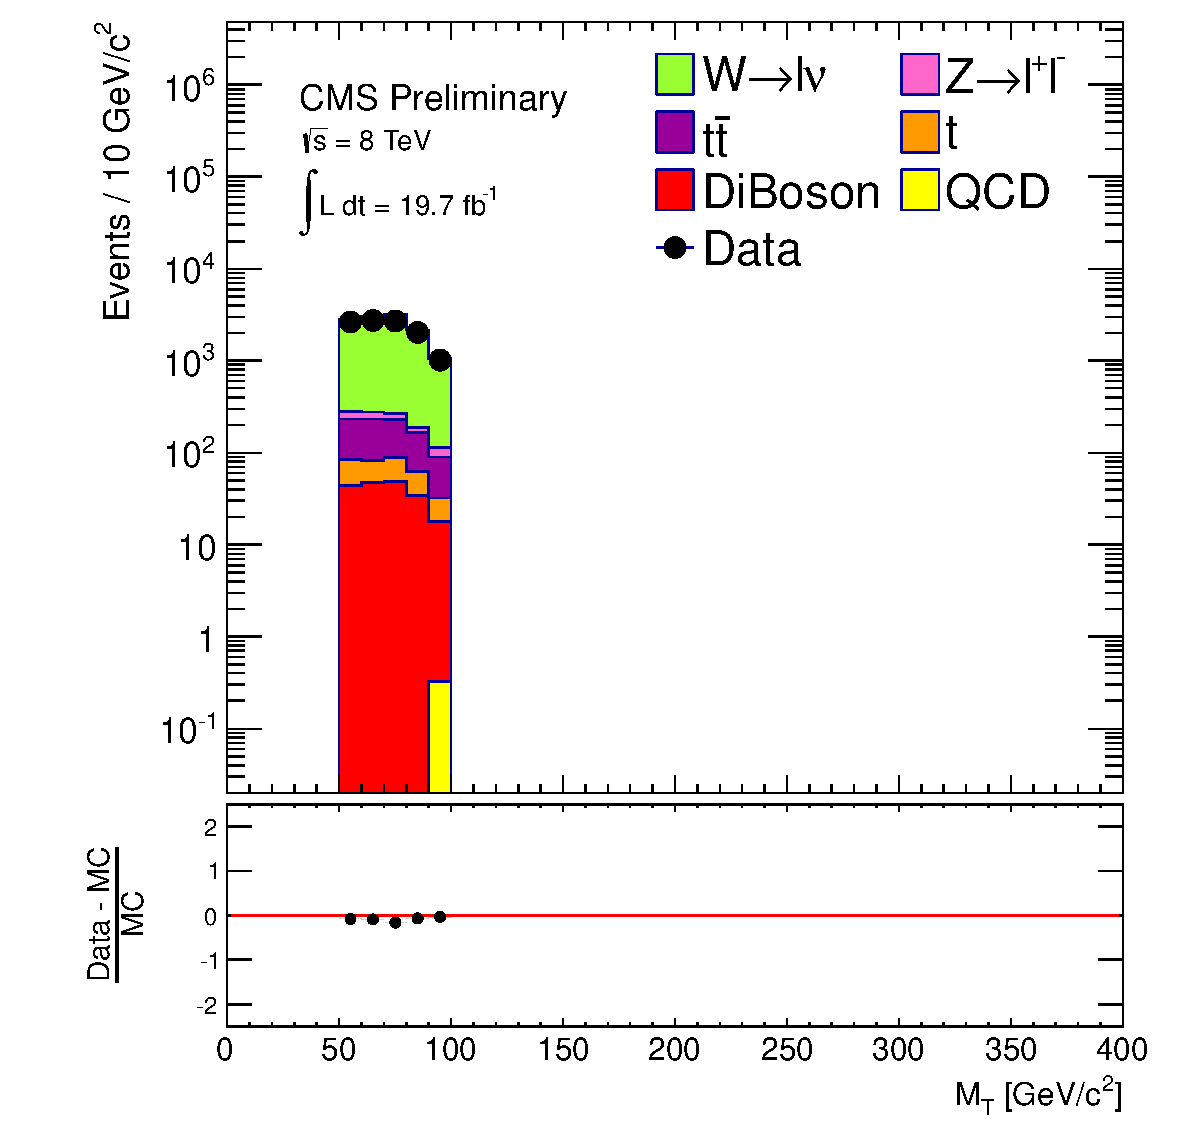
\includegraphics[scale=0.39]{cut/WlepnuMT_50_100.pdf}
  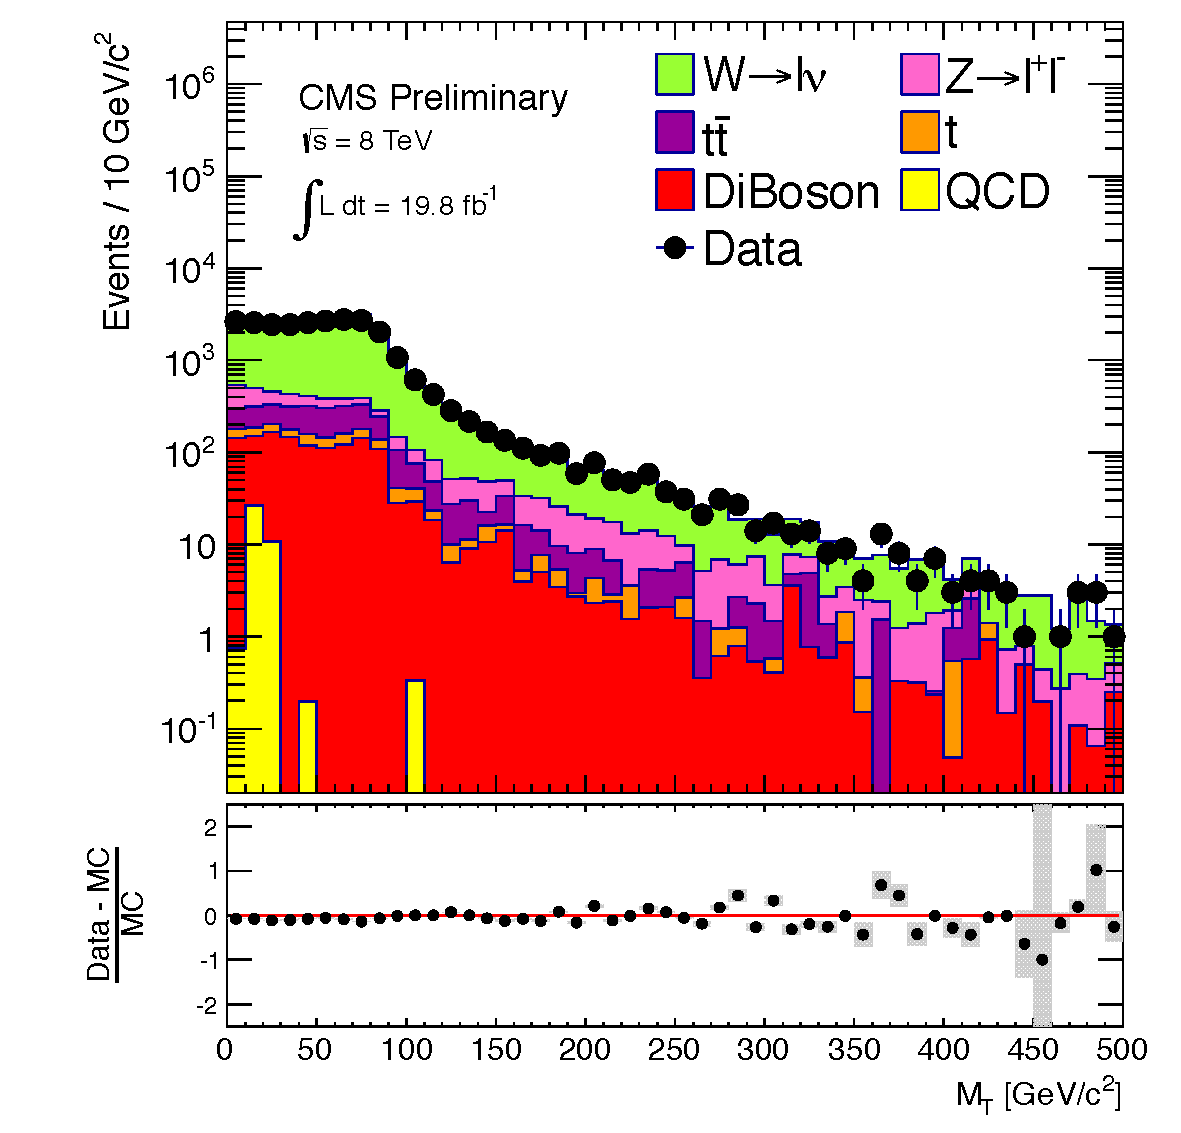
\includegraphics[scale=0.39]{Figures/sus13009/cut/WlepnuMT_prelim.pdf}
  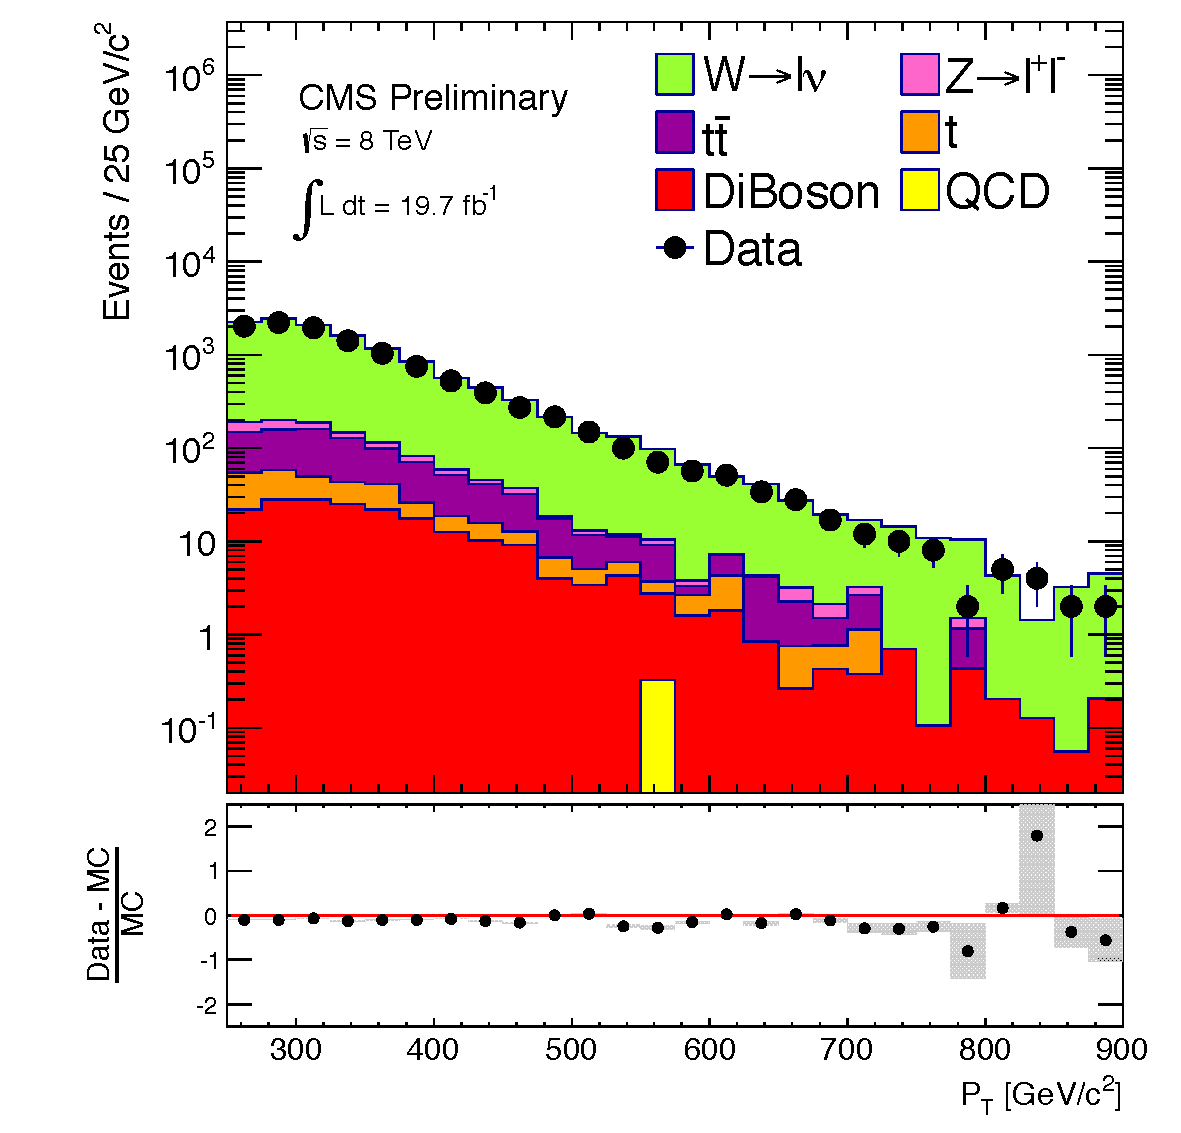
\includegraphics[scale=0.39]{Figures/sus13009/cut/WlepnuPT2_50_100_prelim.pdf}
  \caption{Transverse mass $m_{T}$ of the muon (left) and \pt{} of $W^\pm$ candidates in the W mass window, $50 - 100~\GeV$ in the single muon control sample.}
  \label{fig:BKGR_W_mass}
  \end{center}
\end{figure}

The total number of \wmunubr{}\,+\,jets events is estimated in an analogous way to the \znunubr{}\,+\,jets background,
correcting the observed number of single muon events in the control sample $N^{\rm obs}_{\mu}$ by events due to non-\wpj{} processes $N^{\rm bgd}_{\mu}$.  
The resulting \wmunu events are then corrected for the kinematic acceptance $A'$ of the control sample, and the efficiency $\epsilon'$ of reconstructing events within the acceptance in the detector to obtain the total number of generated events ($N^{\rm tot}_{\mu}$):
\begin{equation}
N^{\rm tot}_{\mu} = \frac{N^{\rm obs}_{\mu} - N^{\rm bgd}_{\mu}}{A'\epsilon'}.\label{eqn:Ntot}
\end{equation}

The resulting number of \wmunu events produced in the detector is subsequently weighted by a muon veto inefficiency factor in order to obtain the predicted number of \wmunubr{}\,+\,jets events that would not be rejected by the lepton veto and thus remain in the search regions.
%
The total number of \wmunubr{}\,+\,jets events that are out of the acceptance and not identified or isolated can be written as:
\begin{equation}
N^{\rm lost}_{\mu} = N^{\rm tot}_{\mu}(1 - A_{\mu}\epsilon_{\mu}).
\end{equation}
%\begin{eqnarray}
%N_{!A}^{\mu} &=& N_{tot}^{\mu}*(1 - A_{\mu})\\
%N_{!\epsilon}^{\mu} &=& N_{tot}^{\mu}*A_{\mu}*(1 - \epsilon_{\mu})\\
%\end{eqnarray}
where $A_{\mu}$ is the acceptance of the loose muon selection requirements (used in the muon veto) before any reconstruction has taken place, 
and $\epsilon_{\mu}$ is the efficiency of the reconstruction for muons satisfying selection requirements when produced (i.e. for muons within the acceptance $A_{\mu}$).
$A_{\mu}$ and $\epsilon_{\mu}$ are estimated using simulation, and $\epsilon_{\mu}$ is corrected for differences in muon selection efficiency between data and MC in the same way as for $\epsilon$ in the \znunubr{}\,+\,jets background estimation.

To estimate the lost electron background, we begin by finding the total number of \wenu events produced $N^{\rm tot}_{\e}$.
The ratio of the number of \wmunubr{}\,+\,jets to \wenubr\,+\,jets events produced, before any reconstruction has taken place, is taken from simulation and labelled $f_{\e}$.  
Then, $N^{\rm tot}_{\e} = N^{\rm tot}_{\mu}  f_{\e}$. 
The number of lost \wenu events can subsequently be found by correcting for the electron veto inefficiency factor:
\begin{eqnarray}
N^{\rm lost}_{\e} &=& N^{\rm tot}_{\e}(1 - A_{\e}\epsilon_{\e}).
\end{eqnarray}
Both the $A_{\e}$ and $\epsilon_{\e}$ factors are obtained using simulation, where $A_{\e}$ is the acceptance of the loose electron selection requirements (used in the electron veto) before any reconstruction has taken place, 
and $\epsilon_{\e}$ is the efficiency of reconstruction for electrons satisfying selection requirements when produced (i.e. for electrons within the acceptance $A_{\e}$).
A data/MC scale factor of 1.0 is assumed. % with an assigned systematic that covers the variation in efficiency between data and MC.
%Table~\ref{tab:wjetslost} summarises the estimated lost muon and electron background.
%A detailed table showing the various factors that are used to estimate this background is shown in Table~\ref{tab:wjets-summary}.

%The same procedure as that outlined in the above equations is then followed to obtain the number of events where the electron is not reconstructed/isolated or out of the acceptance. The electron acceptance is obtained using generator level MC and the selection efficiency is also obtained from MC with an assigned systematic that covers the variation in efficiency between data and MC.
%~\cite{bib:AN-11-240}.
The component of the \wpj{} background from \tauh events is estimated in the same way. 
The ratio of the number of \wmunubr{}\,+\,jets to \wtauhnubr\,+\,jets events ($f_{\tau}$) produced prior to reconstruction is taken from simulation and used to obtain $N^{\rm tot}_{\tau}$. This is subsequently weighted by the inefficiency of the tau selection used in the $\tauh$ veto to obtain the lost-lepton background due to \tauh events:
\begin{eqnarray}
N^{\rm tot}_{\tauh}  &=& N^{\rm tot}_{\mu}f_{\tauh},\\
N^{\rm lost}_{\tauh} &=& N^{\rm tot}_{\tauh}(1 - A_{\tauh}\epsilon_{\tauh}).
\end{eqnarray}
The \tauh identification acceptance and efficiency is estimated from simulation with a data/MC scale factor of 1.0 and assigned an uncertainty of 6$\%$ as recommended by the \ac{CMS} Tau Physics Object Group. 
The electron and muon discriminants in the tau identification can also result in the tau veto rejecting electron and muon events. 
The probability of an electron or muon to fake a tau is estimated from \wpj{} simulation and found to be negligible, below 0.1\%.
% No correction is made to these fake rates to account for data/MC differences as recommended by the Tau POG.  The Tau POG recommends an uncertainty of 5$\%$ on the electron fake rate for electrons in the Barrel and 10$\%$ for those in the Endcap and a 30$\%$ uncertainty on the muon fake rate. Since the fake rates are very small for our analysis, we assign 10$\%$ to electrons in both the Barrel and Endcap and the recommended 30$\%$ for muons. 
% Table~\ref{tab:wjetstau-summary} shows the tau acceptance and efficiency that are used to obtain the remaining tau hadronic background. More details on the tau acceptance, efficiency and fake rates at different stages of the monojet selection are given in Table~\ref{tab:wjets-hadronictau}. 

All of the above components can be summarised in a `master' equation for estimating the lost-lepton background:
\begin{equation}
N^{\rm lost}_{lep} = \frac{N^{\rm obs}_{\mu} - N^{\rm bgd}_{\mu}}{A'\epsilon'}\Big[(1 - A_{\mu}\epsilon_{\mu}) + f_{\e}(1 - A_{\e}\epsilon_{\e}) + f_{\tauh}(1 - A_{\tauh}\epsilon_{\tauh})\Big]
\label{eq:lostleptotal}
\end{equation}
The factors in Eq.~\ref{eq:lostleptotal} used to estimate the lost muon, electron and hadronic tau backgrounds are listed in Table~\ref{tab:wjetslost}. 


\newsavebox{\cutflowBoxe}
\begin{table*}%[!Hhtb]  %table 8   110811:05  

        \begin{center}
\caption{Estimation of the remaining \wpj{} background from the lost electron, muon and hadronic tau contributions.}
\label{tab:wjetslost}
         \begin{lrbox}{\cutflowBoxe}
 \begin{tabular}{l|ccccccc} \hline
% & & & Met cut&  & & & \\
$\pt(\,\mathrm{j}_1)$ (\GeV) & $>$250 &$>$300 & $>$350 & $>$400& $>$450  & $>$500 & $>$550 \\ \hline 
$N^{\rm obs}_{\mu}$  & 11371 &  5477 & 2547 & 1258 & 668 &  352 &  184 \\
$N^{\rm bgd}_{\mu}$  & 1146  &  608  & 307  & 160  & 86  &  48  &  26  \\
$A'\epsilon'$   & 0.345 &  0.345 &  0.341 & 0.346 &  0.349 &  0.361 &  0.371 \\
$N^{\rm tot}_{\mu}$ & 29666 &  14125 &  6573  & 3176  &  1666  &  841   &  425   \\ \hline
 % 
{\bf Lost \mu} & & & & & & & \\
$A_{\mu}\epsilon_{\mu}$ & 0.887 &   0.895 &   0.901 &   0.908 &   0.908&    0.906 &   0.907  \\
$N^{\rm lost}_{\mu}$          & 3350  &   1484  &   649   &   292   &   152  &    79    &   40     \\ \hline
%
{\bf Lost \e} & & & & & & & \\
$A_{\e}\epsilon_{\e}$ &0.615 &  0.684 &  0.734 &  0.771 &  0.793 &  0.815 &  0.823\\
$f_{\e}$                &0.374 &  0.465 &  0.548 &  0.610 &  0.653 &  0.706 &  0.727\\
$N^{\rm lost}_{\e}$     &4273  &  2077  &  958   &  444   &  225   &  110   &  55   \\ \hline
%
{\bf Lost \tauh}& & & & & & & \\
$A_{\tauh}\epsilon_{\tauh}$ & 0.253  & 0.284  & 0.298  & 0.296  & 0.294  & 0.341  & 0.325 \\
$f_{\tauh}$                   & 0.212  & 0.235  & 0.235  & 0.228  & 0.212  & 0.201  & 0.195 \\
$N^{\rm lost}_{\tauh}$     & 4704   & 2377   & 1083   & 510    & 249    & 112    & 56    \\ 
\hline
%N$_{lost}$ & 12328$\pm$707 &  5939$\pm$366 & 2690$\pm$180 & 1246$\pm$92 &  627$\pm$52 & 301$\pm$29 & 150$\pm$18 \\ \hline

       \end{tabular}
                       \end{lrbox}
  \scalebox{0.9}{\usebox{\cutflowBoxe}}                                                                                   
\end{center}
\end{table*}

\subsubsection{Uncertainties on the data-driven lost-lepton background}

The fractional contributions to the total uncertainty on the lost-lepton background are shown in Table~\ref{tab:wjetssys}.
The statistical uncertainty on the number of events in the single muon control sample contributes 1.0--8.6\% to the total uncertainty on the lost-lepton background, becoming dominant as the jet threshold increases and the number of \wmunubr{}\,+\,jets events surviving the high leading jet \pt{} requirement decreases.  
The statistical precision could be increased by using \wenubr\,+\,jets events in addition to \wmunubr{}\,+\,jets events, 
however this would require an additional electron-based trigger. 
The extra systematic uncertainties associated with combining the triggers mean there is little to be gained by doing this in this analysis.

The uncertainty on the non-\wpj{} processes in the single muon control sample contributes 3.3--4.4\% to the total uncertainty. 
It is taken to be 50\% of each individual contribution added quadratically, in the same way as for the \znunubr{}\,+\,jets background estimation --- here there is a larger yield from background processes, hence this uncertainty is larger than the similar numbers in Table~\ref{tab:Z_jets_sys}.

Systematic uncertainties due to hadronization, 2\%, (PDF, 2\%) uncertainties are absorbed into the uncertainties on $A'$, $A_{\e}$ and $A_{\tauh}$ ($\epsilon'$, $\epsilon_{\e}$ and $\epsilon_{\tauh}$).
No factor is added into $A_{\mu}$ and $\epsilon_{\mu}$ to avoid double-counting --- these 
uncertainties, related to the generation and reconstruction of simulated muon events, have already been considered in the calculation of $N^{\rm tot}_{\mu}$. 
They are reconsidered in the case of the lost electron and \tauh lepton events in order to account for any differences in their generation as compared to muon events.
The uncertainties on acceptance and efficiency in each calculation are considered fully correlated, 
because efficiency is dependent on acceptance and we wish to be conservative.
The uncertainties on data/MC scale factors and on the number of simulated events in the control samples are also considered.
The combined uncertainties on acceptances and efficiencies in the lost-lepton background estimation dominate the total uncertainty, contributing 4.5--7.1\%.


A summary of the lost-lepton background in the search regions is shown in Table~\ref{tab:wjetstotal}.  


%The remaining component of the W\,+\,jets background which is not accounted for by this method is that from hadronically decaying tau. This is taken from W\,+\,jets MC and corrected by the data/MC scale factor obtained from \wmunu\ events.
%Since the control sample for this background estimation is obtained by relaxing the track isolation veto, we estimate the TIV efficiency from MC for all the \MET\ regions and apply this efficiency to obtain the final W\,+\,jets prediction. 


% The uncertainty on the W\,+\,jets estimation includes; the statistical uncertainty on the number of single-muon events in the data, a 50$\%$ uncertainty on the background events obtained from MC, an uncertainty on acceptance from PDFs (2\%) and MC statistics and an uncertainty on the selection efficiency $\epsilon$ from the variation in the data/MC scale factor and MC statistics. A summary of the fractional contributions of these uncertainties to the total error on the W\,+\,jets background is shown in Table~\ref{tab:wjetssys}. 
% It is dominated by statistical uncertainty on $N_{obs}$ and 50\% uncertainties assigned to $N_{bkg}$.
\newsavebox{\cutflowBoxf}
\begin{table*}
        \begin{center}
\caption{Summary of the fractional contributions (in \%) to the total uncertainty on the W\,+\,jets background from the various factors used to estimate it.}
\label{tab:wjetssys}
         \begin{lrbox}{\cutflowBoxf}
                \begin{tabular}{l|ccccccc} \hline
$\pt(\,\mathrm{j}_1)$ (\GeV)  & $>250$ &$>$300 & $>350$ & $>400$& $>450$ & $>500$ & $>550$ \\ \hline 
Statistics ($N^{\rm obs}_{\mu}$) & 1.0 & 1.5 & 2.3 & 3.2 & 4.4 & 6.2 & 8.6  \\  
Background ($N^{\rm bgd}_{\mu}$ ) & 3.3 & 3.7 & 4.0 & 4.2 & 4.2 & 4.3 & 4.4  \\ 
$A'$                   & 2.0 & 2.0 & 2.0 & 2.0 & 2.0 & 2.1 & 2.1  \\ 
$\epsilon'$            & 2.0 & 2.1 & 2.2 & 2.4 & 2.7 & 3.1 & 3.7  \\ 
$A_{\mu}$              & 0.1 & 0.1 & 0.2 & 0.2 & 0.3 & 0.4 & 0.5  \\ 
$\epsilon_{\mu}$       & 0.1 & 0.1 & 0.2 & 0.2 & 0.3 & 0.4 & 0.6  \\ 
$A_{e}$                & 0.7 & 0.9 & 1.0 & 1.1 & 1.2 & 1.3 & 1.3  \\ 
$\epsilon_{e}$         & 0.7 & 0.9 & 1.0 & 1.1 & 1.2 & 1.3 & 1.4  \\ 
$A_{\tau}$             & 0.2 & 0.2 & 0.2 & 0.2 & 0.2 & 0.3 & 0.3  \\ 
$\epsilon_{\tau}$      & 0.2 & 0.2 & 0.2 & 0.2 & 0.2 & 0.3 & 0.3  \\  
Total $A$ \& $\epsilon$'s& 4.5 & 4.7 & 4.9 & 5.2 & 5.5 & 6.1 & 7.1  \\  \hline
Total                  & 5.7 & 6.2 & 6.7 & 7.4 & 8.2 & 9.7 & 12   \\  \hline 
\end{tabular}   
  \end{lrbox}
  \scalebox{0.87}{\usebox{\cutflowBoxf}}          
\end{center}
\end{table*}

%A summary of the fractional contributions of these uncertainties to the total error on the W\,+\,jets background is shown in Table~\ref{tab:W_jets_sys}.

%\begin{table*}%[!Hhtb]  %table 8   110811:05  
%        \begin{center}
%\caption{Summary of the contributions to the total uncertainty on W\,+\,jets background from the various factors used in the data-driven estimation.}
%\label{tab:W_jets_sys}
%                \begin{tabular}{l|ccccccc} \hline
% & & & & \MET cut & & & \\
%Source of Uncertainty  & 250 &300 & 350 & 400& 450  & 500 & 550 \\ \hline 
%Source of Uncertainty                          & $\MET > 250$ &$\MET > 300$ &$\MET > 350$ &$\MET > 400$ &   $\MET > 450$ & $\MET > 500$ & $\MET > 550$ \\ \hline 
%Statistics (N$_{obs}$) & 0.9 & 1.4 & 2.0 & 4.1 & 5.7 & 7.8 \\
%Background (N$_{bgd}$) & 7.8 & 6.8 & 5.7 & 5.8 & 5.8 & 5.4 & 7.3 \\
%Acceptance (A') & 2.0& 2.0 & 2.0 & 2.1 & 2.1 & 2.2 &  2.3 \\
%Selection efficiency ($\epsilon'$) & 2.1 & 2.2 & 2.5 & 2.9 & 3.6 & 4.6 & 5.9 \\
%Total & 
%        \end{tabular}                                                                                   
%\end{center}
%\end{table*}


\newsavebox{\cutflowBoxg}
\begin{table*}[!Hhtb] 
        \begin{center}
\caption{Summary of the estimated total remaining W\,+\,jets background.}% and its comparison with the MC prediction.}
\label{tab:wjetstotal}
\begin{lrbox}{\cutflowBoxg}
 \begin{tabular}{l|ccccccc} \hline
% & & & Met cut&  & & & \\
$\pt(\,\mathrm{j}_1)$ (\GeV)  & $>250$ &$>$300 & $>350$ & $>400$& $>450$ & $>500$ & $>550$ \\ \hline
 $N^{\rm tot}_{\mu}$       & 29666  &  14125  &  6573  & 3176   &  1666  &  841   &  425   \\ 
 $N^{\rm lost}_{\mu}$      &  3350  &   1484  &   649  &  292   &   152  &   79   &   40   \\ 
 $N^{\rm lost}_{\e}$       &  4273  &   2077  &   958  &  444   &   225  &  110   &   55   \\ 
 $N^{\rm lost}_{\tauh}$    &  4704  &   2377  &  1083  &  510   &   249  &  112   &   56   \\ 
 Lost-lepton               & 12328$\pm$707 &  5939$\pm$366 & 2690$\pm$180 & 1246$\pm$92 &  627$\pm$52 & 301$\pm$29 & 150$\pm$18 \\ \hline
\end{tabular}
  \end{lrbox}
  \scalebox{0.87}{\usebox{\cutflowBoxg}} 
\end{center}
\end{table*}



\subsection{QCD Background Estimation}
\label{section:QCD}

The QCD multijet contribution in the search regions is expected to be small, $\approx 2\%$.
It is evaluated using simulation, with data/MC correction factors derived from data control regions enriched in multijet events.

The QCD control region is defined using the search region event selection, 
apart from those cuts that remove the majority of the QCD: $\Delta \phi(\jet_1, \jet_2)<2.5$ and $\njets < 3$.
The \pt{} requirement used to count jets is varied between 20 and 80~\GeV, as this parameter is sensitive to the number of multijet events satisfying the requirements of the search regions. 
We further require $\Delta \phi (\METmu, \jet_{2}) < 0.3$, as this sideband is highly populated with multijet events in which the \MET has been mismeasured. 
Such events have back-to-back jets where the mismeasured \METvmu vector is aligned with the second jet and is in the opposite hemisphere to the leading jet. 
Figure~\ref{dphi_METj2} shows a comparison of the data and MC for this control region, where the excess of QCD multijet events is evident at low  $\Delta \phi (\METmu,\jet_{2})$.


\begin{figure}[htbp!]
\begin{center}
 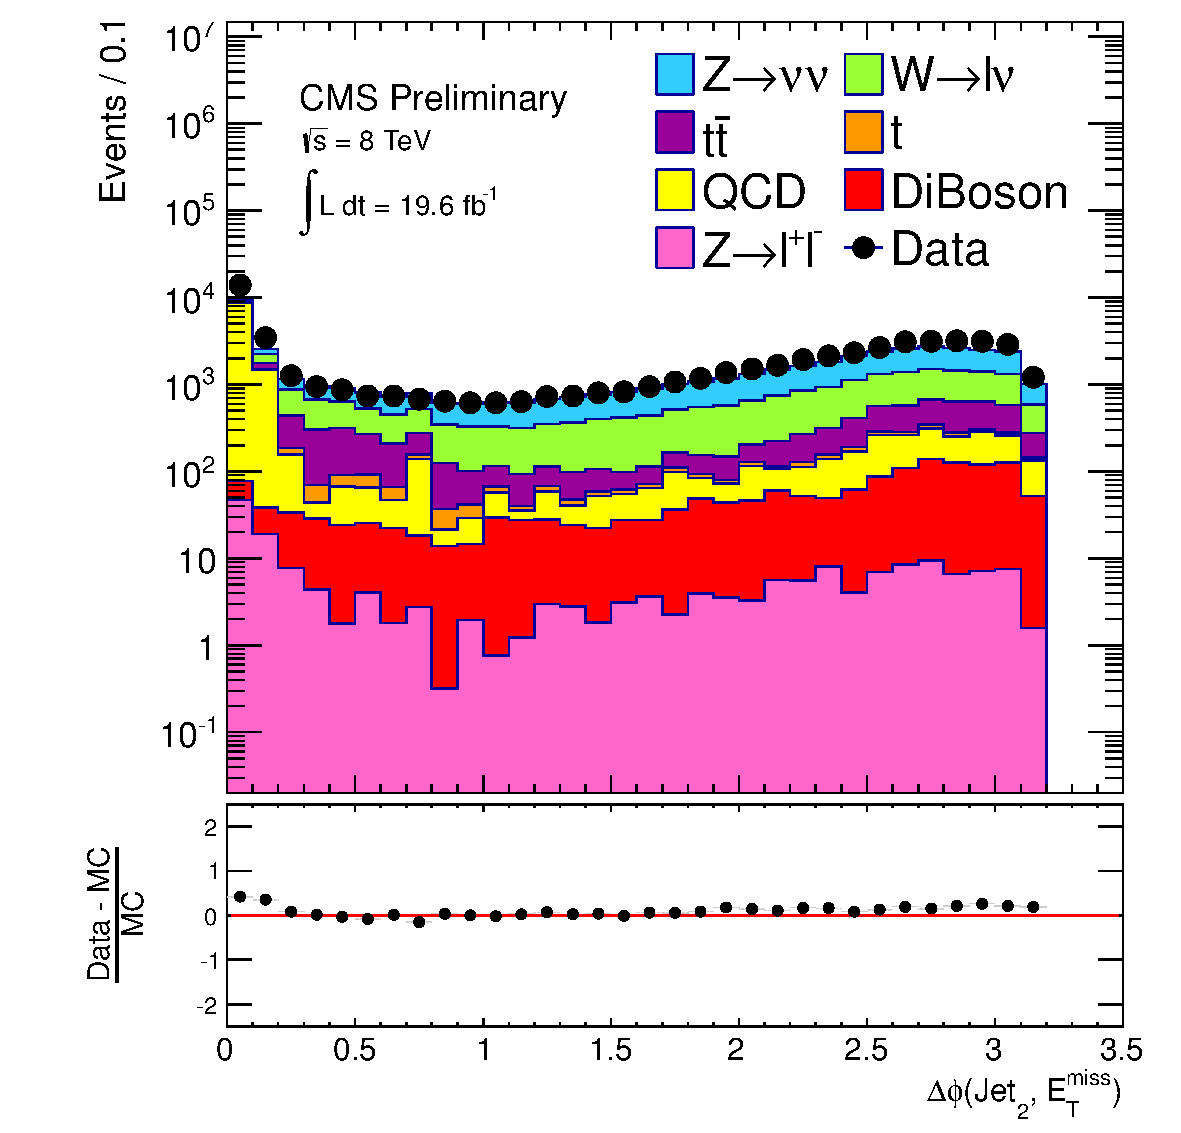
\includegraphics[scale=0.4]{Figures/sus13009/dPhi_MetLep_Jet2.pdf}
\caption{The QCD rich region dominated by back to back jets, $\Delta \phi(\METmu, \jet_2)<0.3$, shown for a jet counting cut of 60~\GeV{} for $\pt(\jet_1) > 250~\GeV$.}
\label{dphi_METj2}
\end{center}
\end{figure}


The event yields for data and MC in this region are shown in Table~\ref{QCDtable} for each jet counting \pt{} threshold and for $\pt(\jet_{1})>250~\GeV$. 
The scale factor $R^{\rm QCD}$ is defined as
\begin{equation}
\label{qcdSF}
R^{\rm QCD} = \frac{ N^{\rm obs}_{\rm QCD} - N^{\rm bgd}_{\rm QCD} }{ N^{\rm pred}_{\rm QCD} },
\end{equation}
where $N^{\rm obs}_{\rm QCD}$ is the observed number if events in the QCD control region and $N^{\rm bgd}_{\rm QCD}$ is the sum of the non-QCD events, taken from simulation and corrected with data/MC scale factors according to the data-driven estimations given in Section~\ref{sec:znunu} and \ref{sec:wjets} where applicable.


\begin{table}[htdp]
\caption{Event yields from MC and data for $\pt(\,\mathrm{j}_1)>250$~\GeV{} and for different values of the $\pt$ threshold used for jet counting in the QCD rich region $\Delta \phi (\MET, j_{2}) < 0.3 $. Relative uncertainty on a scale factor derived from the data is also shown.
}
\begin{center}
\begin{tabular}{c|cccc|cc} \hline
Jet \pt{} (\GeV)&  Data & Total Bkg  & QCD  & Total Data/MC &   $R^{\rm QCD}$ & Uncertainty\\ \hline
$>$ 20 & 21428 &  15987 &  10110& 1.340  & 1.538 & 0.321 \\ 
$>$ 30 & 20568 &  15141 &  10089& 1.358  & 1.538 & 0.325 \\
$>$ 40 & 19938 &  14543 &  10057& 1.371  & 1.536 & 0.329 \\
$>$ 50 & 19307 &  13974 &  9930 & 1.382  & 1.537 & 0.335 \\
$>$ 60 & 18708 &  13522 &  9852 & 1.384  & 1.526 & 0.341 \\
$>$ 70 & 18110 &  12921 &  9603 & 1.402  & 1.540 & 0.347 \\
$>$ 80 & 17435 &  12485 &  9455 & 1.397  & 1.523 & 0.354 \\ \hline 

\end{tabular}
\end{center}
\label{QCDtable}
\end{table}%


The QCD scale factor $R^{\rm QCD}$ in each search region is found by taking the mean scale factor from all the jet counting thresholds.
The scale factors applied to the QCD multijet event yield, from simulation, in search region are shown in Table~\ref{tab:QCDFinaltable}.
A correction factor of 1.53 at $\pt(\,\mathrm{j}_1) > 250~\GeV$ is required, decreasing to 1.35 at $\pt(\,\mathrm{j}_1) > 550~\GeV$. 
This is greater than the factor from the dijet resonance analysis of 1.22~\cite{CMS:exoDijetRes}, 
but the search regions here are in a different region of phase space so it is not unexpected.

\begin{table}[htdp]
\caption{QCD scale factor derived from QCD rich control region for each inclusive $\pt(\,\mathrm{j}_1)$ bin with relative error
}
\begin{center}
\begin{tabular}{c|cccccc} \hline
$\pt(\,\mathrm{j}_1)$ (\GeV) & QCD$_{s.f.}$ & Relative Error \\ \hline
250 &  1.534 &  0.336\\ 
300 &  1.490 &  0.336\\
350 &  1.465 &  0.341\\
400 &  1.428 &  0.350\\
450 &  1.402 &  0.359\\
500 &  1.365 &  0.369\\
550 &  1.347 &  0.377\\ \hline
\end{tabular}
\end{center}
\label{tab:QCDFinaltable}
\end{table}%


The total relative uncertainties on $R^{\rm QCD}$ are shown in Table~\ref{tab:QCDFinaltable}.
They are due to the statistical uncertainty on the number of events in data (which is negligible)
and the systematic uncertainty on the number of non-QCD events in the control regions. 
A relative uncertainty of 50\% is assigned to each non-QCD background, and contributions are added quadratically. 
To ensure we give a conservative estimation for the QCD multijet background, a relative uncertainty of 50\% is assigned to the yield taken from simulation, and this is combined in quadrature with the uncertainty on $R^{\rm QCD}$: total relative uncertainty on the multijet prediction is of order 60\%.  
The final QCD background estimation in the search regions is shown in Table~\ref{tab:QCDpred}.


\newsavebox{\cutflowBoxh}
\begin{table*}[!Hhtb] 
        \begin{center}
\caption{Summary of the estimated total remaining W\,+\,jets background.}% and its comparison with the MC prediction.}
\label{tab:QCDpred}
\begin{lrbox}{\cutflowBoxh}
 \begin{tabular}{l|ccccccc} \hline
% & & & Met cut&  & & & \\
$\pt(\,\mathrm{j}_1)$ (\GeV)  & $>250$ &$>$300 & $>350$ & $>400$& $>450$ & $>500$ & $>550$ \\ \hline
QCD     & 786$\pm$473 &  508$\pm$306 & 304$\pm$184 & 162$\pm$99 &  80$\pm$49 & 52$\pm$32 & 28$\pm$18 \\ \hline
\end{tabular}
  \end{lrbox}
  \scalebox{0.87}{\usebox{\cutflowBoxh}} 
\end{center}
\end{table*}



To provide a further cross check that the QCD prediction is sensible, we check the agreement for  $\Delta \phi (\MET, j_{3})$. 
Figure~\ref{dphi_METj3} shows the distribution for a jet counting threshold of 60~\GeV{} and $\pt(\,\mathrm{j}_1)>250$~\GeV; data agrees with MC within the assigned uncertainties.

\begin{figure}[htbp!]
\begin{center}
 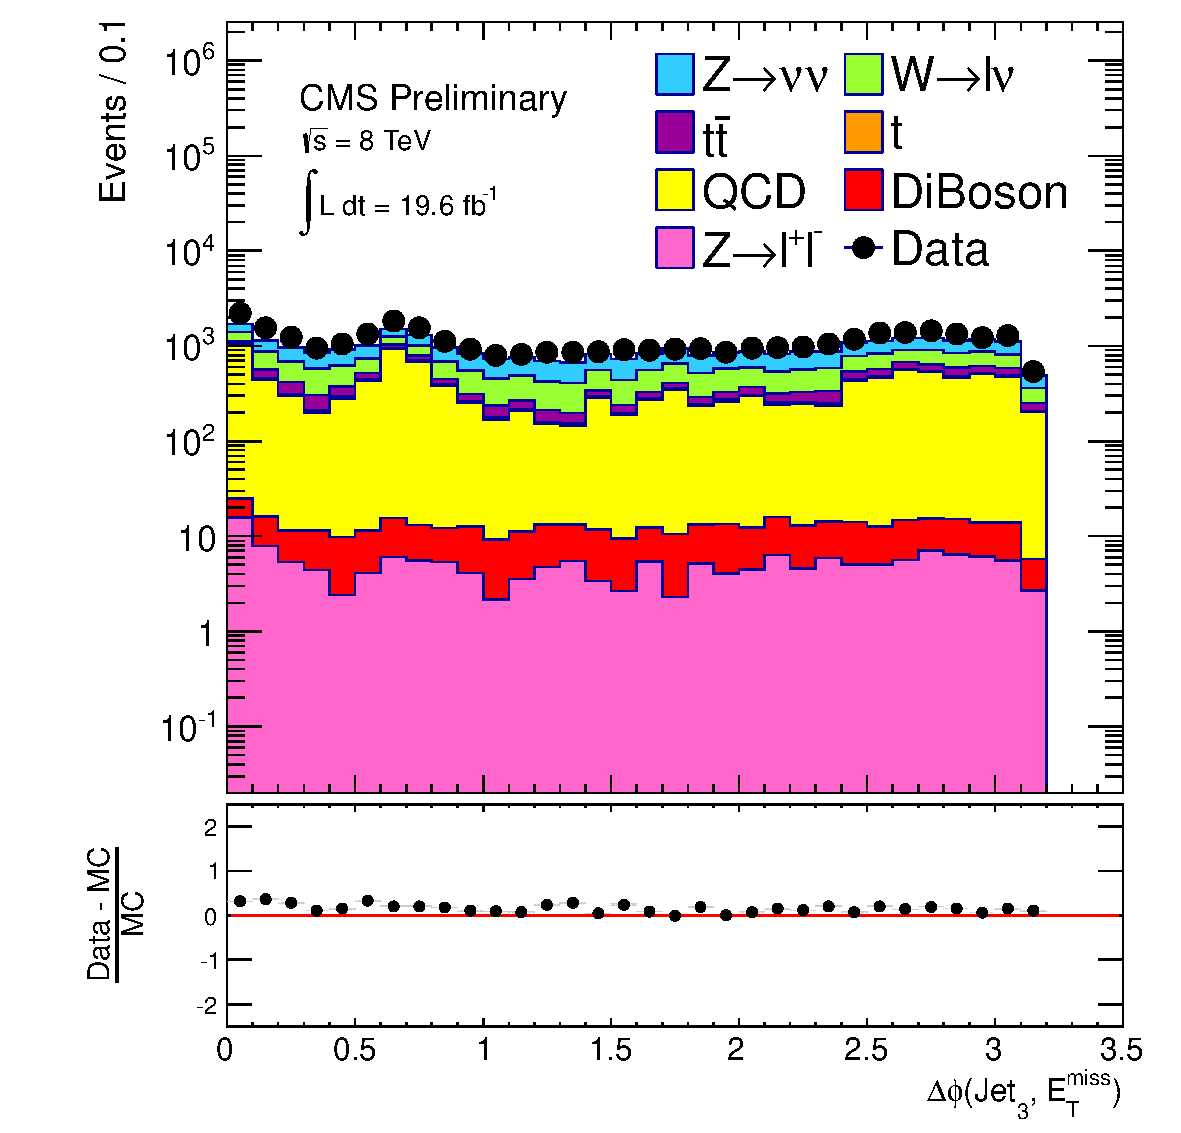
\includegraphics[scale=0.4]{Figures/sus13009/dPhi_MetLep_Jet3.pdf}
 \caption{ $\Delta \phi(\,\mathrm{\MET}, \,\mathrm{j}_3)$, shown for a jet counting threshold of 60~\GeV{} for $\pt(\,\mathrm{j}_1)>250$~\GeV.}
 \label{dphi_METj3}
 \end{center}
 \end{figure}


\subsection{\ttbar background estimation}
\label{sec:ttbar}
The contribution of \ttbar events in the search regions is predicted to be small, $\approx2\%$.
It is estimated using simulation normalized using the \ac{NNLO} cross section~\cite{ttbarxs}, 
and cross checked using a data control sample enriched in \ttbar events. 
The data control sample is derived from the same trigger as the search regions, satisfying the selection criteria of $\METmu>250~\GeV$ and $\pt(\jet_1)>110~\GeV$, along with the event cleaning criteria. 
In addition, $\Delta \phi(\jet_1, \jet_2)<2.5$, and, to select leptonic decays of \ttbar events, 
a well-identified electron is required, and a loose muon of opposite sign. 
The invariant mass of the electron-muon system must lie above 60~\GeV, removing much of the contribution of \zellellbr{}\,+\,jets events in the control sample. 

The distributions of the invariant mass and \pt{} of the electron-muon system are shown in Figure~\ref{ttbar}.
The event yields from data and simulation are shown in 
Table~\ref{ttbartable}, before and after the invariant mass cut.  
Data and simulation are seen to agree well with one another.
The scale factor $R^{\ttbar}$ is extracted using an analogous method as for $R^{\rm QCD}$, and has a value of 0.97$\pm$0.3, where the uncertainty is dominated by the systematic uncertainty in the non-\ttbar processes in the control sample, 
which are taken as 50\% of each.
We therefore find that the \ac{NNLO} cross section used to normalize the \ttbar simulation describes the data well, and apply a data/MC scaling factor of 1.0.

Although probably over-conservative, the uncertainty on the \ttbar background is taken to be 50\% to be consistent with the other background estimations taken from simulation. 
% it covers uncertainties in the \ac{PDF}s, hadronization modelling,  

\newsavebox{\cutflowBoxj}
\begin{table}[htdp!]
\caption{Event yields from MC and data for $t\bar{t}$ background}
\begin{center}
\begin{lrbox}{\cutflowBoxj}
\begin{tabular}{c|cccccccc}
\hline
Requirement &   $1 \e, 1 \mu$  &   $m_{T}(\e \mu) > 60~\GeV$ \\ \hline
\ttbar               & 421 & 375 \\
Single top           & 61  & 55  \\
\zellellbr{}\,+\,jets  & 51  &  7  \\
Diboson              & 34  & 27  \\
\wpj{}                 & 2   & 0.5 \\
QCD                  & 0   & 0    \\ \hline
Total background     & 568 & 464  \\
Data & 554 & 452 \\ \hline
Data/MC   & 0.98 & 0.97 \\ \hline
\end{tabular}
  \end{lrbox}
  \scalebox{0.87}{\usebox{\cutflowBoxj}} 
\label{ttbartable}
\end{center}
\end{table}


\begin{figure}[htbp!]
\begin{center}
  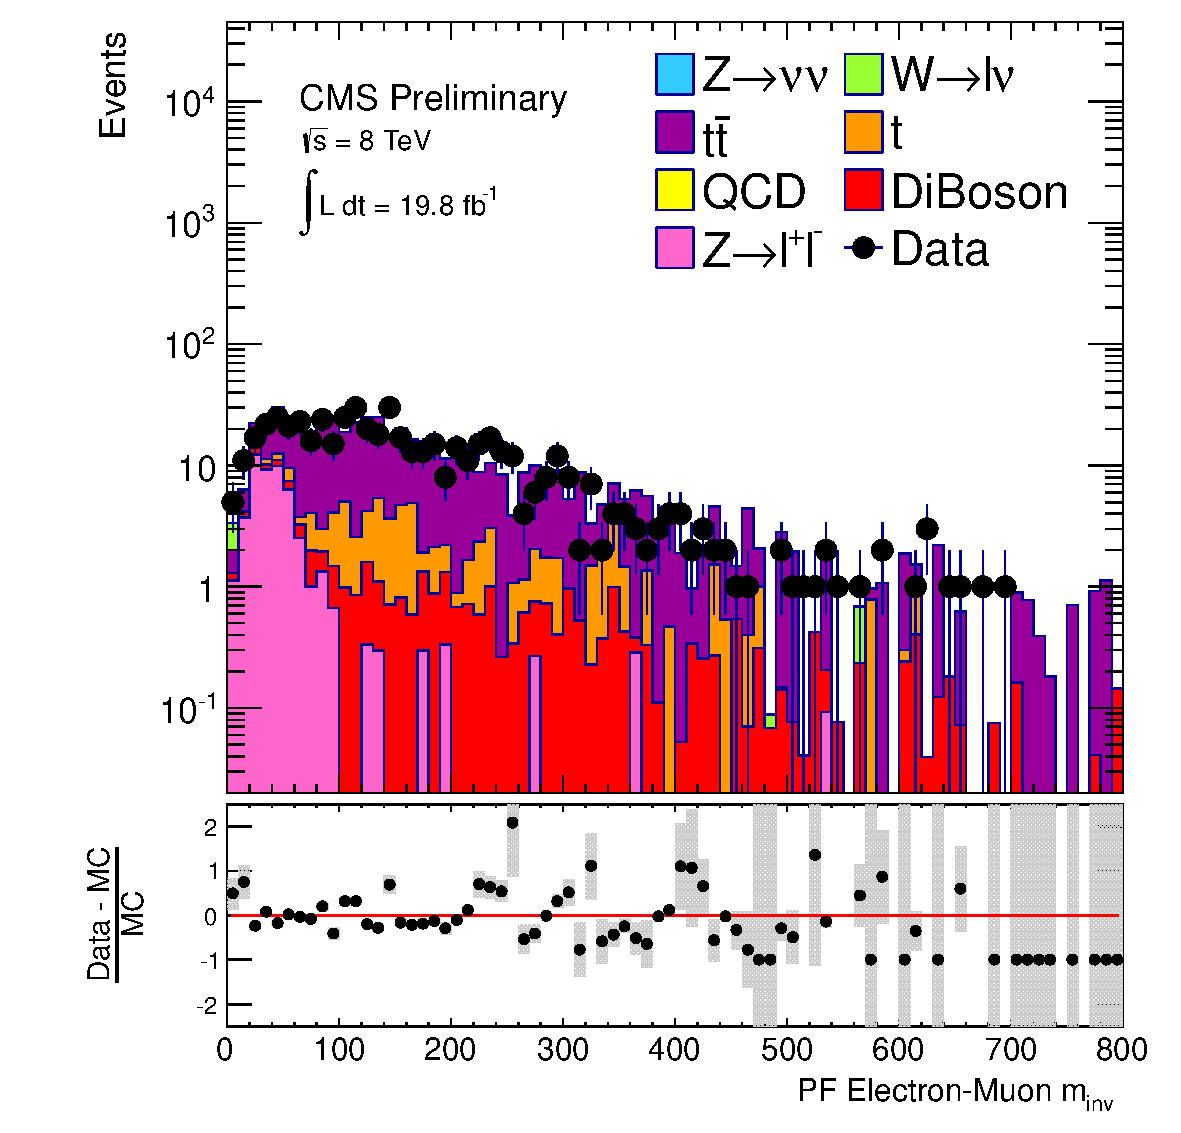
\includegraphics[scale=0.35]{Figures/sus13009/PFElecMuonMass.pdf} 
    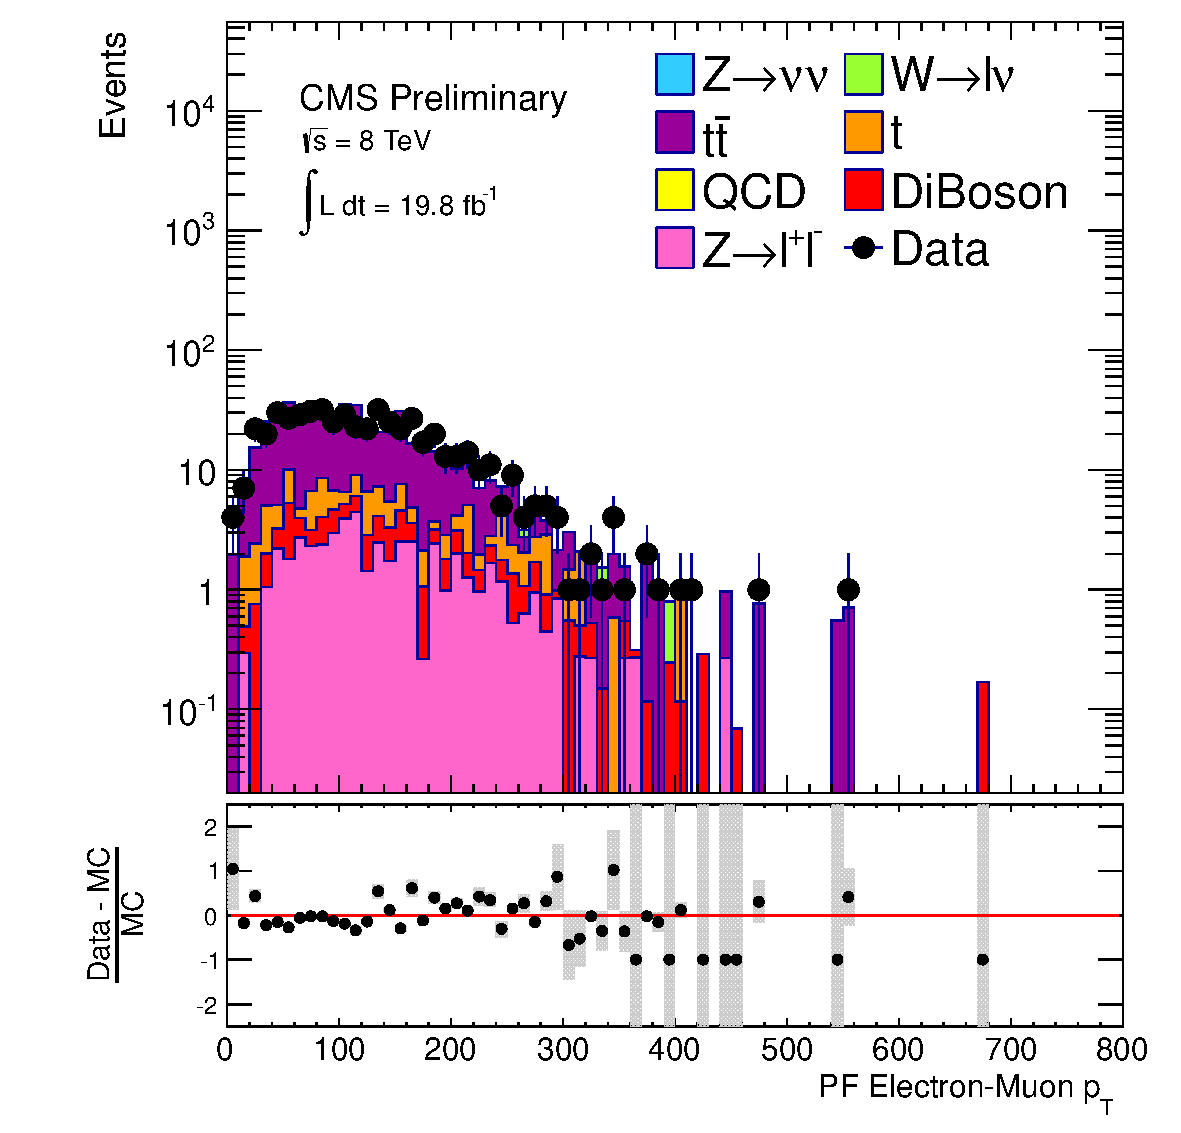
\includegraphics[scale=0.35]{Figures/sus13009/PFElecMuonPt.pdf}
\caption{Invariant mass distribution (left) and \pt{} distribution (right) of the $\e\mu$ pair in the \ttbar-enriched control sample.}
\label{ttbar}
\end{center}
\end{figure}



\subsection{Diboson background estimation}
%The remaining backgrounds to the monojet sample from \ttbar, QCD, single top and Z\,+\,jets events are found to be at the 5\% level. These are taken from MC and assigned a 50\% systematic uncertainty.
The diboson (WW, WZ and ZZ) backgrounds are estimated using simulation, where the NLO cross sections~\cite{MCFM:diboson} are used to normalize event yields to the integrated luminosity of the search regions. 
The diboson backgrounds where one of the bosons is a photon, V$\gamma$: $\W\gamma$, $\znunubr \gamma$ and $\zellellbr \gamma$, are treated inclusively: they are absorbed into the data driven estimates of \wpj{} and \znunubr{}\,+\,jets, 
and into the MC estimate of \zellellbr{}\,+\,jets respectively. 

Table~\ref{tab:incl_excl} shows the difference between treating the $\rm{V}\gamma$ backgrounds inclusively as opposed to exclusively --- taking their yields in the search regions individually from simulation.
The difference in evaluating the \znunubr{}\,+\,jets event yield with and without the inclusion of $\znunubr \gamma${}\,+\,jets is calculated, in order to give a data-driven estimation of the $\znunubr \gamma${}\,+\,jets background.
This method is compared to the yield from using simulation directly.
A similar method is used to compare the yield of $\W \gamma${}\,+\,jets in data and simulation.
Both agree within the 50\% uncertainty assigned to all numbers taken from simulation. 

\newsavebox{\cutflowBoxi}
\begin{table*}[ht]
        \begin{center}
     \caption{Inclusive and exclusive methods of treating $\znunubr \gamma$ and $\W\gamma$ backgrounds. Data driven estimates are calculated to be the difference between the methods, and are compared to event yields from simulation.}

 \label{tab:incl_excl}
 \begin{lrbox}{\cutflowBoxi}                      
 \begin{tabular}{l|ccccccc}
 \hline
 $\pt(\,\mathrm{j}_1)$ (\GeV)  & $>250$ &$>$300 & $>350$ & $>400$& $>450$ & $>500$ & $>550$ \\ \hline
\multicolumn{8}{c}{Z($\nu\nu$)\gamma \,+\,jets}  \\ \hline 
\znunubr\,+\,\znunubr$\gamma$\,+\,jets$^{\rm data}$
      & 21209$\pm$1115 & 10077$\pm$592  & 4597$\pm$324 & 2250$\pm$197 & 1250$\pm$137 & 663$\pm$94  & 334$\pm$65 \\
\znunubr{}\,+\,jets$^{\rm data}$
      & 20104$\pm$1328 & 9508$\pm$715 & 4339$\pm$379 & 2156$\pm$215 & 1200$\pm$145 & 634$\pm$99 & 317$\pm$68 \\ 
$\znunubr \gamma$\,+\,jets$^{\rm data}$
      & 1105  & 569   & 258  & 94   & 50   & 29   & 17 \\
$\znunubr \gamma$\,+\,jets$^{\rm MC}$
      & 1289  & 595  & 274  & 148  & 50   & 26   & 15 \\ \hline
Data / MC
      & 0.86  & 0.96  & 0.94 & 0.64 & 1.00 & 1.12 & 1.13 \\ \hline

\multicolumn{8}{c}{$\W \gamma$\,+\,jets}  \\ \hline 
\W\,+\,$\W\gamma$\,+\,jets$^{\rm data}$ & 12328$\pm$707   & 5939$\pm$366  & 2690$\pm$180 & 1246$\pm$92 & 627$\pm$52 & 301$\pm$29 & 150$\pm$18 \\
\wpj$^{\rm data}$   & 11831$\pm$747 & 5677$\pm$388 & 2562$\pm$188 & 1186$\pm$98 & 592$\pm$53 & 288$\pm$31 & 139$\pm$19 \\
$\W\gamma$\,+\,jets$^{\rm data}$     & 497  & 262  & 128  & 60   & 35   & 13   & 12   \\          
$\W\gamma$\,+\,jets$^{\rm MC}$          & 503  & 271  & 134  & 62   & 38   & 13   & 11   \\ \hline   
Data / MC       & 0.99 & 0.97 & 0.96 & 0.97 & 0.92 & 1.00 & 1.09 \\ \hline 
\end{tabular} 
  \end{lrbox}
  \scalebox{0.75}{\usebox{\cutflowBoxi}} 
\end{center}
\end{table*}

A fluctuation in the ratio of data to MC simulation is observed in the estimation of $\znunubr \gamma$\,+\,jets, for $\pt(j1) > 400$ GeV.
This is due to a statistical upward fluctuation in the $\znunubr \gamma$ simulation around $\pt=400$~\GeV.
Fitting the data/MC numbers in each $\pt(\,\mathrm{j}_1)$ search region with a straight line, 
such a fluctuation is not observed and the data/MC ratio at $\pt(j1) > 400$ GeV becomes 0.9.



By absorbing $\W\gamma$ and $\znunubr \gamma$ events into the dominant data driven backgrounds 
we not only get a better estimation of these backgrounds as we do not rely on the simulation 
(which does not necessary represent the data accurately in this area of phase space), 
we also reduce the uncertainty on the estimations, 
and in doing so reduce the total uncertainties of the analysis.
This is because the yields (in simulation) of $\W\gamma$ and $\znunubr \gamma$ no longer contribute to $N^{\rm bkg}_{\mu\mu}$ and $N^{\rm bkg}_{\mu}$, so the 50\% uncertainties on the yields are also no longer included in the uncertainty calculation on these numbers. 
Instead, they are accounted for within the $N^{\rm obs}_{\mu\mu}$ and $N^{\rm obs}_{\mu}$ yields with uncertainties calculated as discussed above.


\subsection{Single top quark and Drell--Yan background estimations}

Backgrounds due to single top quark events are predicted to be very small, of order 0.5\%.
Yields are taken directly from simulation and normalized to the approximate \ac{NNLO} cross sections~\cite{ttbarxs}. 
The contribution of Drell--Yan $\zellellbr$\,+\,jets processes in the search regions are predicted to be of a similar size, due to the lepton vetoes - contributing $\approx0.5\%$.
It is combined with the background due to $\zellellbr \gamma$ processes, which is negligible and only included for completeness,
and evaluated using simulation.
An uncertainty of 50\% is assigned to these predictions.


\section{Summary}
Selection has been presented to reduce \ac{SM} background contribution and maximise possible signal acceptance. 
The contribution of SM \ttbar and multijet events in the search regions is reduced using topological selections. The dominant backgrounds after the complete event selection are from \znunubr{}\,+\,jets and \wpj{} events. These are estimated using muon data control samples enriched in \zmumubr and \wmunubr events. Remaining background from \ttbar and multijet processes are estimated using simulation normalized in data control samples, and small contributions of diboson, \zellellbr, and single top quark events are taken from simulation.


